\documentclass[aspectratio=169]{beamer}
%\usepackage{pgfpages}
%\pgfpagesuselayout{4 on 1}[a4paper,border shrink=5mm]
\usetheme[block=fill,progressbar=frametitle,numbering=none]{metropolis}
\usepackage{animate}
% Paquetes de la ams
\usepackage{amsmath,amsthm,amssymb,amsfonts}
% Codificacion UTF-8
\usepackage[utf8]{inputenc}
% Tablas e imagenes en espaniol
\usepackage[spanish,es-tabla]{babel}
% Mejores graficos
\usepackage{graphicx}
% tablas mas lindas
\usepackage{booktabs}
% Links a urls
\usepackage{url}
% Linkear referencias en pdfs
\usepackage{hyperref}
% Texto mas lindo para los pie de figura
\usepackage[margin=10pt,font=small,labelfont=bf, labelsep=endash]{caption}

% Citas
\usepackage[backend=biber,style=ieee]{biblatex}
\addbibresource{biblio.bib}

% Codigo
\usepackage{listings}

% Dir tree
\usepackage{dirtree}

% Pagina en blanco cuando ha
\usepackage{emptypage}

\definecolor{A11}{HTML}{B2DF8A}
\definecolor{A12}{HTML}{33A02C}
\definecolor{A23}{HTML}{FDBF6F}
\definecolor{A24}{HTML}{FF7F00}
\definecolor{B15}{HTML}{FB9A99}
\definecolor{B16}{HTML}{E31A1C}
\definecolor{B27}{HTML}{A6CEE3}
\definecolor{B28}{HTML}{1F78B4}

% Ejemplos, observaciones y teorema
\theoremstyle{definition}
\newtheorem{exa}{Ejemplo}[section]
\newtheorem*{obs}{Observación}
\newtheorem{que}{Pregunta}[section]
\newtheorem{dex}{Definicion}[section]

\usepackage{multimedia}
\usepackage{subfig}
\includeonly{clase5}
\title{Introducción a la teledetección SAR}
\subtitle{Curso Nivel 2:}

\author{Francisco Nemiña$^{*}$ \and Tomás Zajc$^{**}$}


\institute{$^{*}$ Unidad de Educación y Formación Masiva, Comisión Nacional de Actividades Espaciales\\
$^{**}$ Misión SAOCOM, Comisión Nacional de Actividades Espaciales}

\date{}
\graphicspath{{./figs/}}

\begin{document}

\maketitle

%\begin{frame}{Esquema de la presentación}
%  \setbeamertemplate{section in toc}[sections numbered]
%  \tableofcontents[hideallsubsections]
%\end{frame}

\section{Introducción al radar}
\subsection{Espectro electromagnético}
\begin{frame}{\secname : \subsecname}
  \begin{figure}
    \centering
    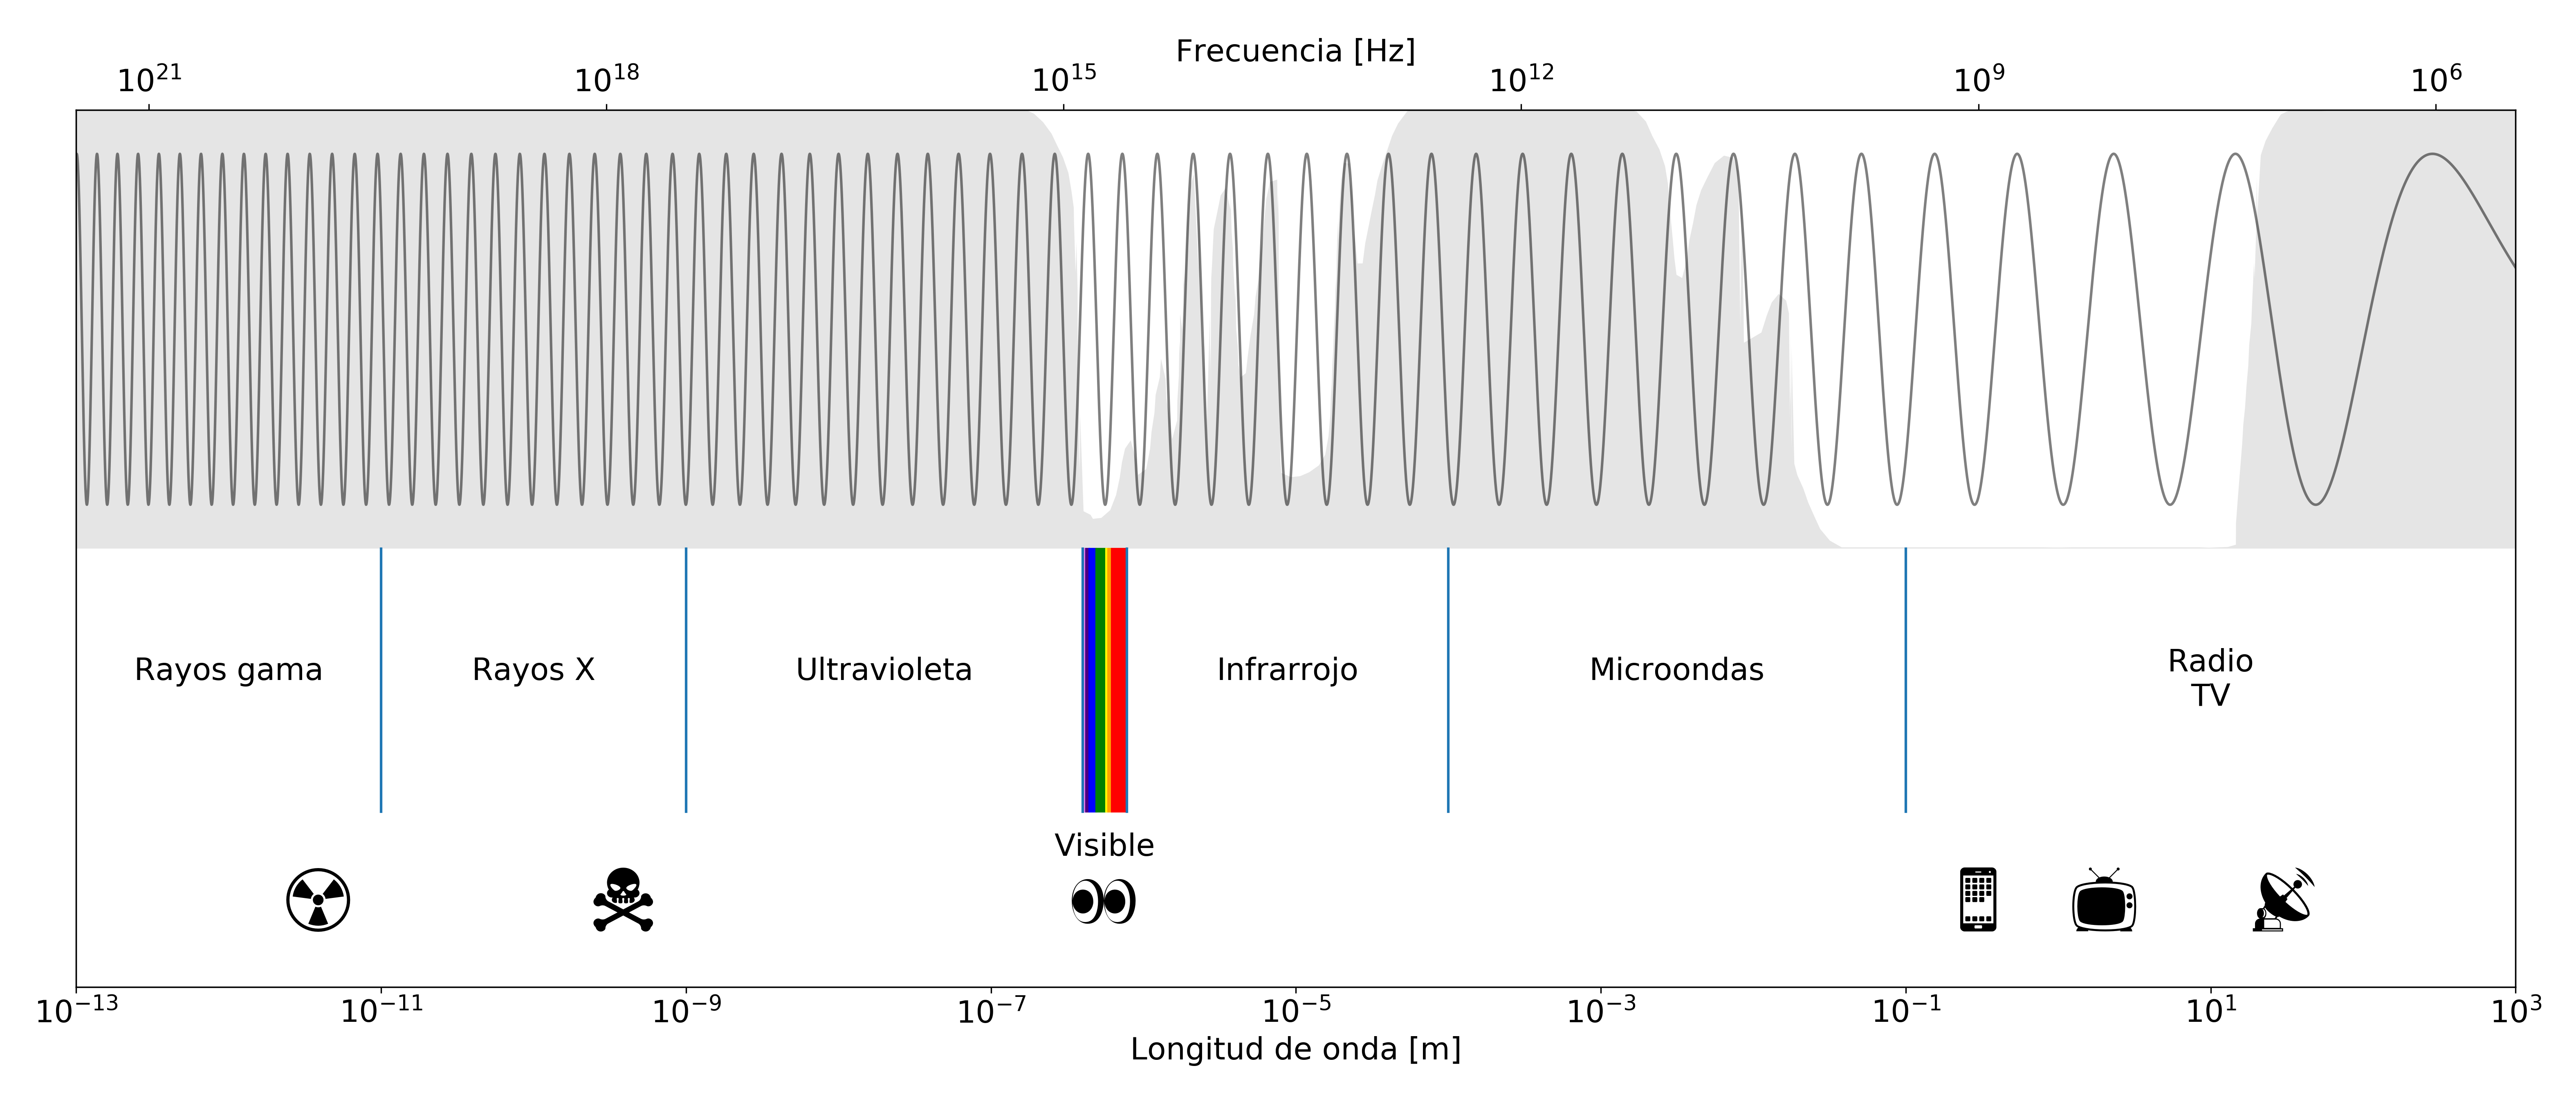
\includegraphics[width=\textwidth]{fig:espectro.png}
    \caption{Espectro electromagnético en longitud de onda (abajo) y frecuencia (arriba).}
    \label{}
  \end{figure}
\end{frame}
%--- Next Frame ---%

\subsection{¿Qué es un radar?}
\begin{frame}{\secname : \subsecname}
    \begin{figure}
      \centering
      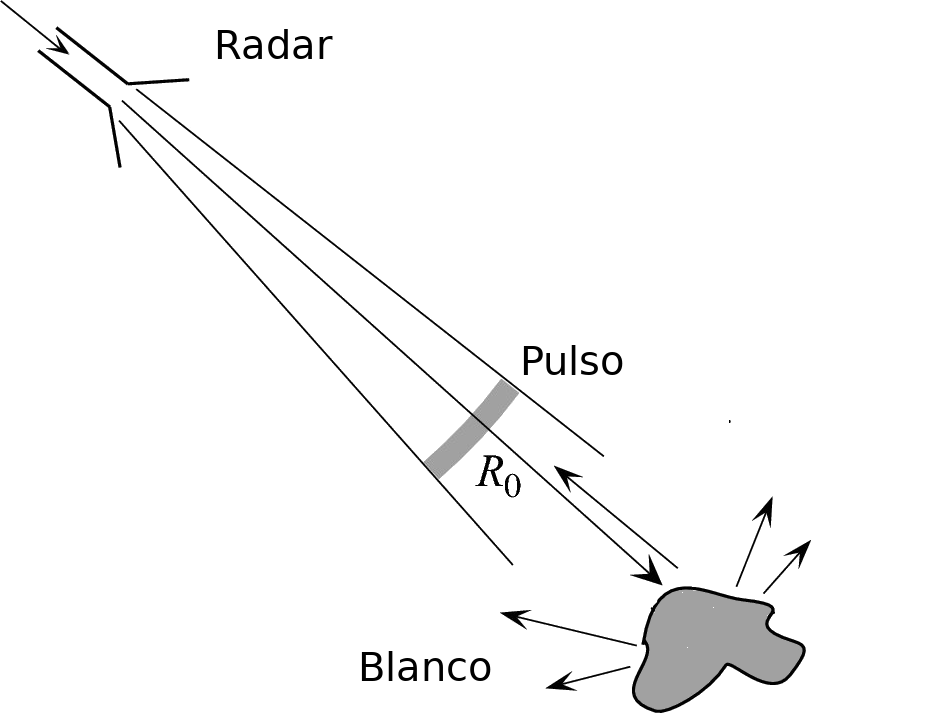
\includegraphics[scale=0.7]{fig:radar.png}
      \caption{RAdio Detection And Ranging. Funcionamiento esquemático.}
      \label{}
    \end{figure}
\end{frame}
%--- Next Frame ---%

\subsection{¿Cómo detecta un radar?}
\begin{frame}{\secname : \subsecname}
  \begin{figure}
    \centering
    \movie[width = \textwidth,loop,autostart]{\centering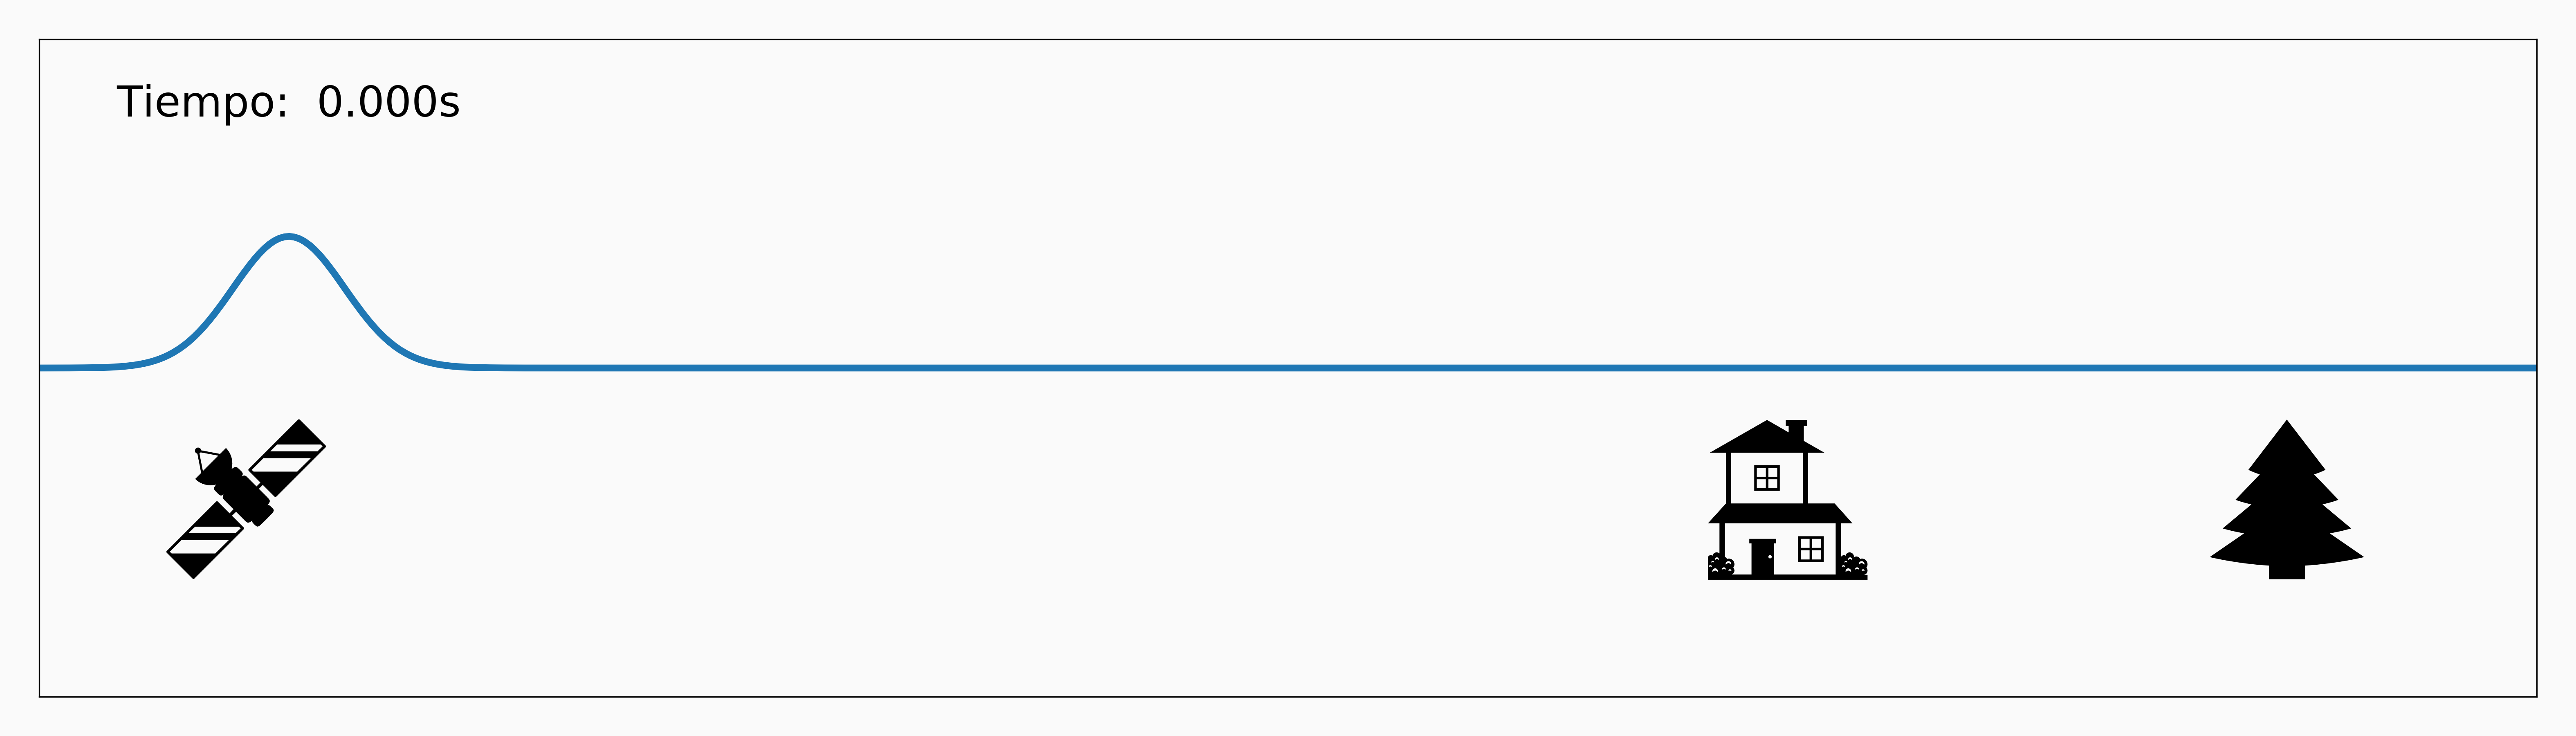
\includegraphics[width=\textwidth]{fig:funcionamiento.png}}{./figs/fig:funcionamiento.mp4}
    \caption{Ecos detectados por un radar en función del tiempo}
    \label{}
  \end{figure}
\end{frame}
%--- Next Frame ---%

\subsection{Geometría}
\begin{frame}{\secname : \subsecname}
  \begin{figure}
    \centering
    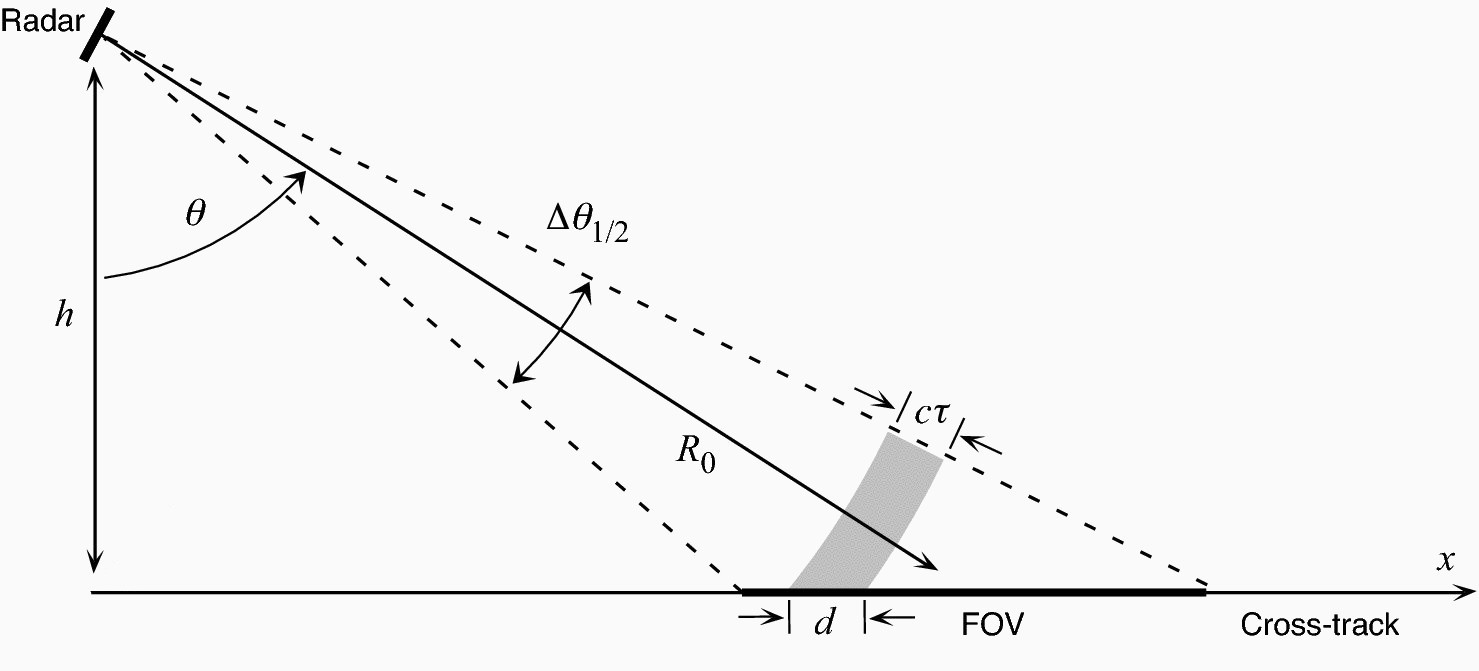
\includegraphics[scale=0.7]{01938fig10_3.jpg}
    \caption{Geometría de observación de un radar en dos dimensiones viso en un corte transversal.}
    \label{}
  \end{figure}
\end{frame}
%--- Next Frame ---%

\subsection{Generación de una imagen}
\begin{frame}{\secname : \subsecname}
  \begin{figure}
    \centering
    \movie[width = 0.95\textwidth,loop,autostart]{\centering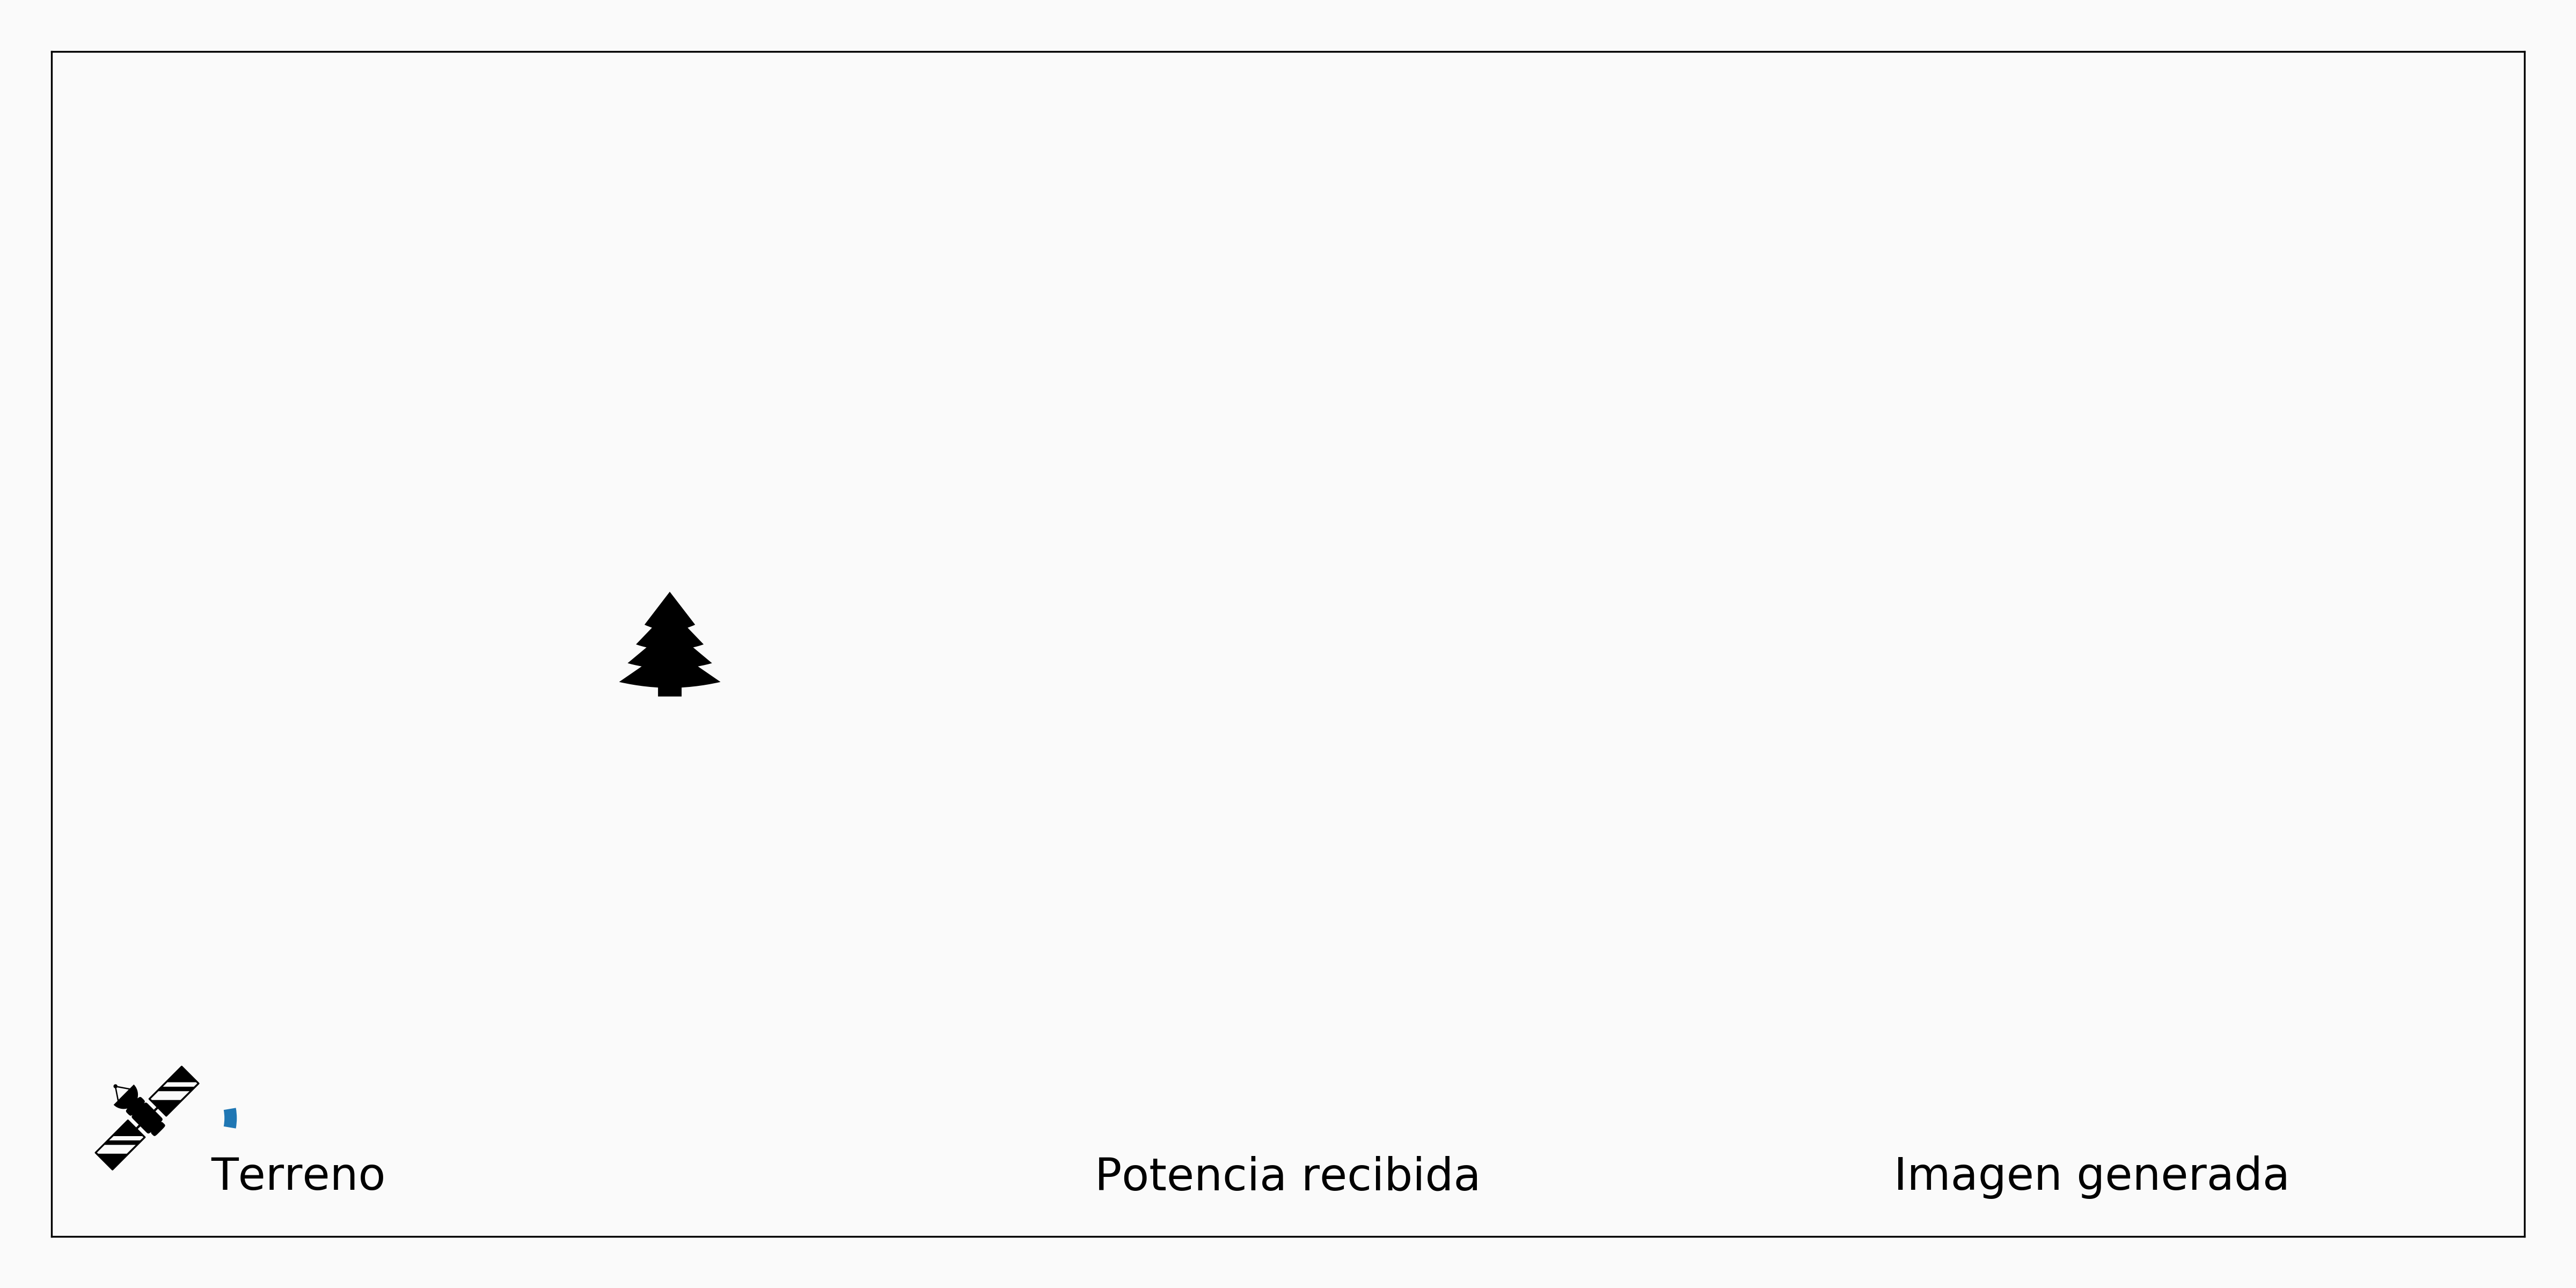
\includegraphics[width=0.95\textwidth]{fig:imagen.png}}{./figs/fig:imagen.mp4}
    \caption{Generación de una imagen radar a partir de datos en el terreno.}
    \label{}
  \end{figure}
\end{frame}
%--- Next Frame ---%


\begin{frame}{\secname : \subsecname}
  \begin{figure}
    \centering
    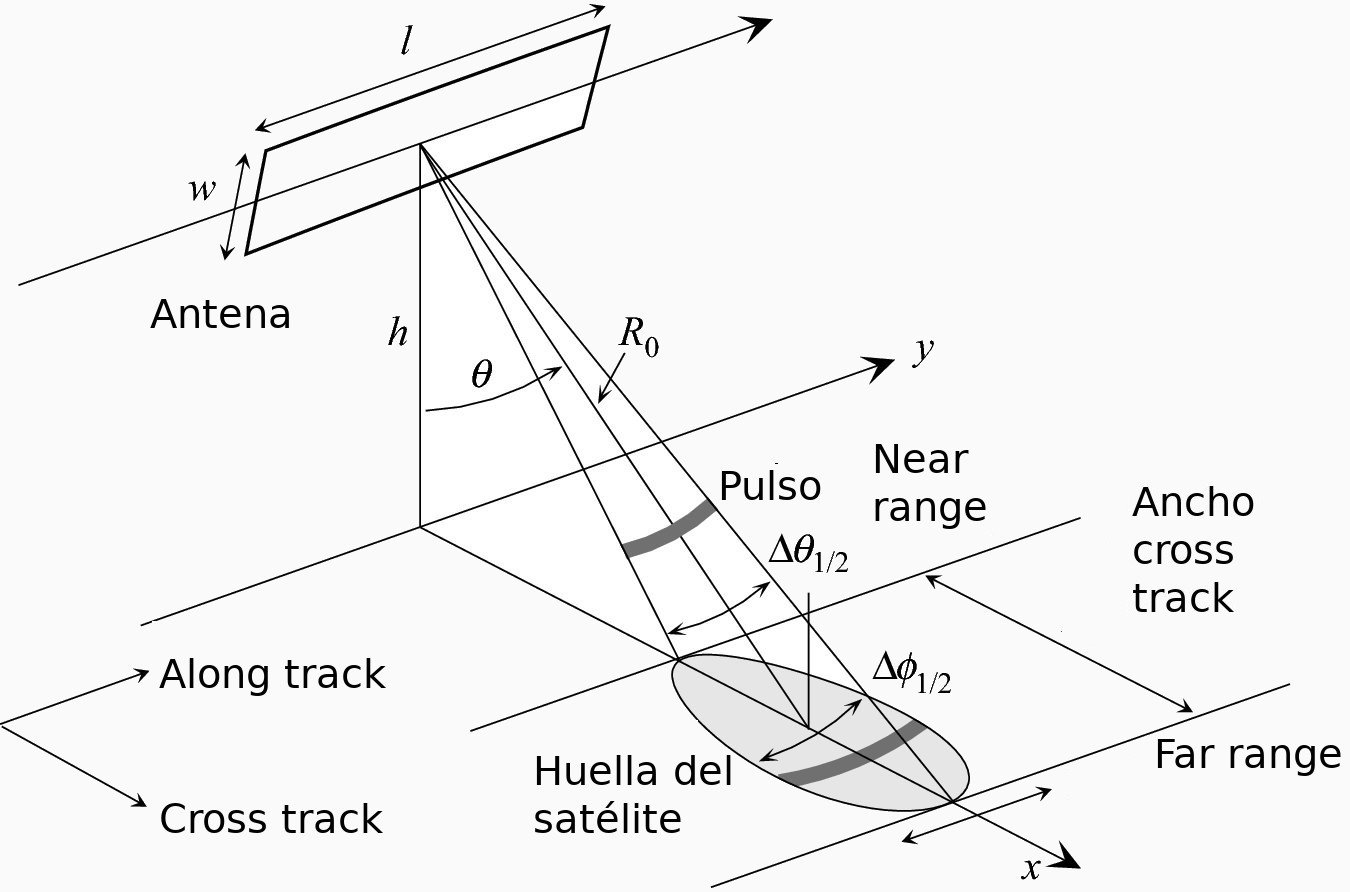
\includegraphics[scale=0.7]{01938fig13_1.jpg}
    \caption{Geometría de observación de un radar completa en la direcciones perpendiculares y paralelas al movimiento (accross track y along track)}
    \label{}
  \end{figure}
\end{frame}
%--- Next Frame ---%

\subsection{Comparación con el óptico}
\begin{frame}{\secname : \subsecname}
\begin{columns}
  \begin{column}{0.5\textwidth}
   \begin{block}{Óptico}
     \begin{itemize}
       \item Rango de trabajo en los micrometros ($0.3\mu$ m a $2.5\mu m$).
       \item Detecta luz solar reflejada por la tierra.
       \item Bloqueado por las nubes.
       \item Detecta luz incoherente.
       \item Depende de una fuente de iluminación externa.
     \end{itemize}
   \end{block}
  \end{column}
  \begin{column}{0.5\textwidth}  %%<--- here
    \begin{block}{Radar}
      \begin{itemize}
        \item Rango de trabajo en los microondas ($1cm$ m a $100cm$).
        \item Emite una señal y mide la intesidad del eco.
        \item Independiente de las condiciones atmosféricas.
        \item Emite y detecta una onda coherente.
        \item Cuenta con su propia fuente de iluminación.
      \end{itemize}
    \end{block}
  \end{column}
  \end{columns}
\end{frame}
%--- Next Frame ---%

\subsection{Modos de adquisición}
\begin{frame}{\secname : \subsecname}
  \begin{figure}
    \centering
    \movie[width = 0.5\textwidth,loop,autostart]{\centering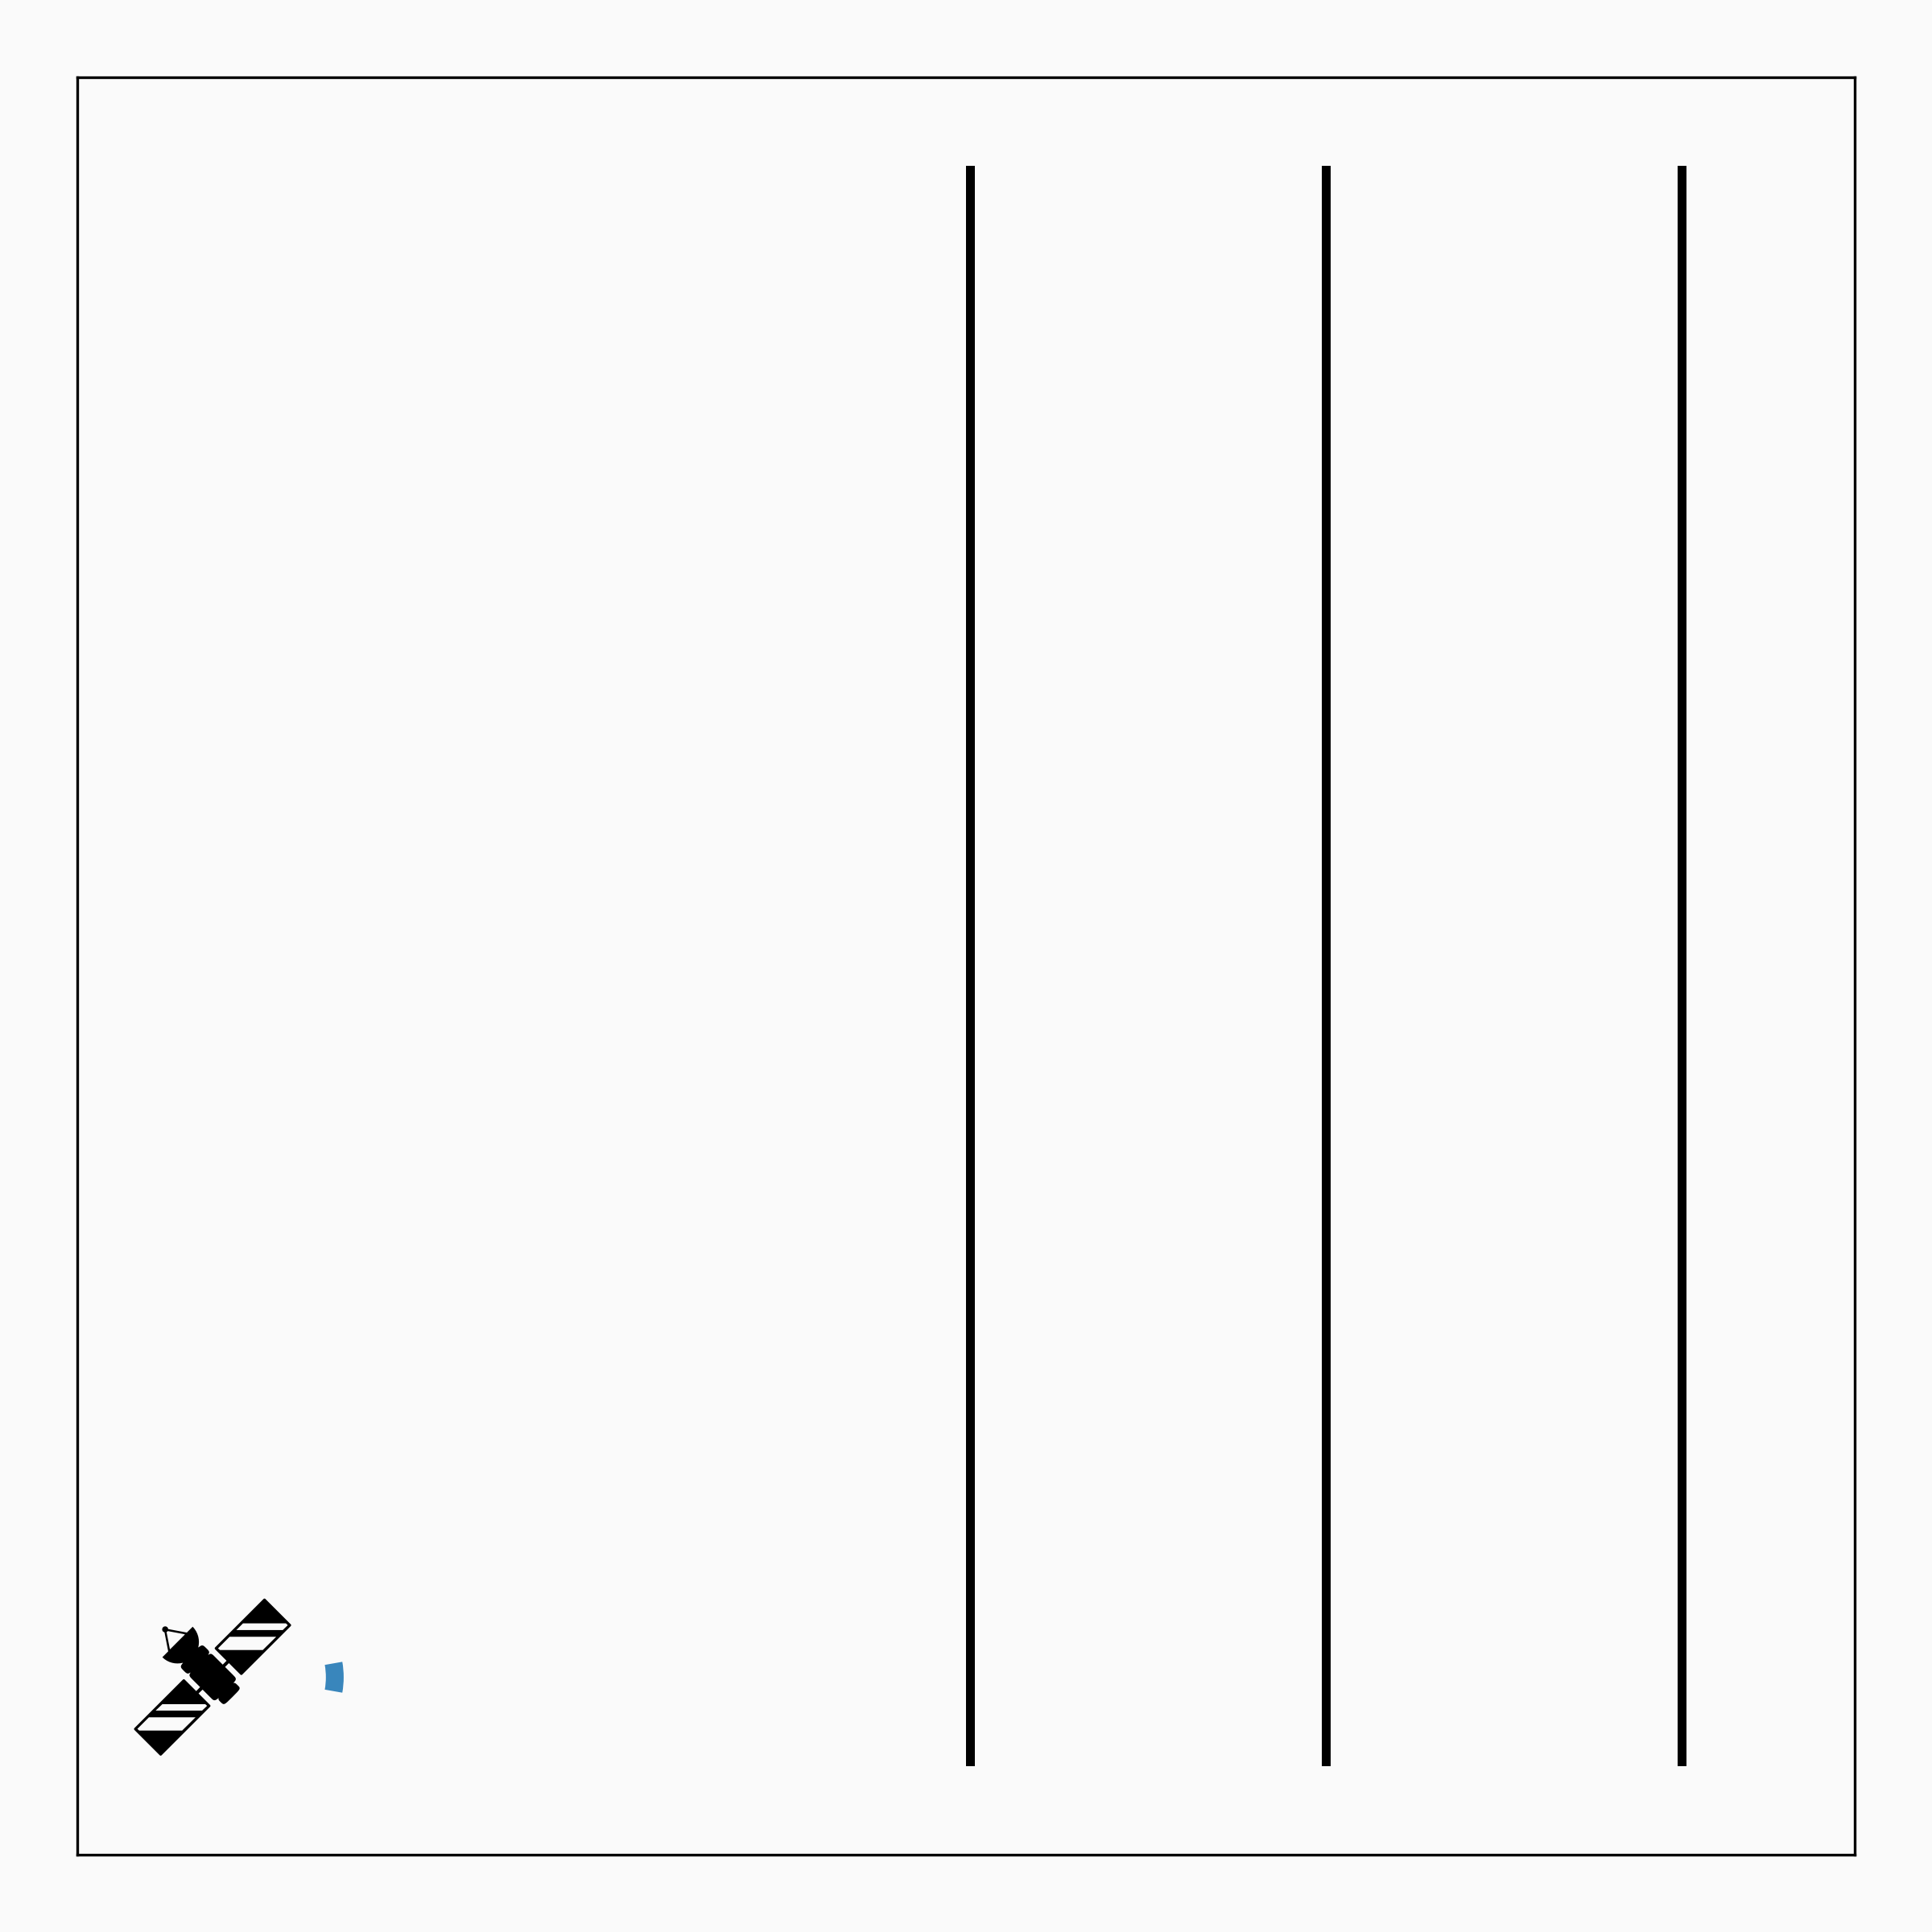
\includegraphics[width=0.45\textwidth]{fig:strip.png}}{./figs/fig:strip.mp4}
    \caption{Modo de adquisición STRIPMAP.}
    \label{}
  \end{figure}
\end{frame}
%--- Next Frame ---%

\begin{frame}{\secname : \subsecname}
    \begin{block}{Propiedades STRIPMAP}
      \begin{itemize}
        \item El RADAR toma datos de un solo Swadth
        \item Es el método de adquisición por defecto de la mayoría de los satélites.
        \item Resolución intermedia.
      \end{itemize}
    \end{block}
\end{frame}
%--- Next Frame ---%
\begin{frame}{\secname : \subsecname}
  \begin{figure}
    \centering
    \movie[width = 0.5\textwidth,loop,autostart]{\centering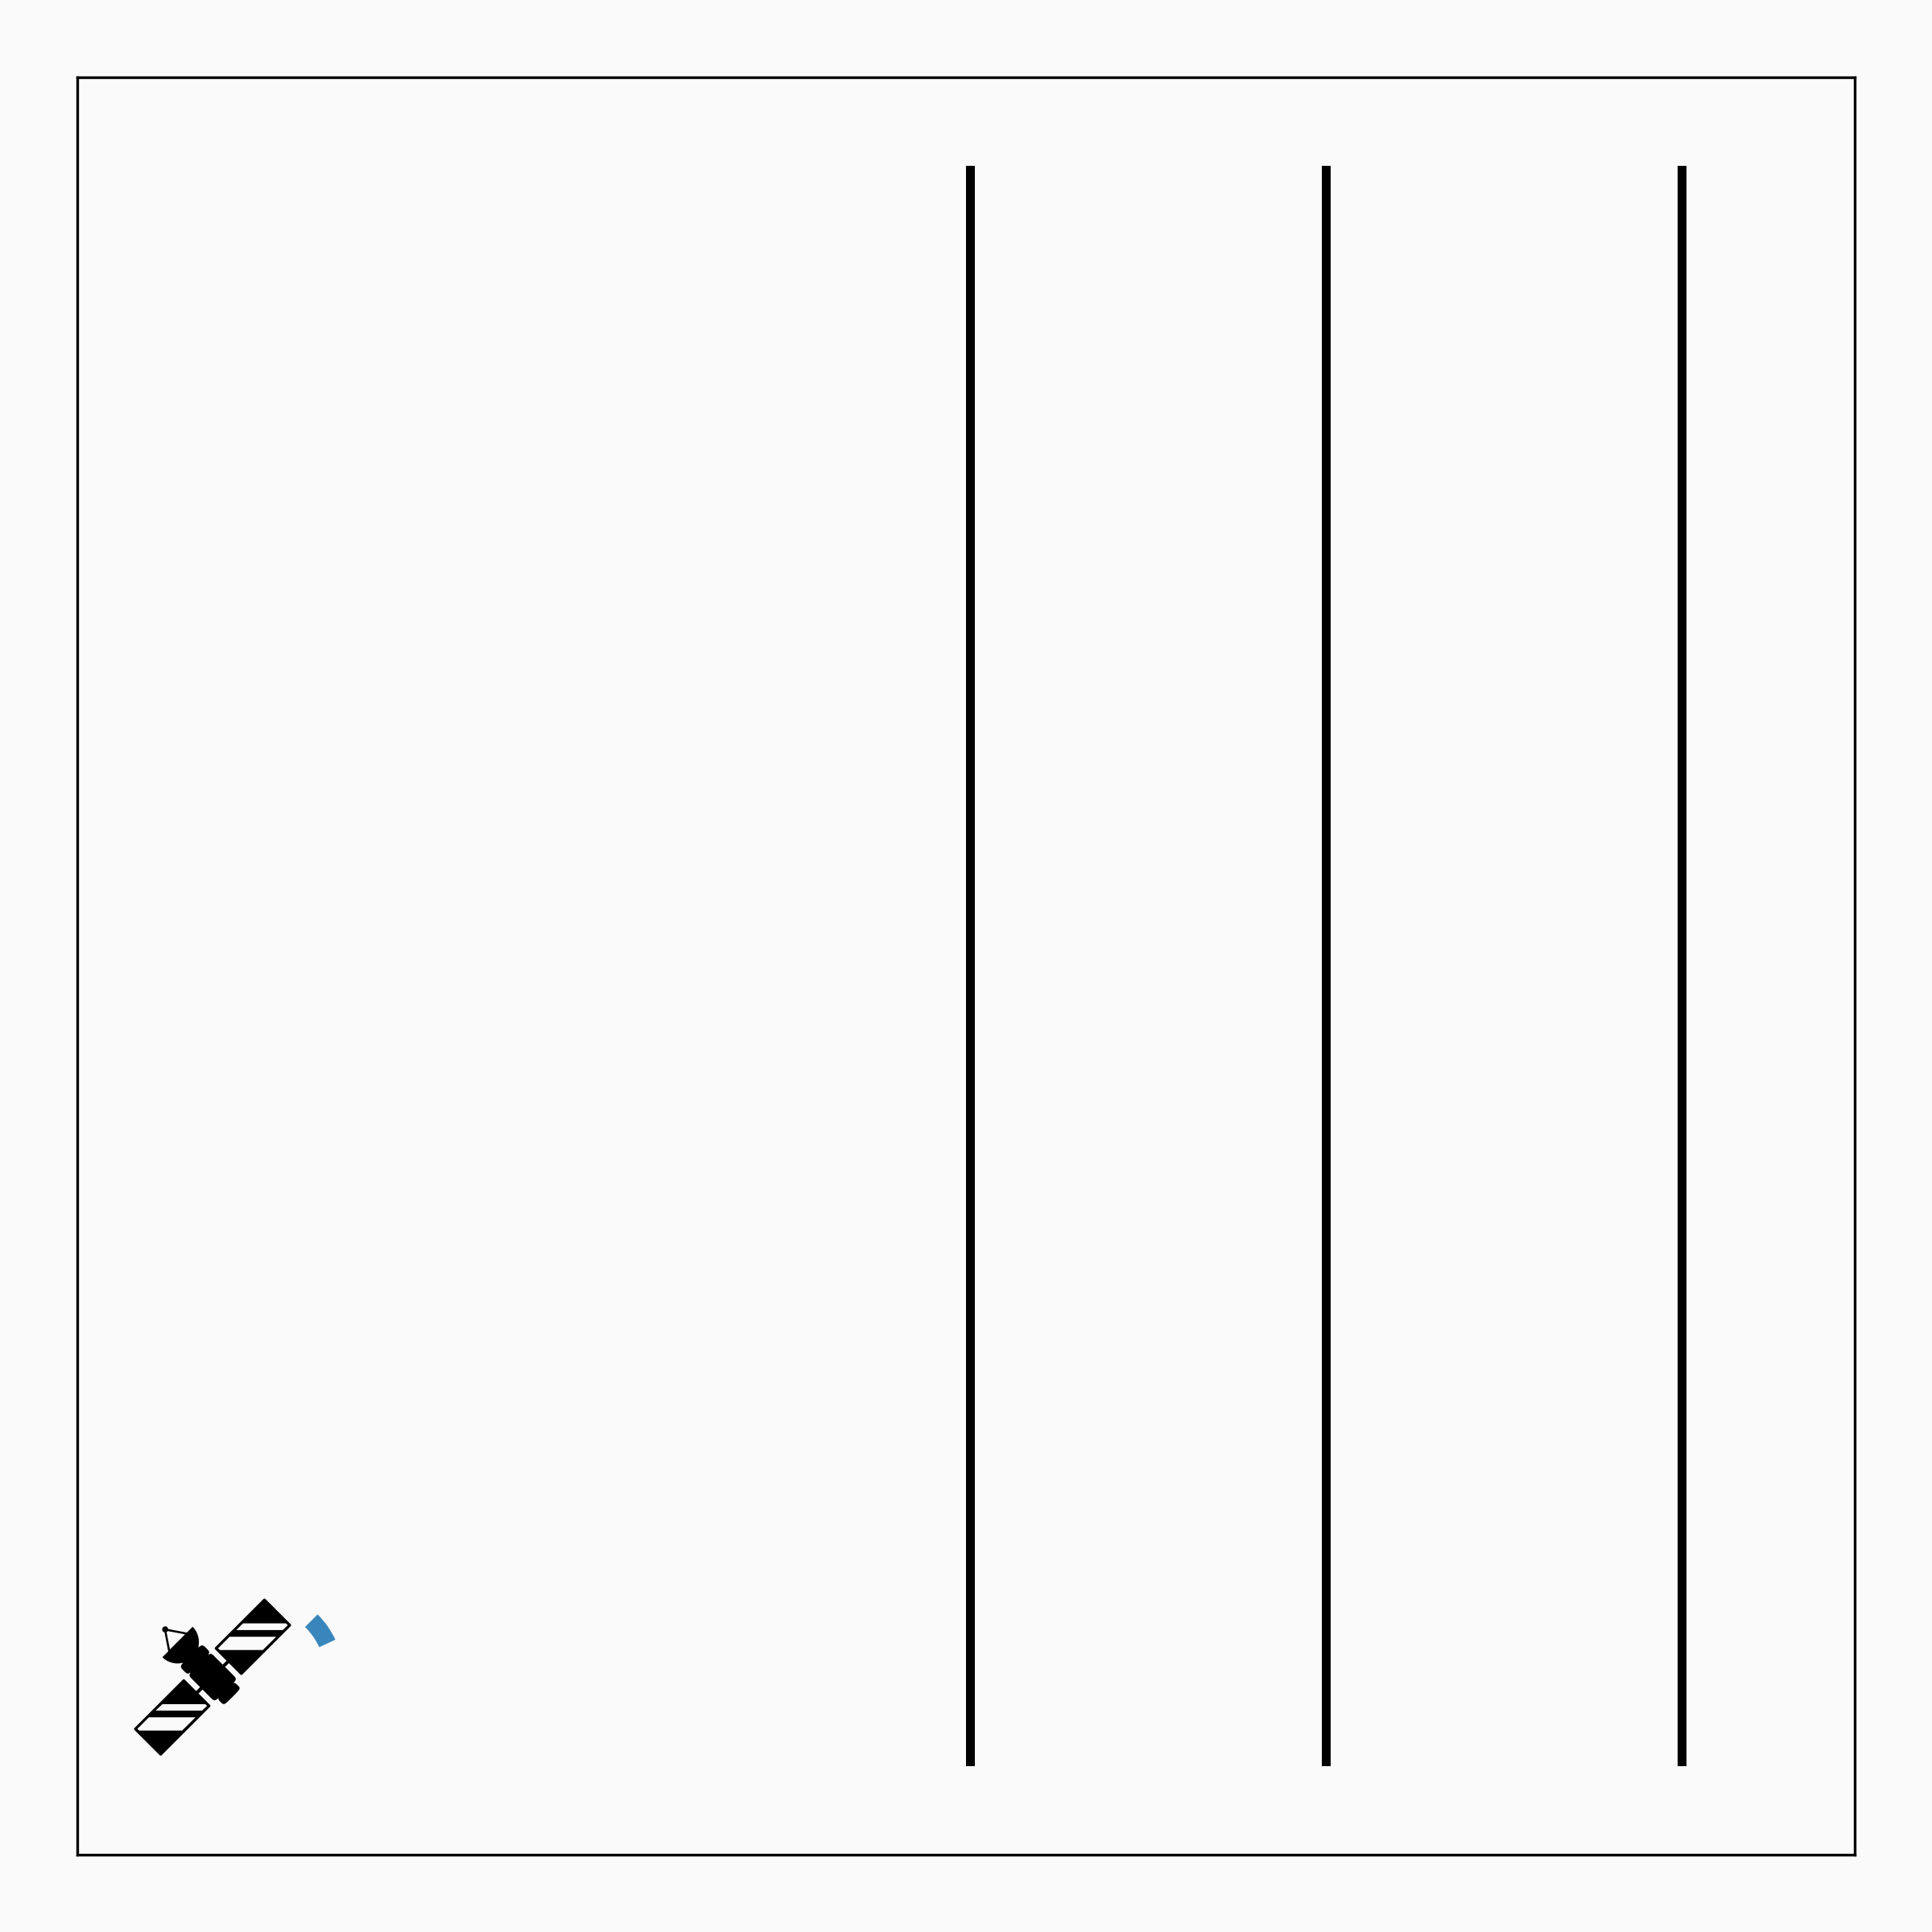
\includegraphics[width=0.45\textwidth]{fig:spot.png}}{./figs/fig:spot.mp4}
    \caption{Modo de adquisición SPOTLIGHT.}
    \label{}
  \end{figure}
\end{frame}
%--- Next Frame ---%

\begin{frame}{\secname : \subsecname}
    \begin{block}{Propiedades SPOTLIGHT}
      \begin{itemize}
        \item El RADAR enfoca la toma de datos en una región específica.
        \item Alta resolución espacial en la tema de datos.
        \item Tiene menor cobertura espacial y necesita reorientar la antena para realizar la toma de datos.
      \end{itemize}
    \end{block}
\end{frame}
%--- Next Frame ---%

\begin{frame}{\secname : \subsecname}
  \begin{figure}
    \centering
    \movie[width = 0.5\textwidth,loop,autostart]{\centering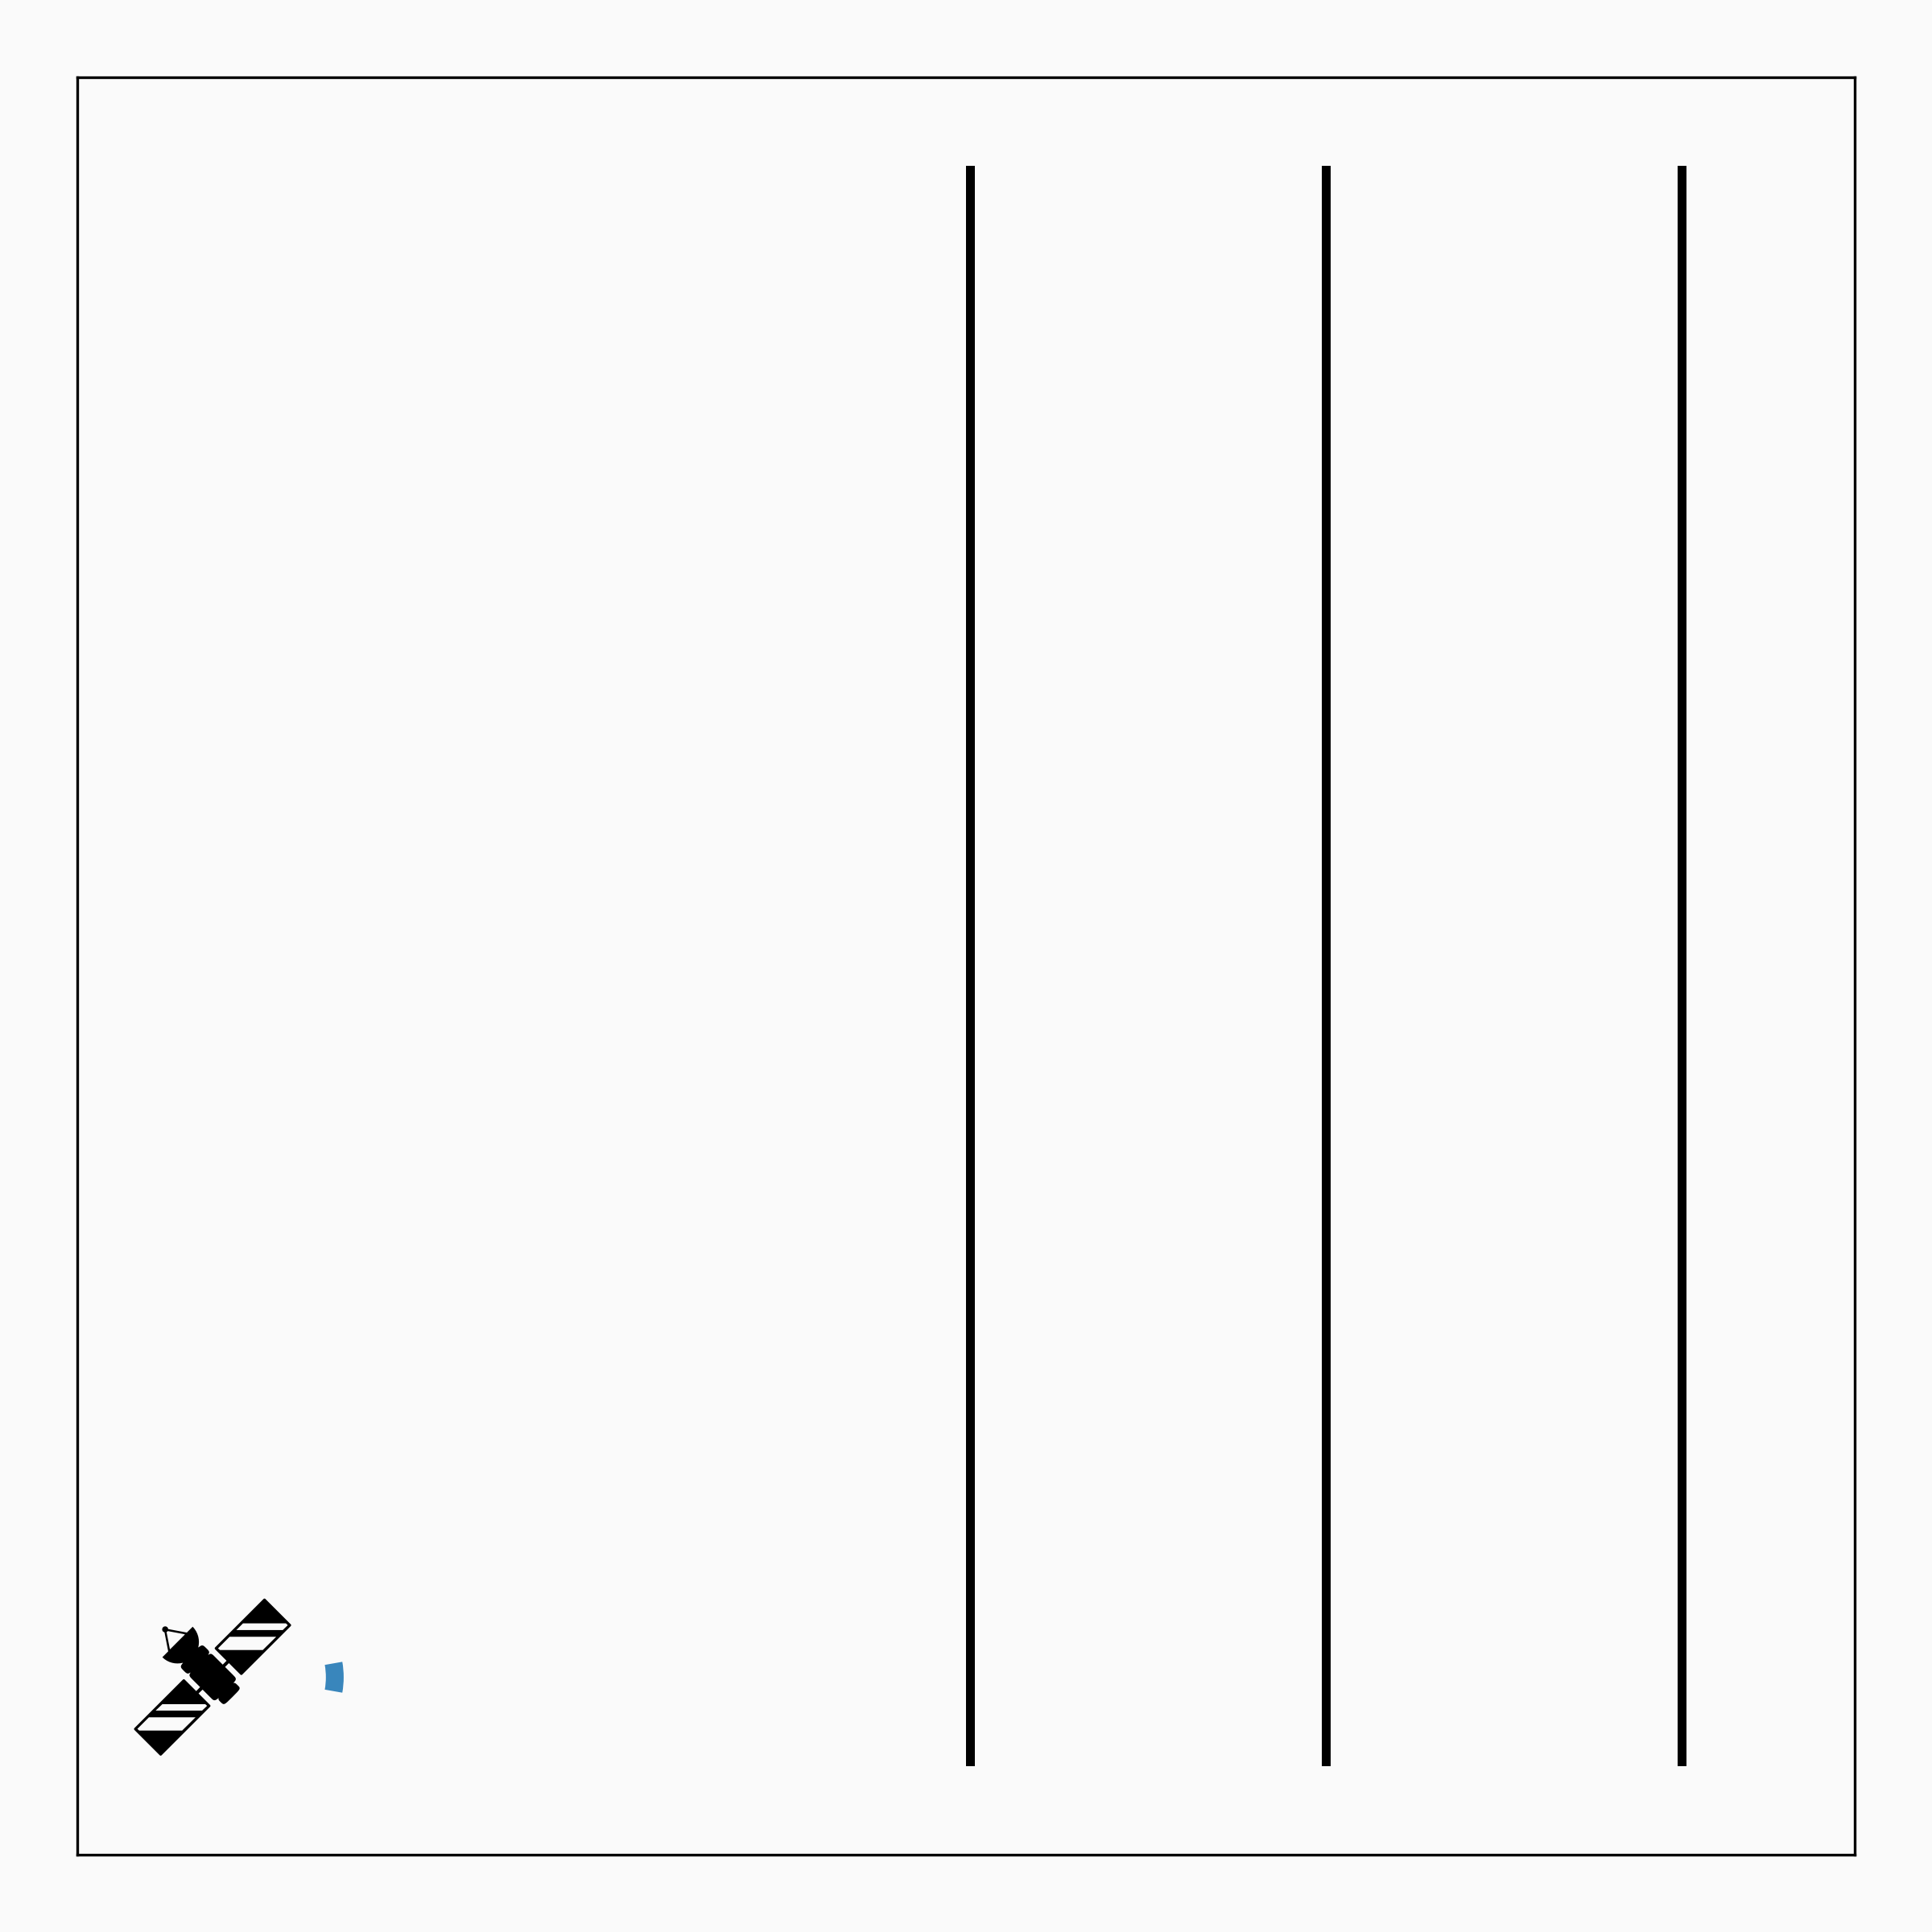
\includegraphics[width=0.45\textwidth]{fig:scan.png}}{./figs/fig:scan.mp4}
    \caption{Modo de adquisición SCANSAR.}
    \label{}
  \end{figure}
\end{frame}
%--- Next Frame ---%

\begin{frame}{\secname : \subsecname}
    \begin{block}{Propiedades SCANSAR}
      \begin{itemize}
        \item El RADAR Va distribuyendo pulsos de a bursts entre varios swaths.
        \item Gran swath.
        \item Baja resolución.
        \item Mala relación señal ruido en algunas partes y buena en otras.
        \item Mala distribución de potencia generando scalloping.
        \item Hace falta reapuntar la antena en elevación entre burst.
      \end{itemize}
    \end{block}
\end{frame}
%--- Next Frame ---%

\begin{frame}{\secname : \subsecname}
  \begin{figure}
    \centering
    \movie[width = 0.5\textwidth,loop,autostart]{\centering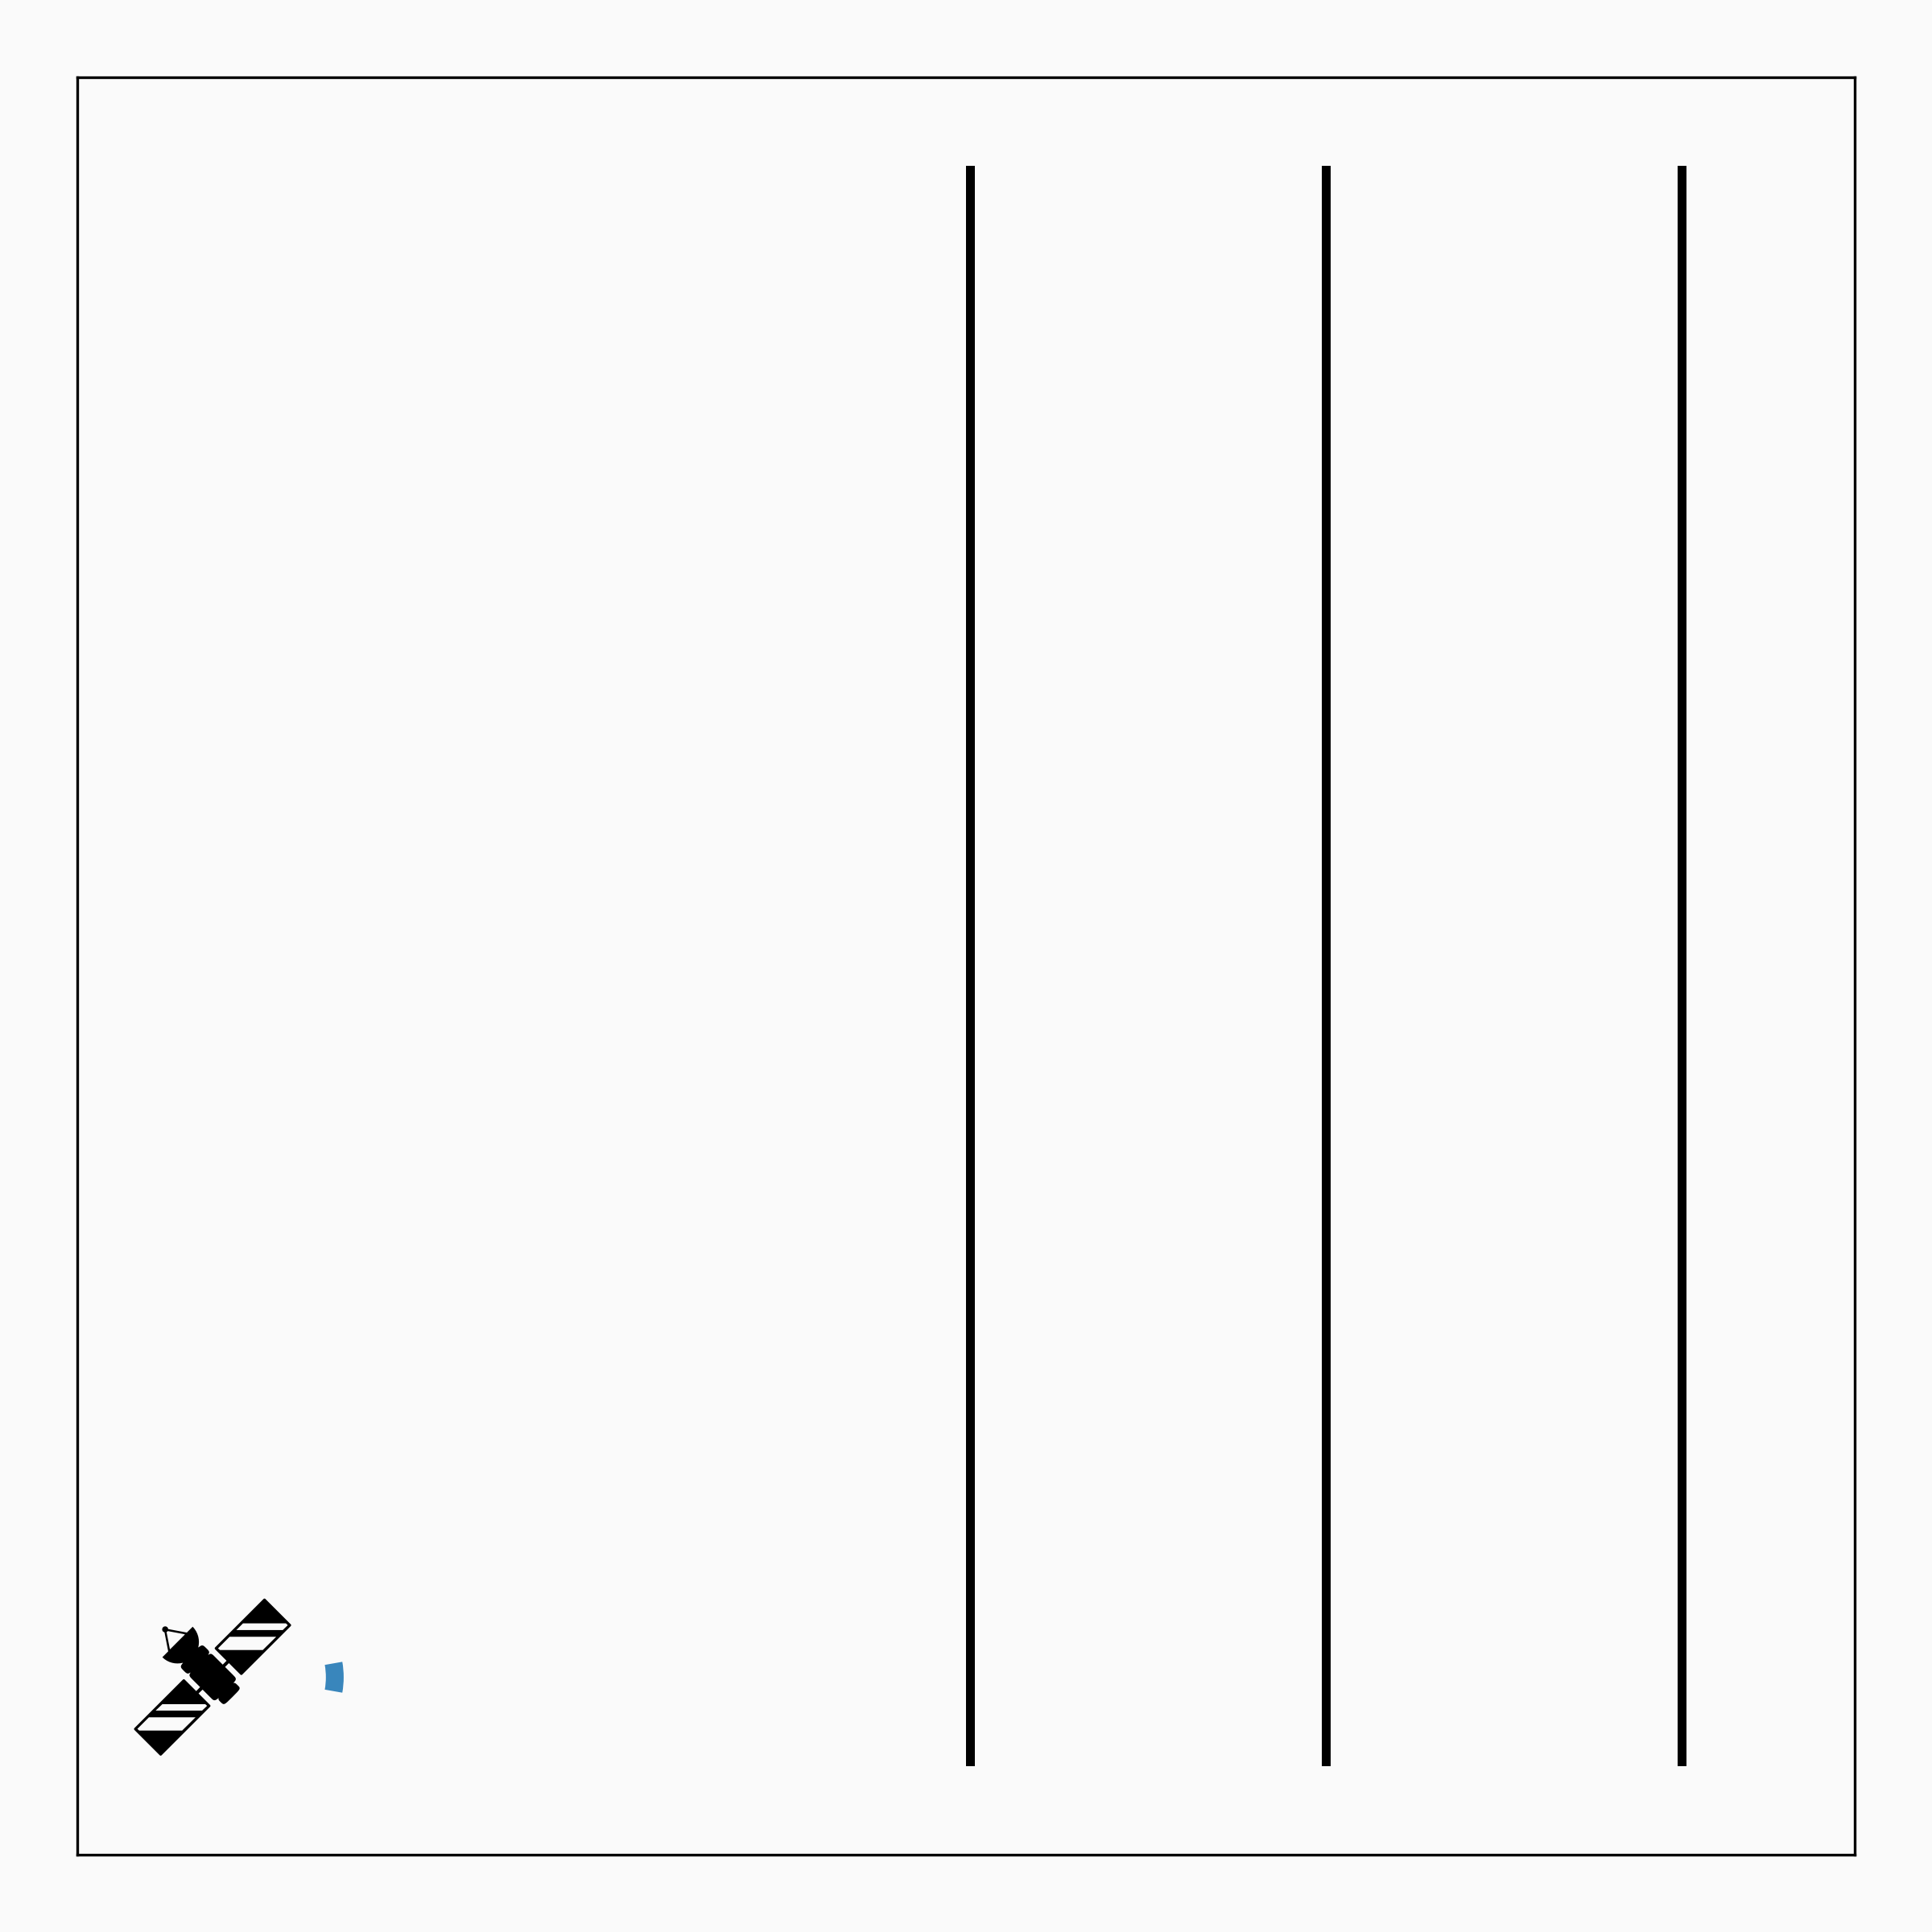
\includegraphics[width=0.45\textwidth]{fig:top.png}}{./figs/fig:top.mp4}
    \caption{Modo de adquisición TOPSAR.}
    \label{}
  \end{figure}
\end{frame}

\begin{frame}{\secname : \subsecname}
    \begin{block}{TOPSAR}
      \begin{itemize}
        \item El RADAR Va distribuyendo pulsos entre varios swaths y variando el apuntamiento en acimut para iluminar la pisada de manera mas homogénea.
        \item Gran swath.
        \item Baja resolución.
        \item Aceptable relación señal ruido y uniforme en la imagen.
        \item Buena distribución de potencia. No hay scalloping.
      \end{itemize}
    \end{block}
\end{frame}
%--- Next Frame ---%

\section{Interacción con el blanco}
\subsection{¿Que es una imagen SAR?}
\begin{frame}{\secname : \subsecname}
  \begin{columns}[t]
    \begin{column}{0.5\textwidth}
     \begin{block}{SAR}
       \begin{itemize}
         \item Una imagen SAR es un mapa de reflectividad.
         \item Indica cuanta energía es devuelta al sensor.
         \item La cantidad de energía retrodispersaada depende de la geometría del blanco y su conductividad eléctrica.
         \item Las zonas oscurar y brillantes son zonas de baja y alta reflectividad.
       \end{itemize}
     \end{block}
    \end{column}
    \begin{column}{0.5\textwidth}  %%<--- here
        \begin{figure}
          \centering
          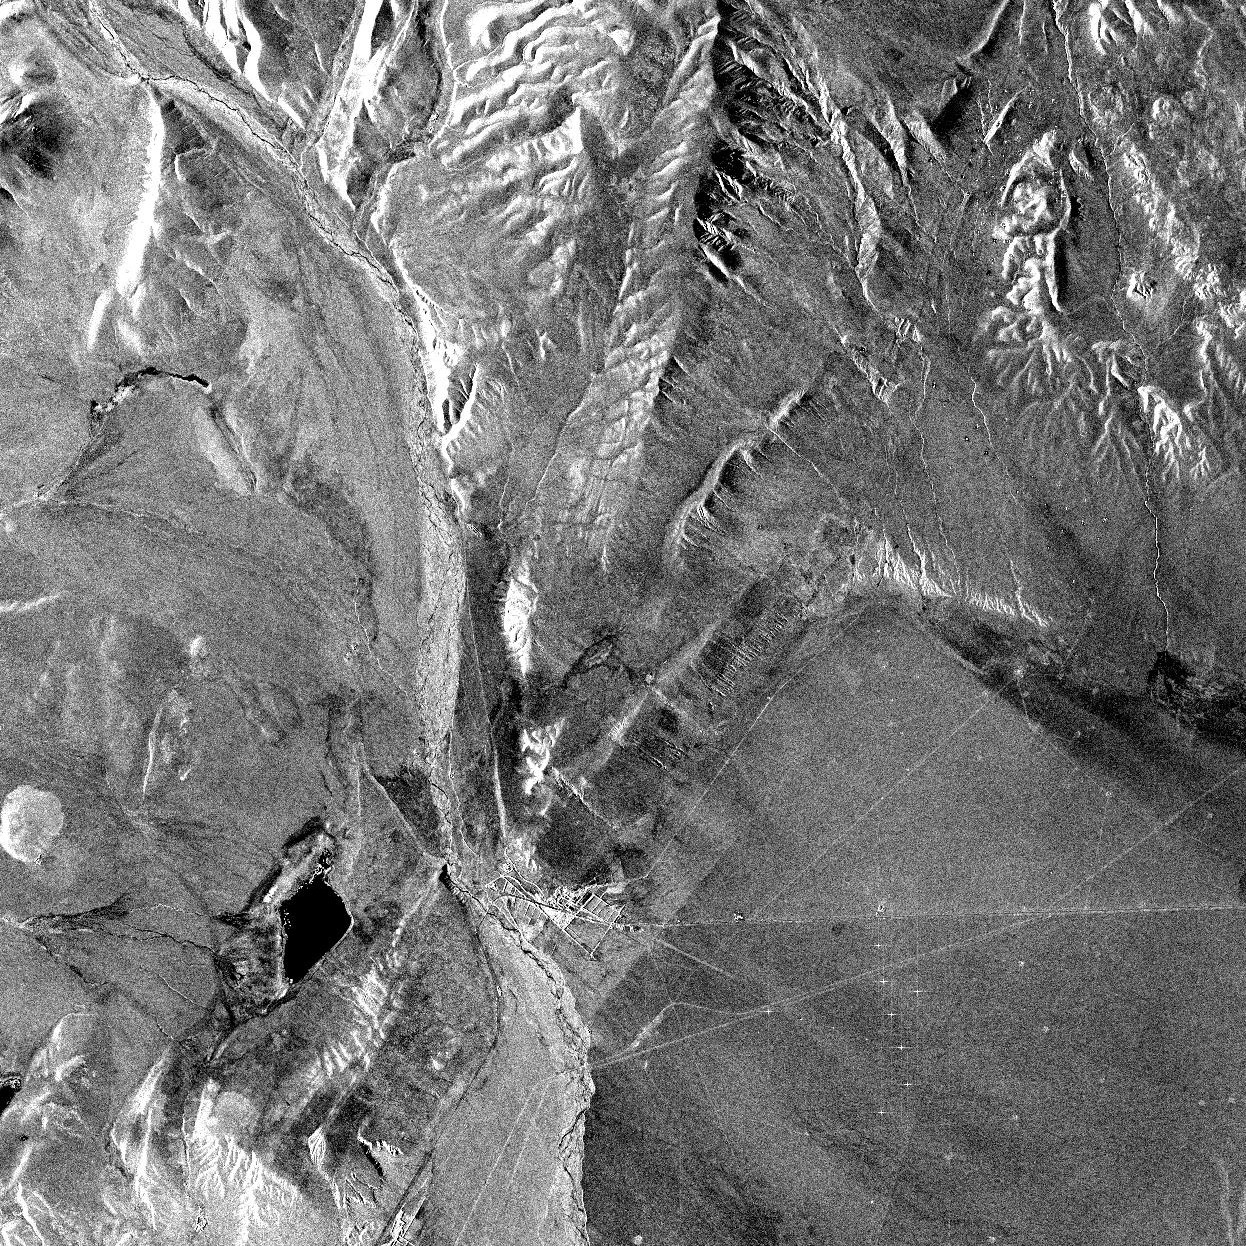
\includegraphics[width=\textwidth]{fig:sar.jpg}
          \caption{}
          \label{}
        \end{figure}
    \end{column}
    \end{columns}
\end{frame}
%--- Next Frame ---%

\begin{frame}{\secname : \subsecname}
    \begin{figure}
      \centering
      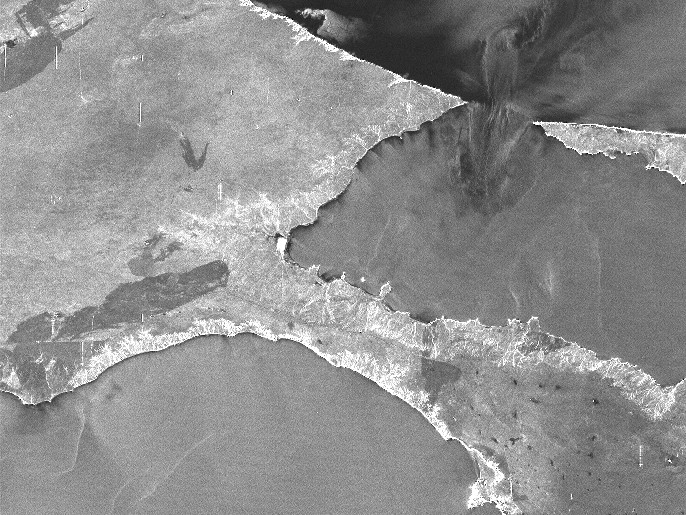
\includegraphics[width=0.6\textwidth]{fig:sar2.jpg}
      \caption{}
      \label{}
    \end{figure}
\end{frame}
%--- Next Frame ---%

\subsection{Mecanismos de scattering}

\begin{frame}{\secname : \subsecname}
    \begin{figure}
      \centering
      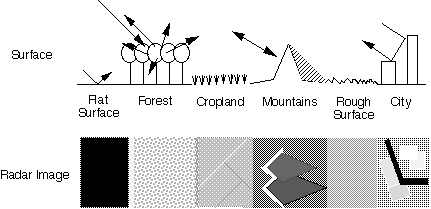
\includegraphics[width=0.6\textwidth]{fig:rebotes.png}
      \caption{}
      \label{}
    \end{figure}
\end{frame}
%--- Next Frame ---%

\begin{frame}{\secname : \subsecname}
    \begin{figure}
      \centering
      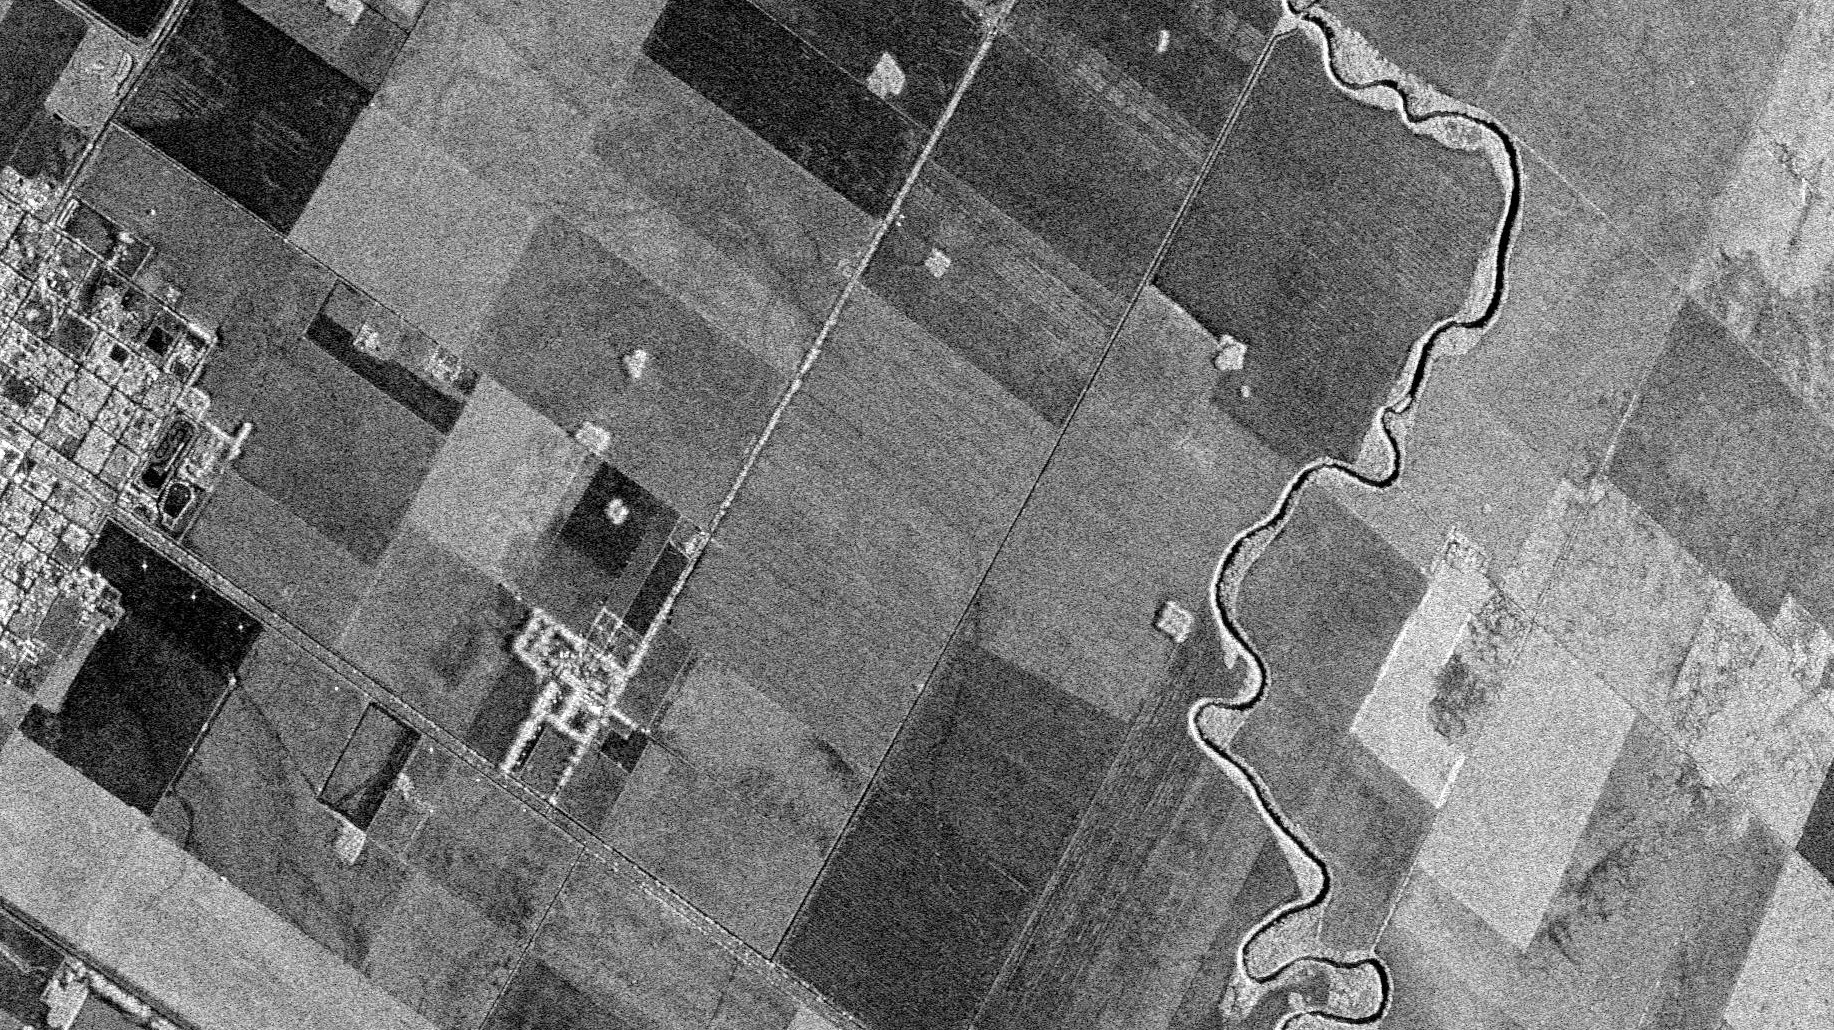
\includegraphics[width=0.6\textwidth]{fig:rebotes2.jpg}
      \caption{}
      \label{}
    \end{figure}
\end{frame}
%--- Next Frame ---%

\begin{frame}{\secname : \subsecname}
    \begin{figure}
      \centering
      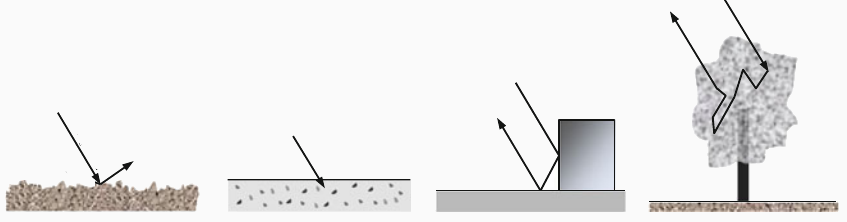
\includegraphics[width=0.5\textwidth]{fig:interacciones.png}
      \caption{}
      \label{}
    \end{figure}
\end{frame}
%--- Next Frame ---%

\begin{frame}{\secname : \subsecname}
    \begin{figure}
    \centering
\subfloat[Banda C ($5.7cm$)]{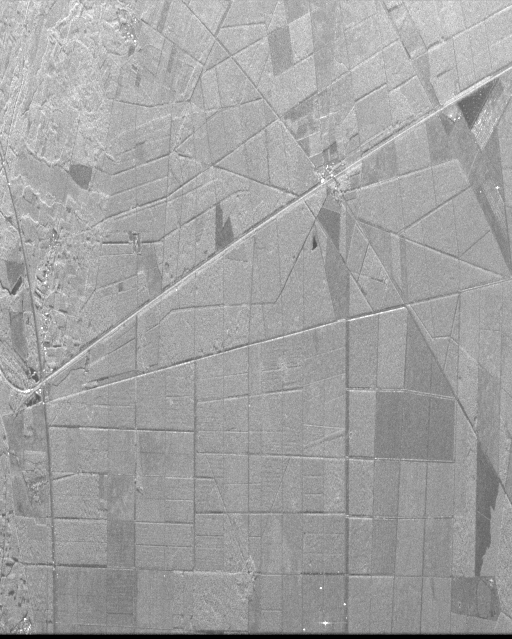
\includegraphics[width=0.2\textwidth]{fig:C.png}}\hspace{1cm}
\subfloat[Banda L ($24cm$)]{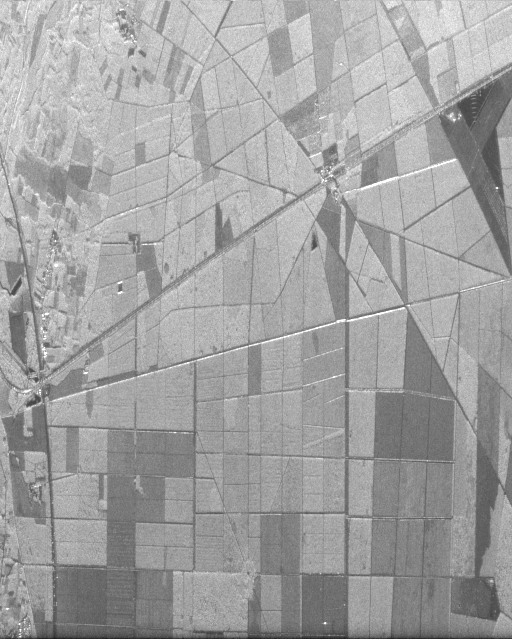
\includegraphics[width=0.2\textwidth]{fig:L.png}}\hspace{1cm}
\subfloat[Banda P ($68cm$)]{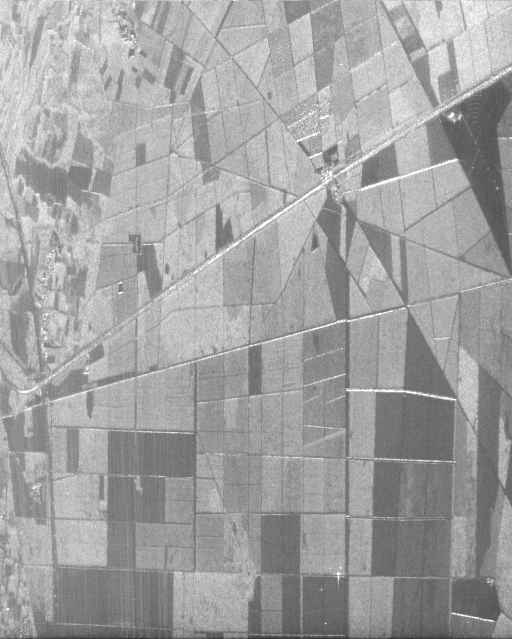
\includegraphics[width=0.2\textwidth]{fig:P.png}}
    \end{figure}
\end{frame}
%--- Next Frame ---%

\section{Formación de imágenes satelitales}
\subsection{Partes de una imagen}
%--- Next Frame ---%

\begin{frame}{}
\begin{block}{Píxel}
  Un píxel es el mínimo elemento de una imagen. 
\end{block}\pause
\begin{block}{Banda}
  Una imagen digital es un agrupamiento de píxeles en dos dimensiones. 
\end{block}
\end{frame}

%--- Next Frame ---%
\begin{frame}{}
  \begin{figure}
    \centering
    \movie[width = 0.8\textwidth,loop,autostart]{\centering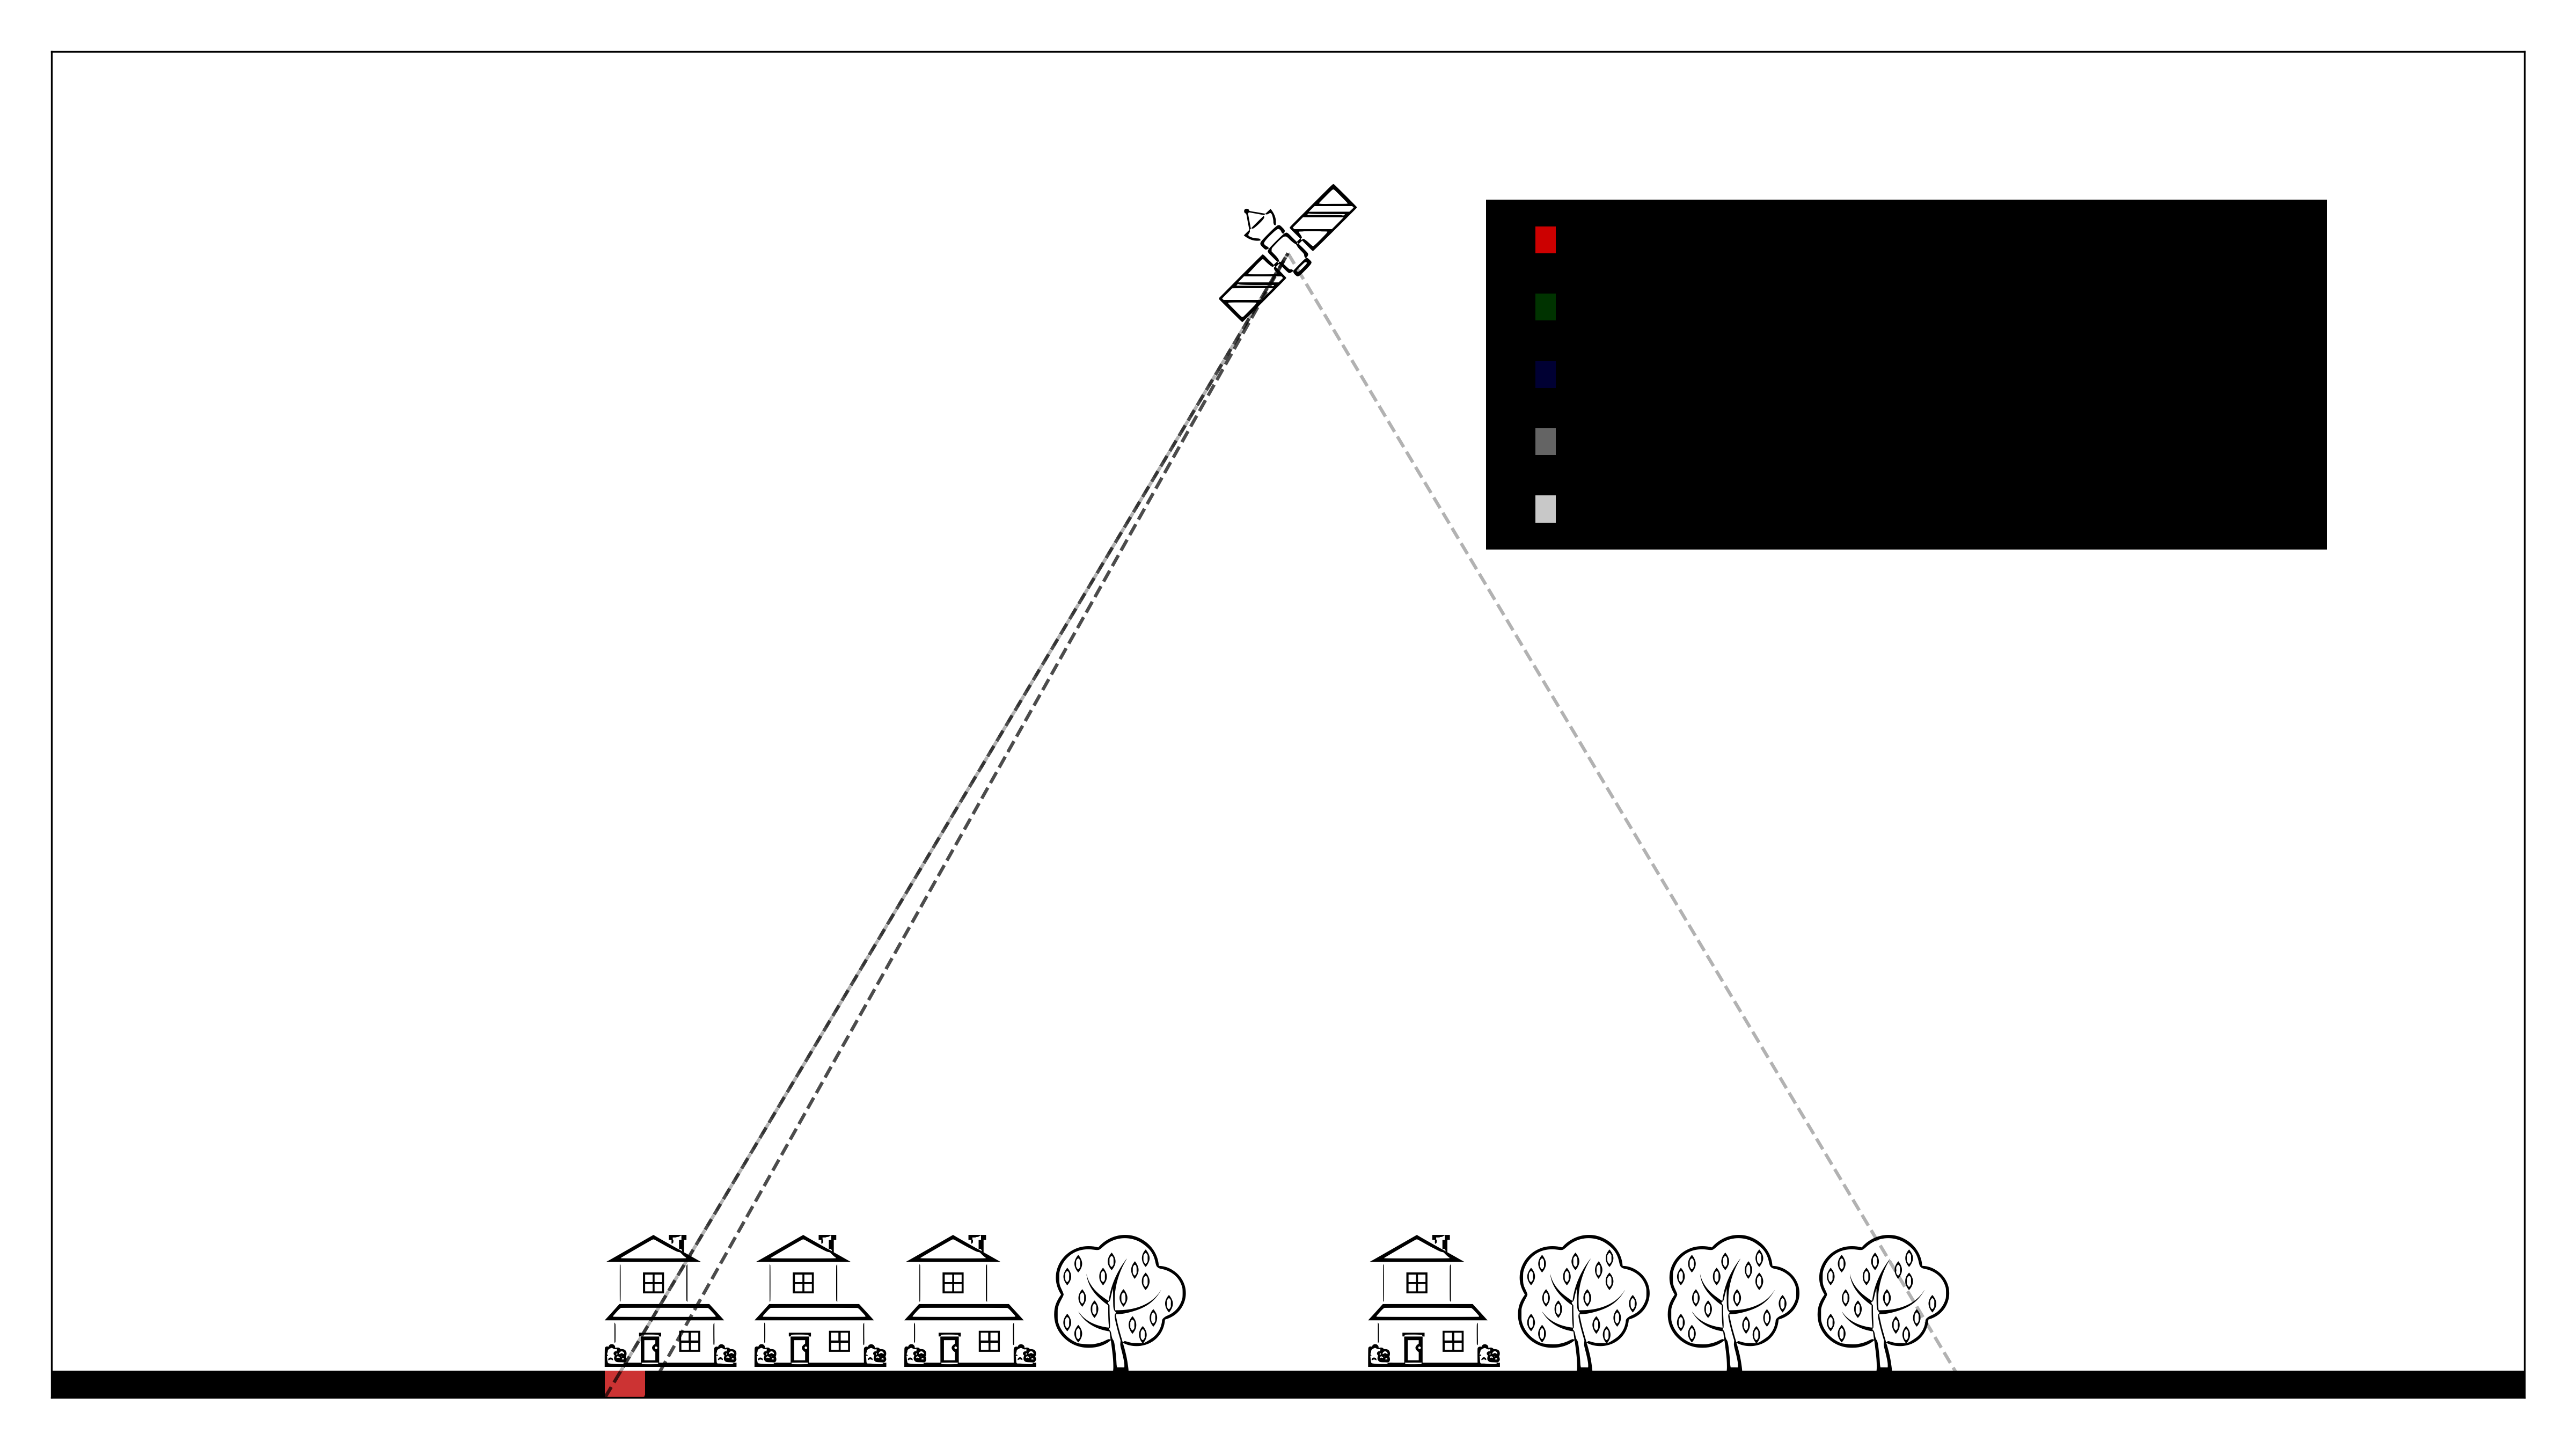
\includegraphics[width=0.8\textwidth]{fig:fimagen.png}}{./figs/fig:fimagen.mp4}
    \caption{Formación de una imagen.}
    \label{}
  \end{figure}
\end{frame}
% modificar el video, no me cierra nada, es bastante confuso, o mejorar o cambiar.



\begin{frame}{}
  \begin{block}{Imagen}
    En general vamos a hablar de una imagen, o un raster, como el conjunto de bandas.
  \end{block}
\end{frame}
%--- Next Frame ---%

\subsection{Resolución espectral y radiométrica}

\begin{frame}{}
  \begin{block}{Radiometría}
    Resolución radiométrica
  \end{block}
\end{frame}
%--- Next Frame ---%

\begin{frame}{}
  \begin{block}{8 bits}
   \begin{equation}
            2^8 = 0-255
        \end{equation}
  \end{block}
\end{frame}

%--- Next Frame ---%

\begin{frame}{}
  \begin{figure}
    \centering
    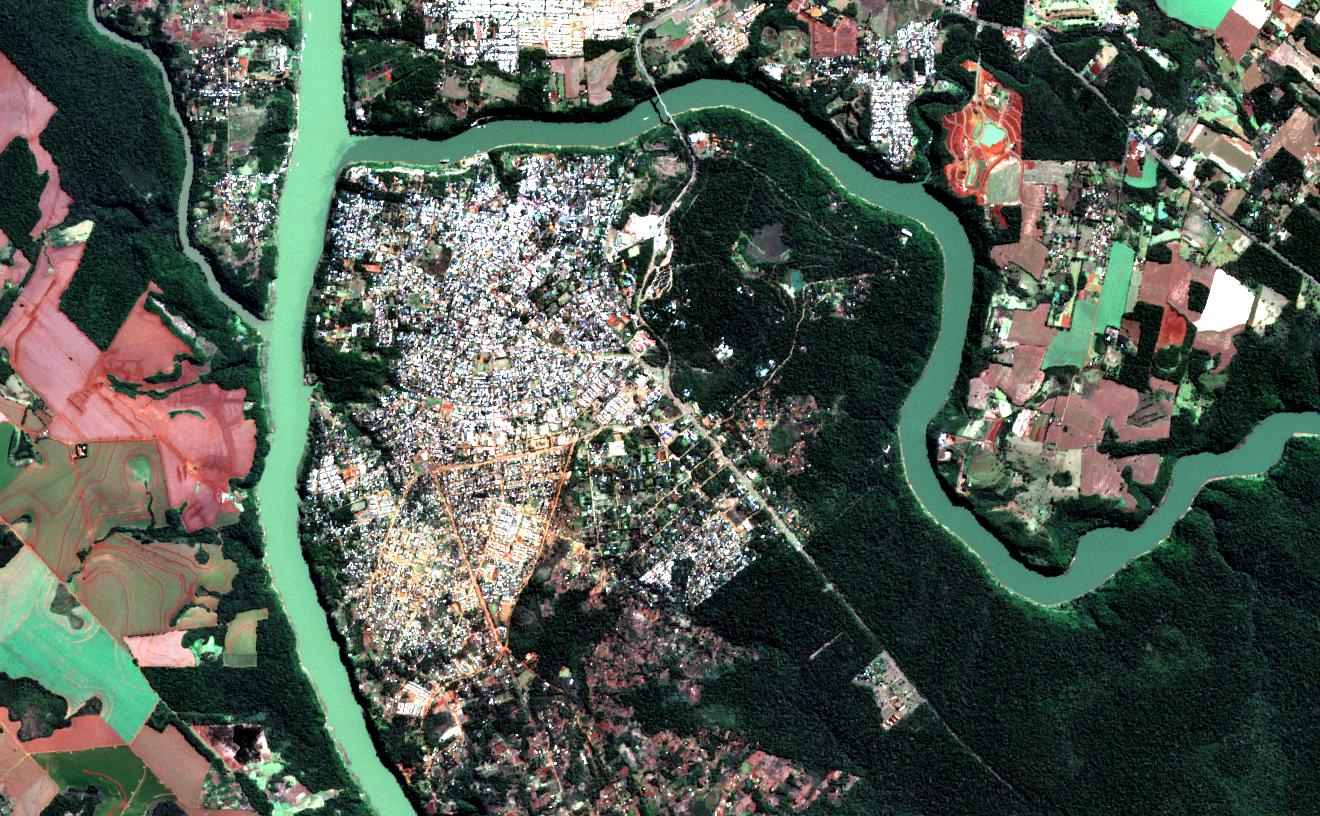
\includegraphics[width=0.7\textwidth]{fig:8bit.jpg}
    \caption{Imagen con resolución radiométrica de 8bit.}
    \label{}
  \end{figure}
\end{frame}
%--- Next Frame ---%


\begin{frame}{}
  \begin{block}{4 bits}
   \begin{equation}
            2^4 = 0-15
        \end{equation}
  \end{block}
\end{frame}

%--- Next Frame ---%

\begin{frame}{}
  \begin{figure}
    \centering
    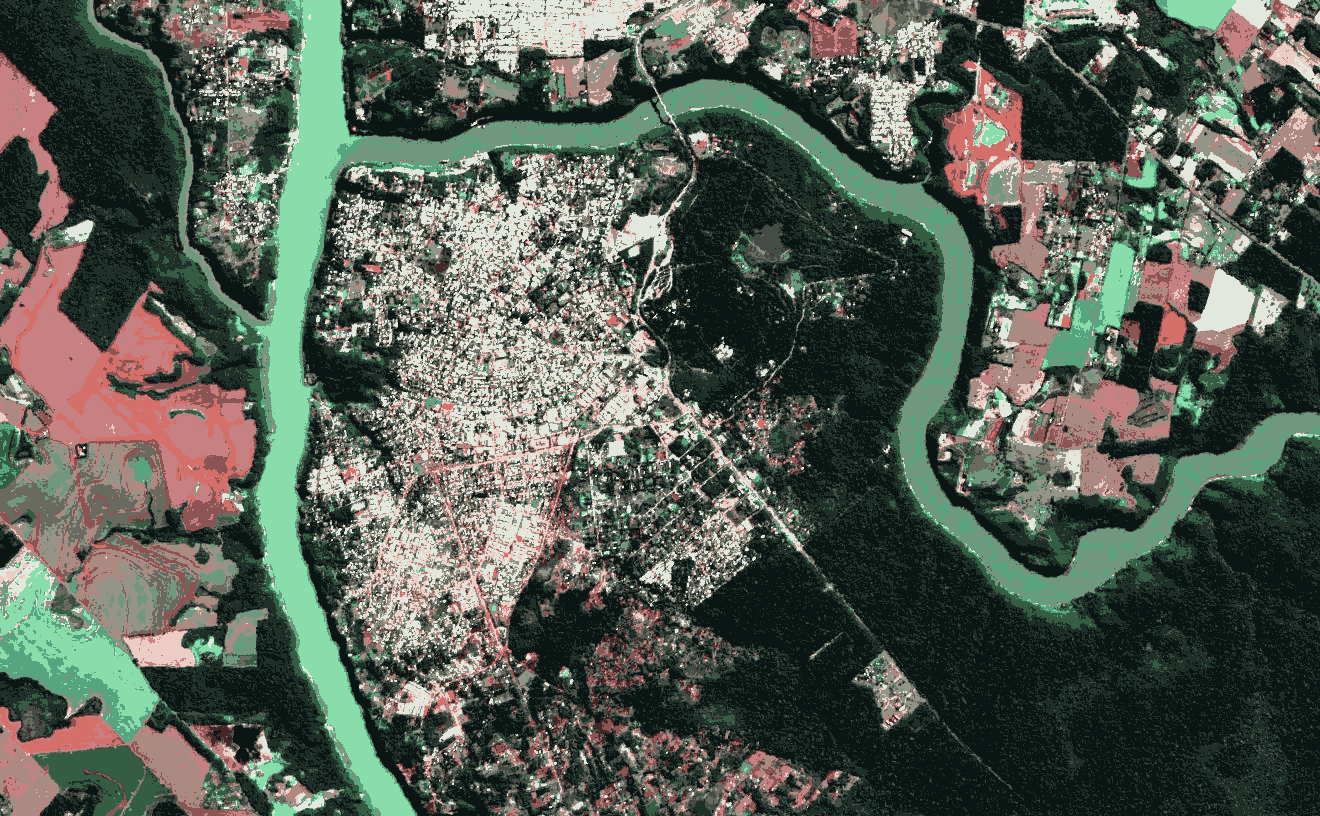
\includegraphics[width=0.7\textwidth]{fig:4bit.jpg}
    \caption{Imagen con resolución radiométrica de 4bit.}
    \label{}
  \end{figure}
\end{frame}
%--- Next Frame ---%


\begin{frame}{}
  \begin{block}{2 bits}
   \begin{equation}
            2^2 = 0-3
        \end{equation}
  \end{block}
\end{frame}

%--- Next Frame ---%

\begin{frame}{}
  \begin{figure}
    \centering
    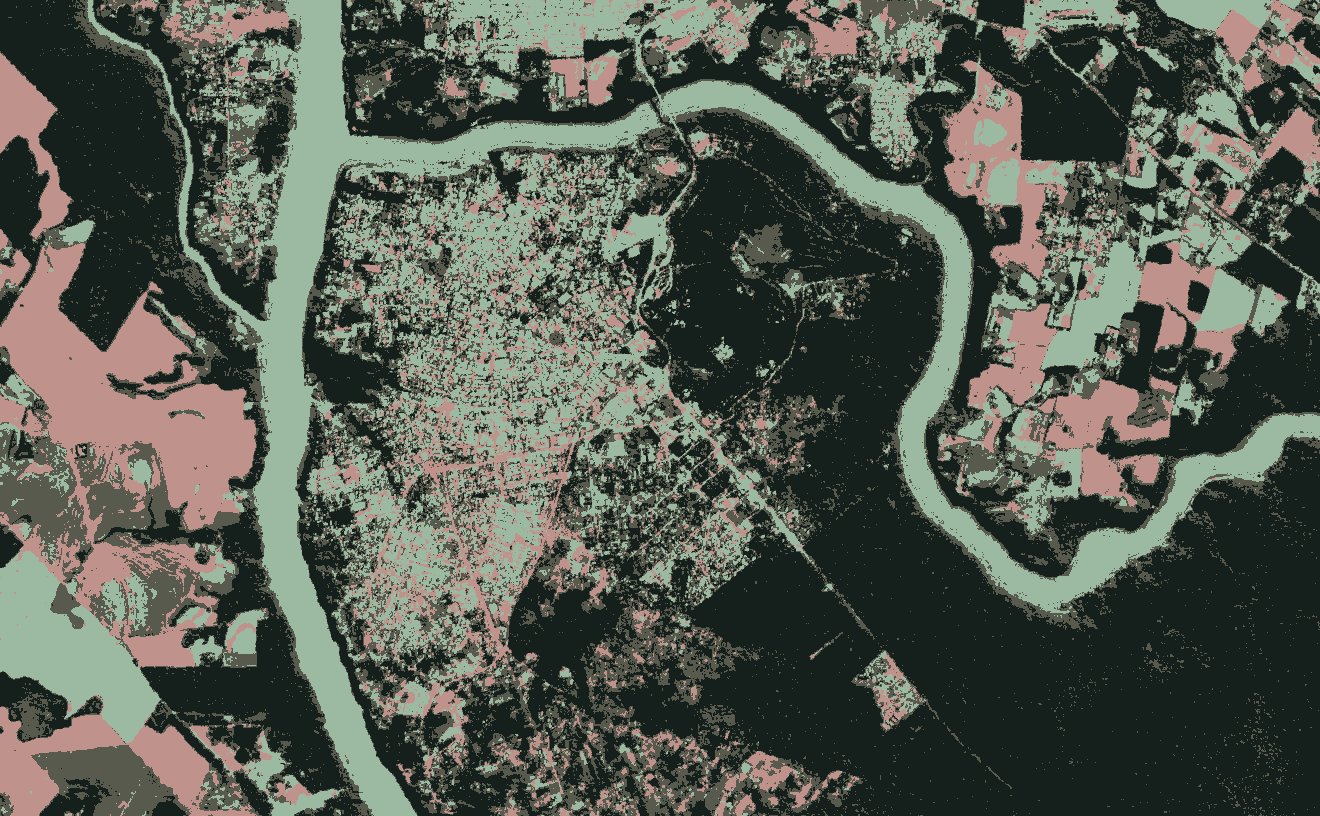
\includegraphics[width=0.7\textwidth]{fig:2bit.jpg}
    \caption{Imagen con resolución radiométrica de 2bit.}
    \label{}
  \end{figure}
\end{frame}
%--- Next Frame ---%



%--- Next Frame ---%

\begin{frame}{}
  \begin{block}{1 bits}
   \begin{equation}
            2^1 = 0-1
        \end{equation}
  \end{block}
\end{frame}

%--- Next Frame ---%

\begin{frame}{}
  \begin{figure}
    \centering
    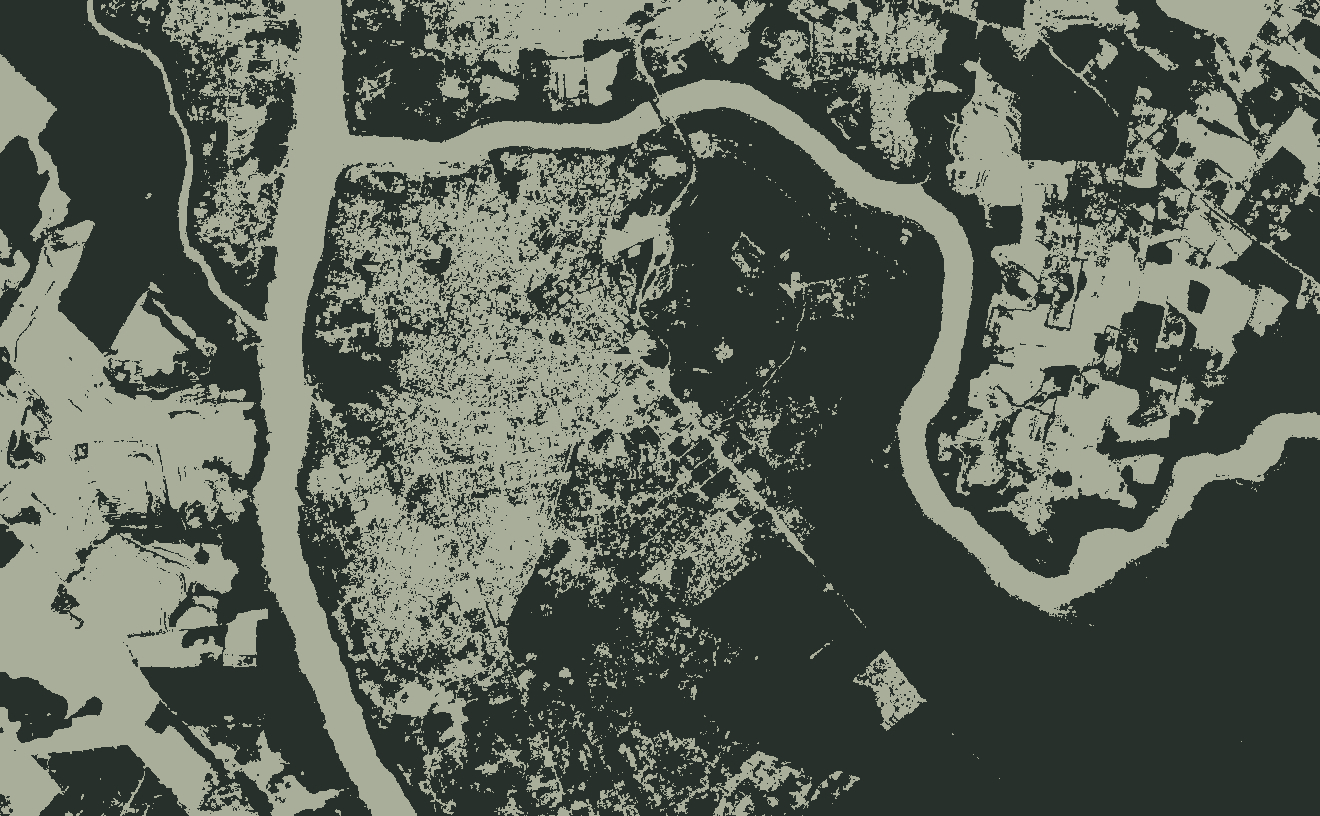
\includegraphics[width=0.7\textwidth]{fig:1bit.jpg}
    \caption{Imagen con resolución radiométrica de 1bit.}
    \label{}
  \end{figure}
\end{frame}
%--- Next Frame ---%



\begin{frame}{}
    \begin{block}{Resolución espectral}
        Es el número de y tamaño de intervalos de un rango de lon
    \end{block}
\end{frame}
%--- Next Frame ---%

\begin{frame}{}
  \begin{figure}
    \centering
    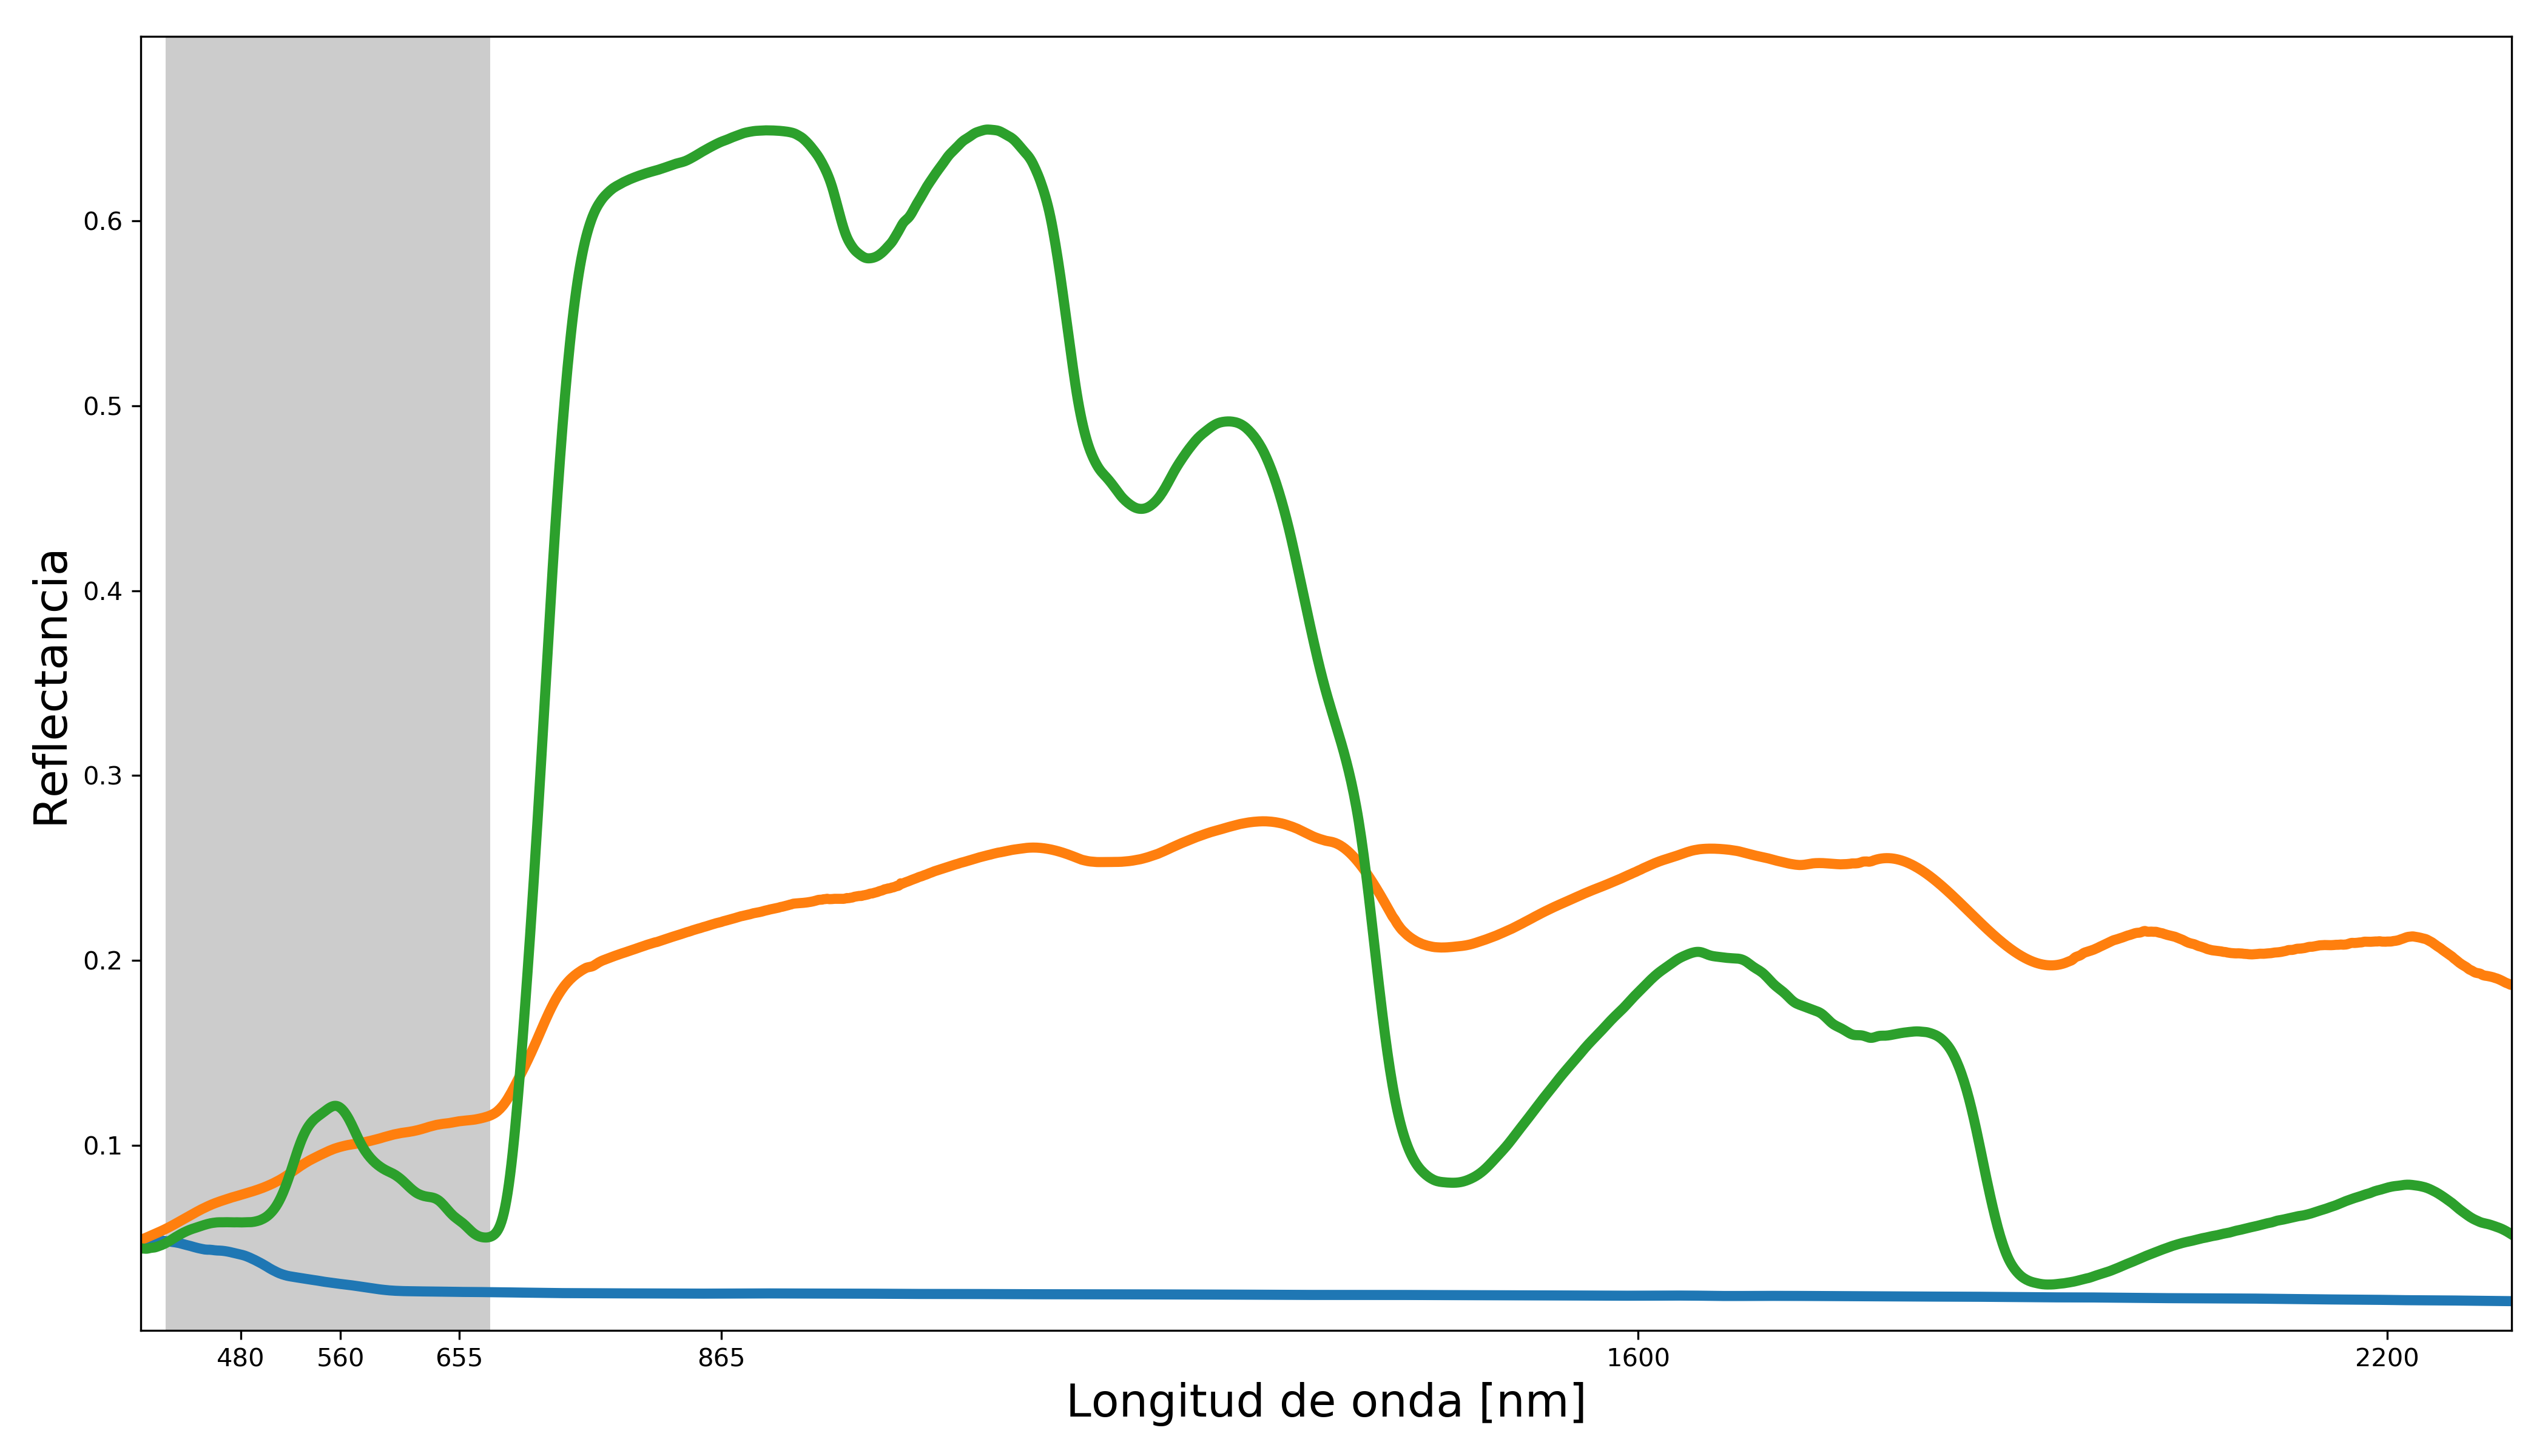
\includegraphics[width=0.8\textwidth]{fig:eslo.png}
    \caption{Resolución espectral sobre la firma espectral.}
    \label{}
  \end{figure}
\end{frame}
%--- Next Frame ---%

\begin{frame}{}
  \begin{figure}
    \centering
    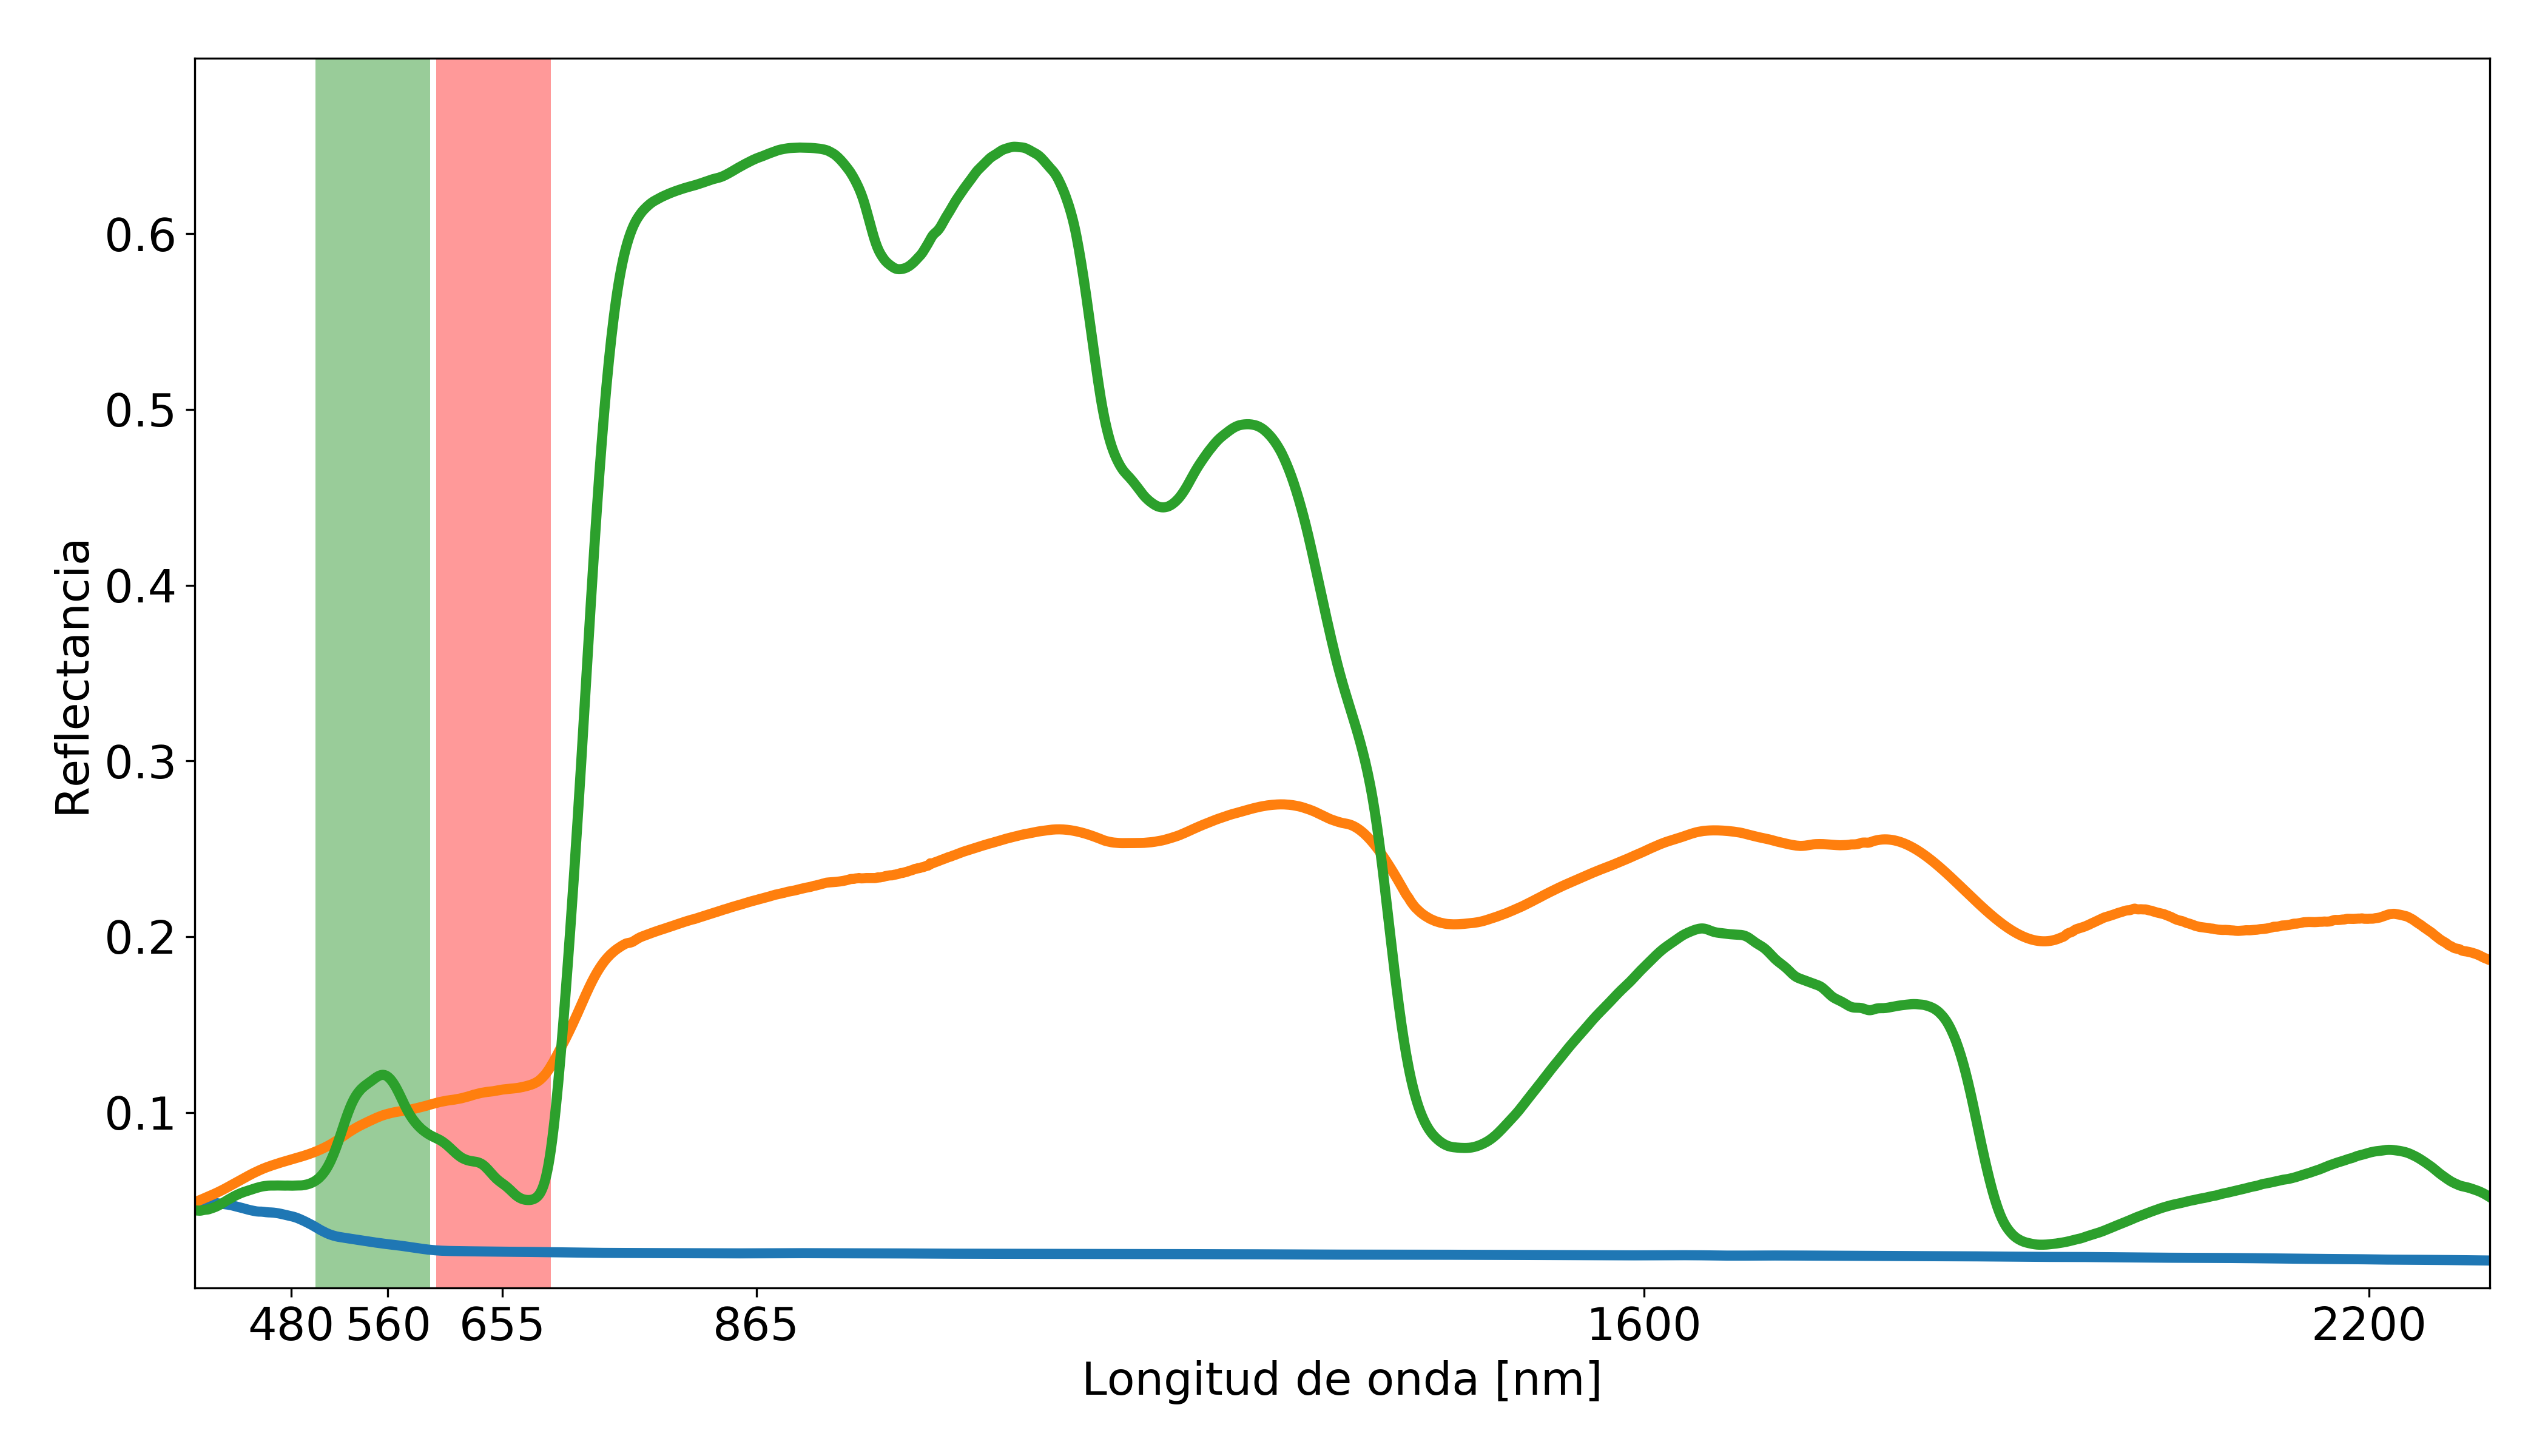
\includegraphics[width=0.8\textwidth]{fig:eshi.png}
    \caption{Resolución espectral sobre la firma espectral.}
    \label{}
  \end{figure}
\end{frame}
%--- Next Frame ---%

\begin{frame}{}
    \begin{block}{Definición}
        Es la capacidad del sensor de distinguir regiones del espectro electromagnético.
    \end{block}
\end{frame}
%--- Next Frame ---%

%\subsection{Proyección sobre el terreno}

%\begin{frame}{}
%  \begin{figure}
%    \centering
    %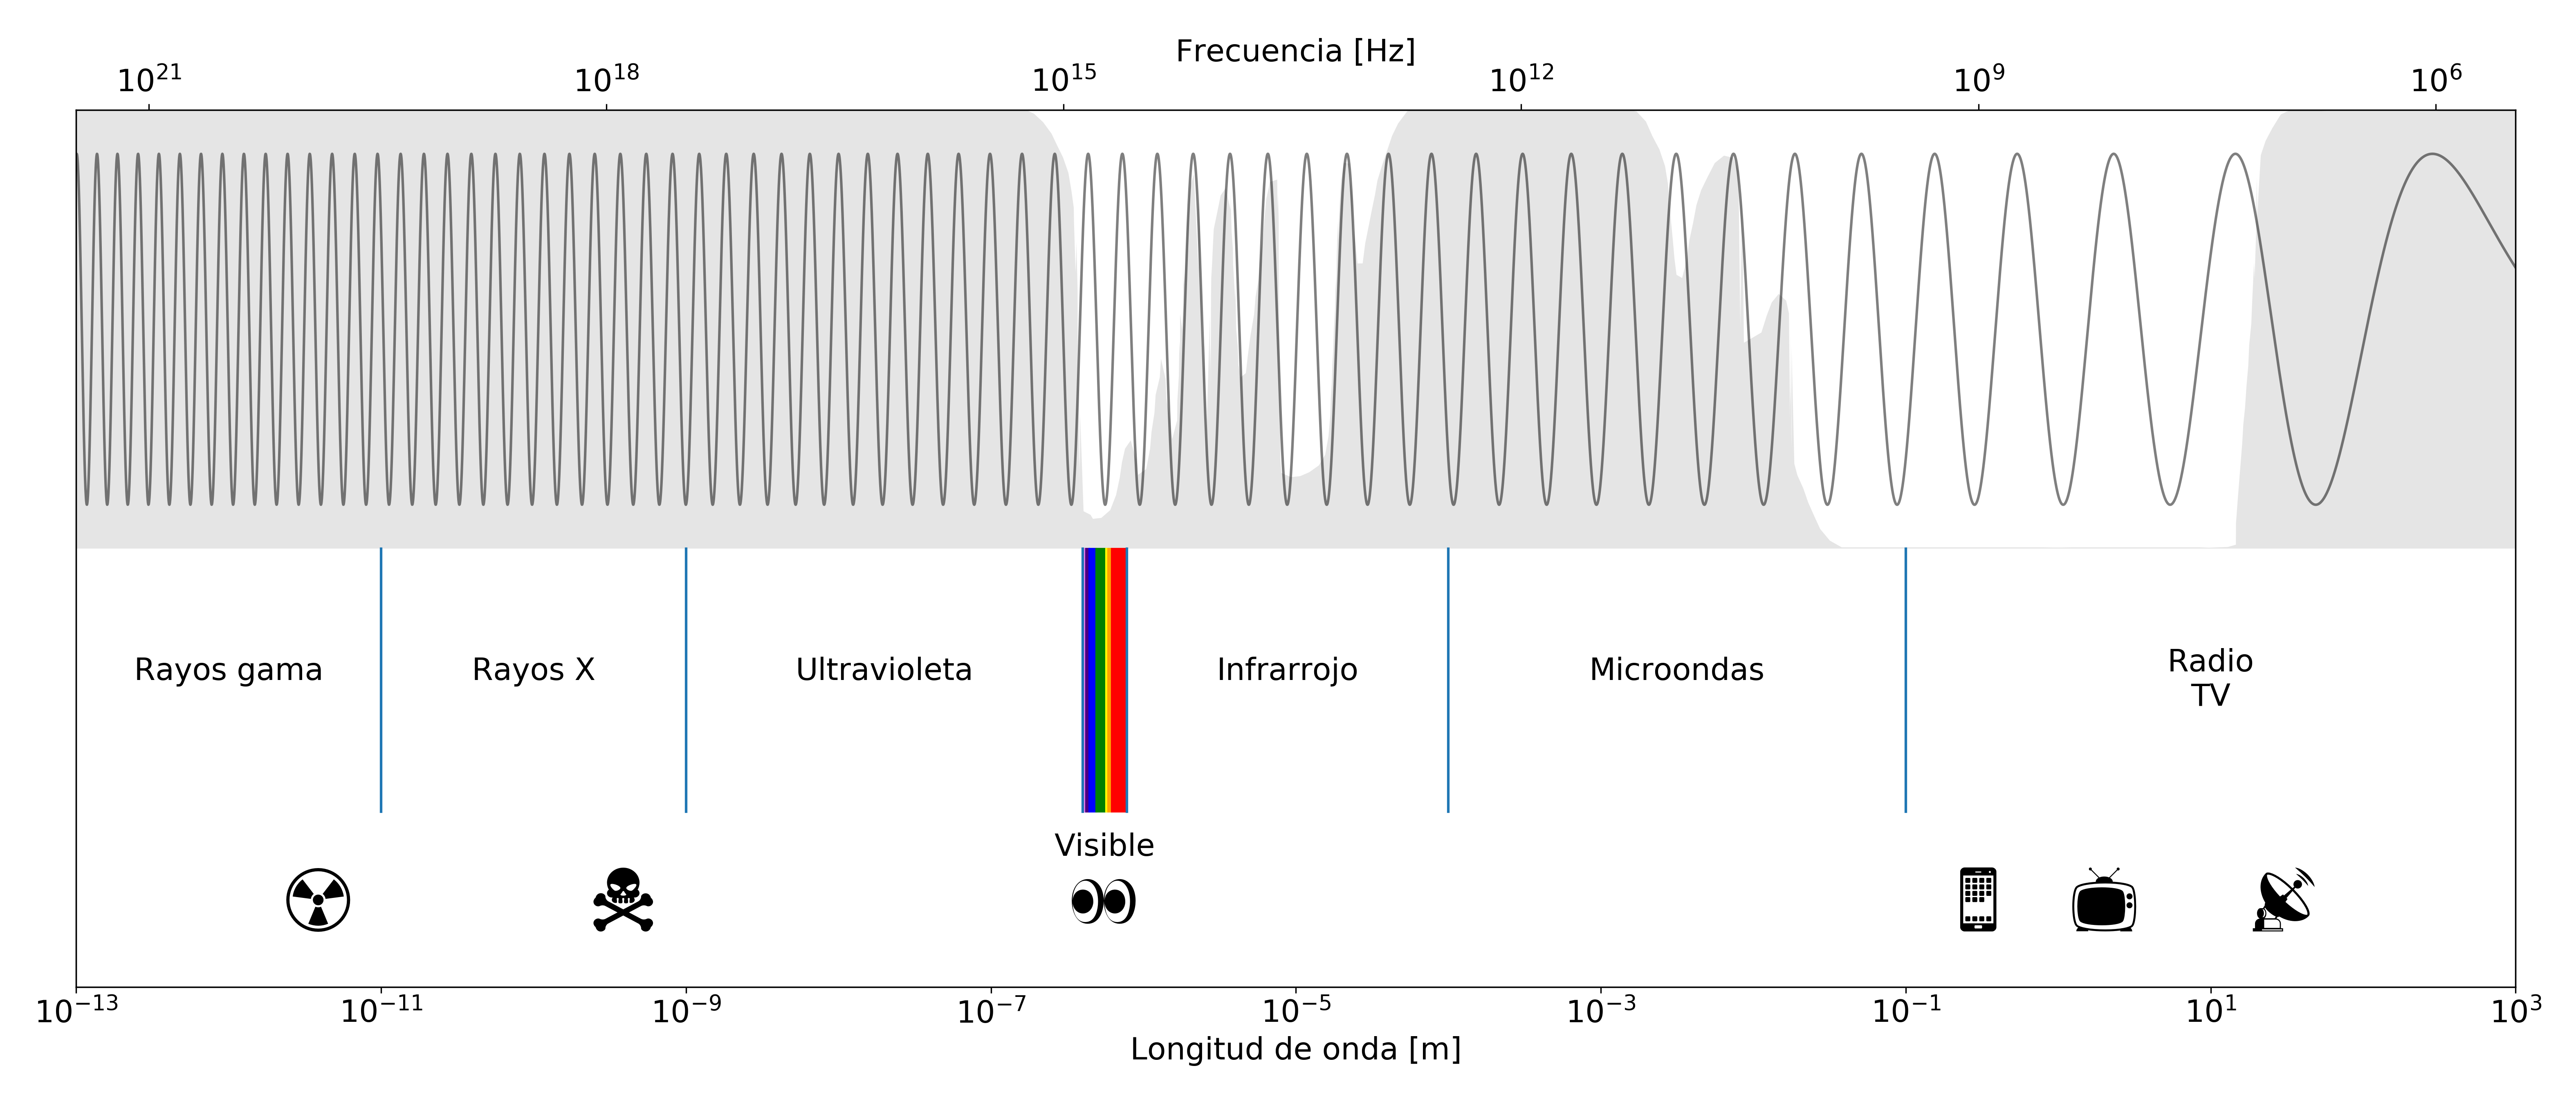
\includegraphics[width=\textwidth]{fig:espectro.png}
%    \caption{Asignación de coordenadas a píxeles.}
%    \label{}
%  \end{figure}
%\end{frame}
%--- Next Frame ---%

%\begin{frame}{}
%  \begin{figure}
%    \centering
    %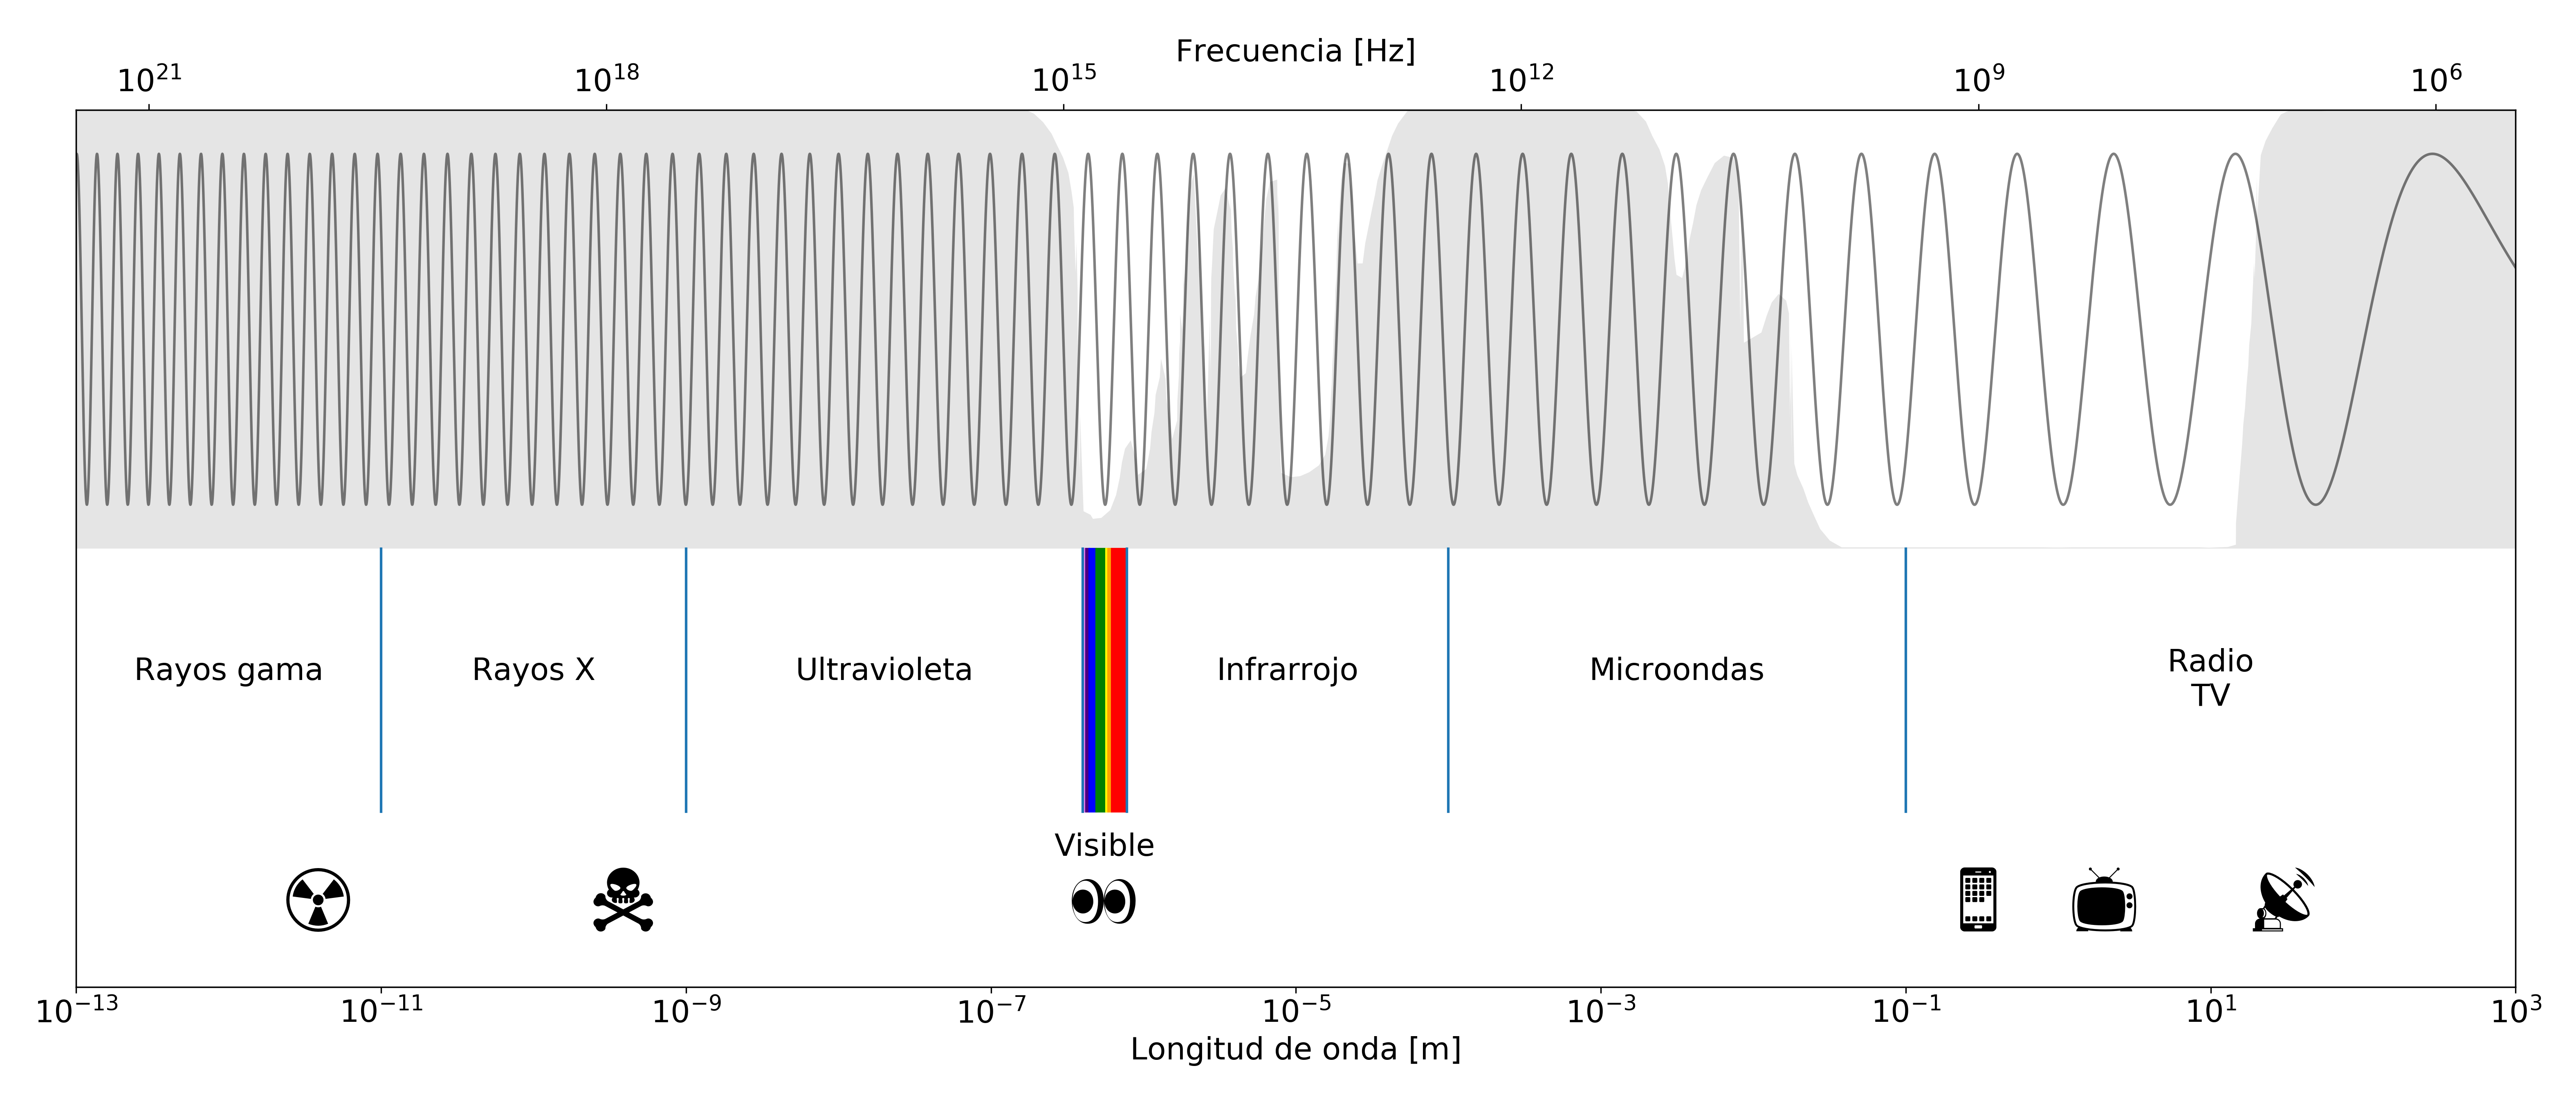
\includegraphics[width=\textwidth]{fig:espectro.png}
%    \caption{Proyección de una esfera en un plano.}
%    \label{}
%  \end{figure}
%\end{frame}
%--- Next Frame ---%

%\begin{frame}{}
%  \begin{figure}
%    \centering
    %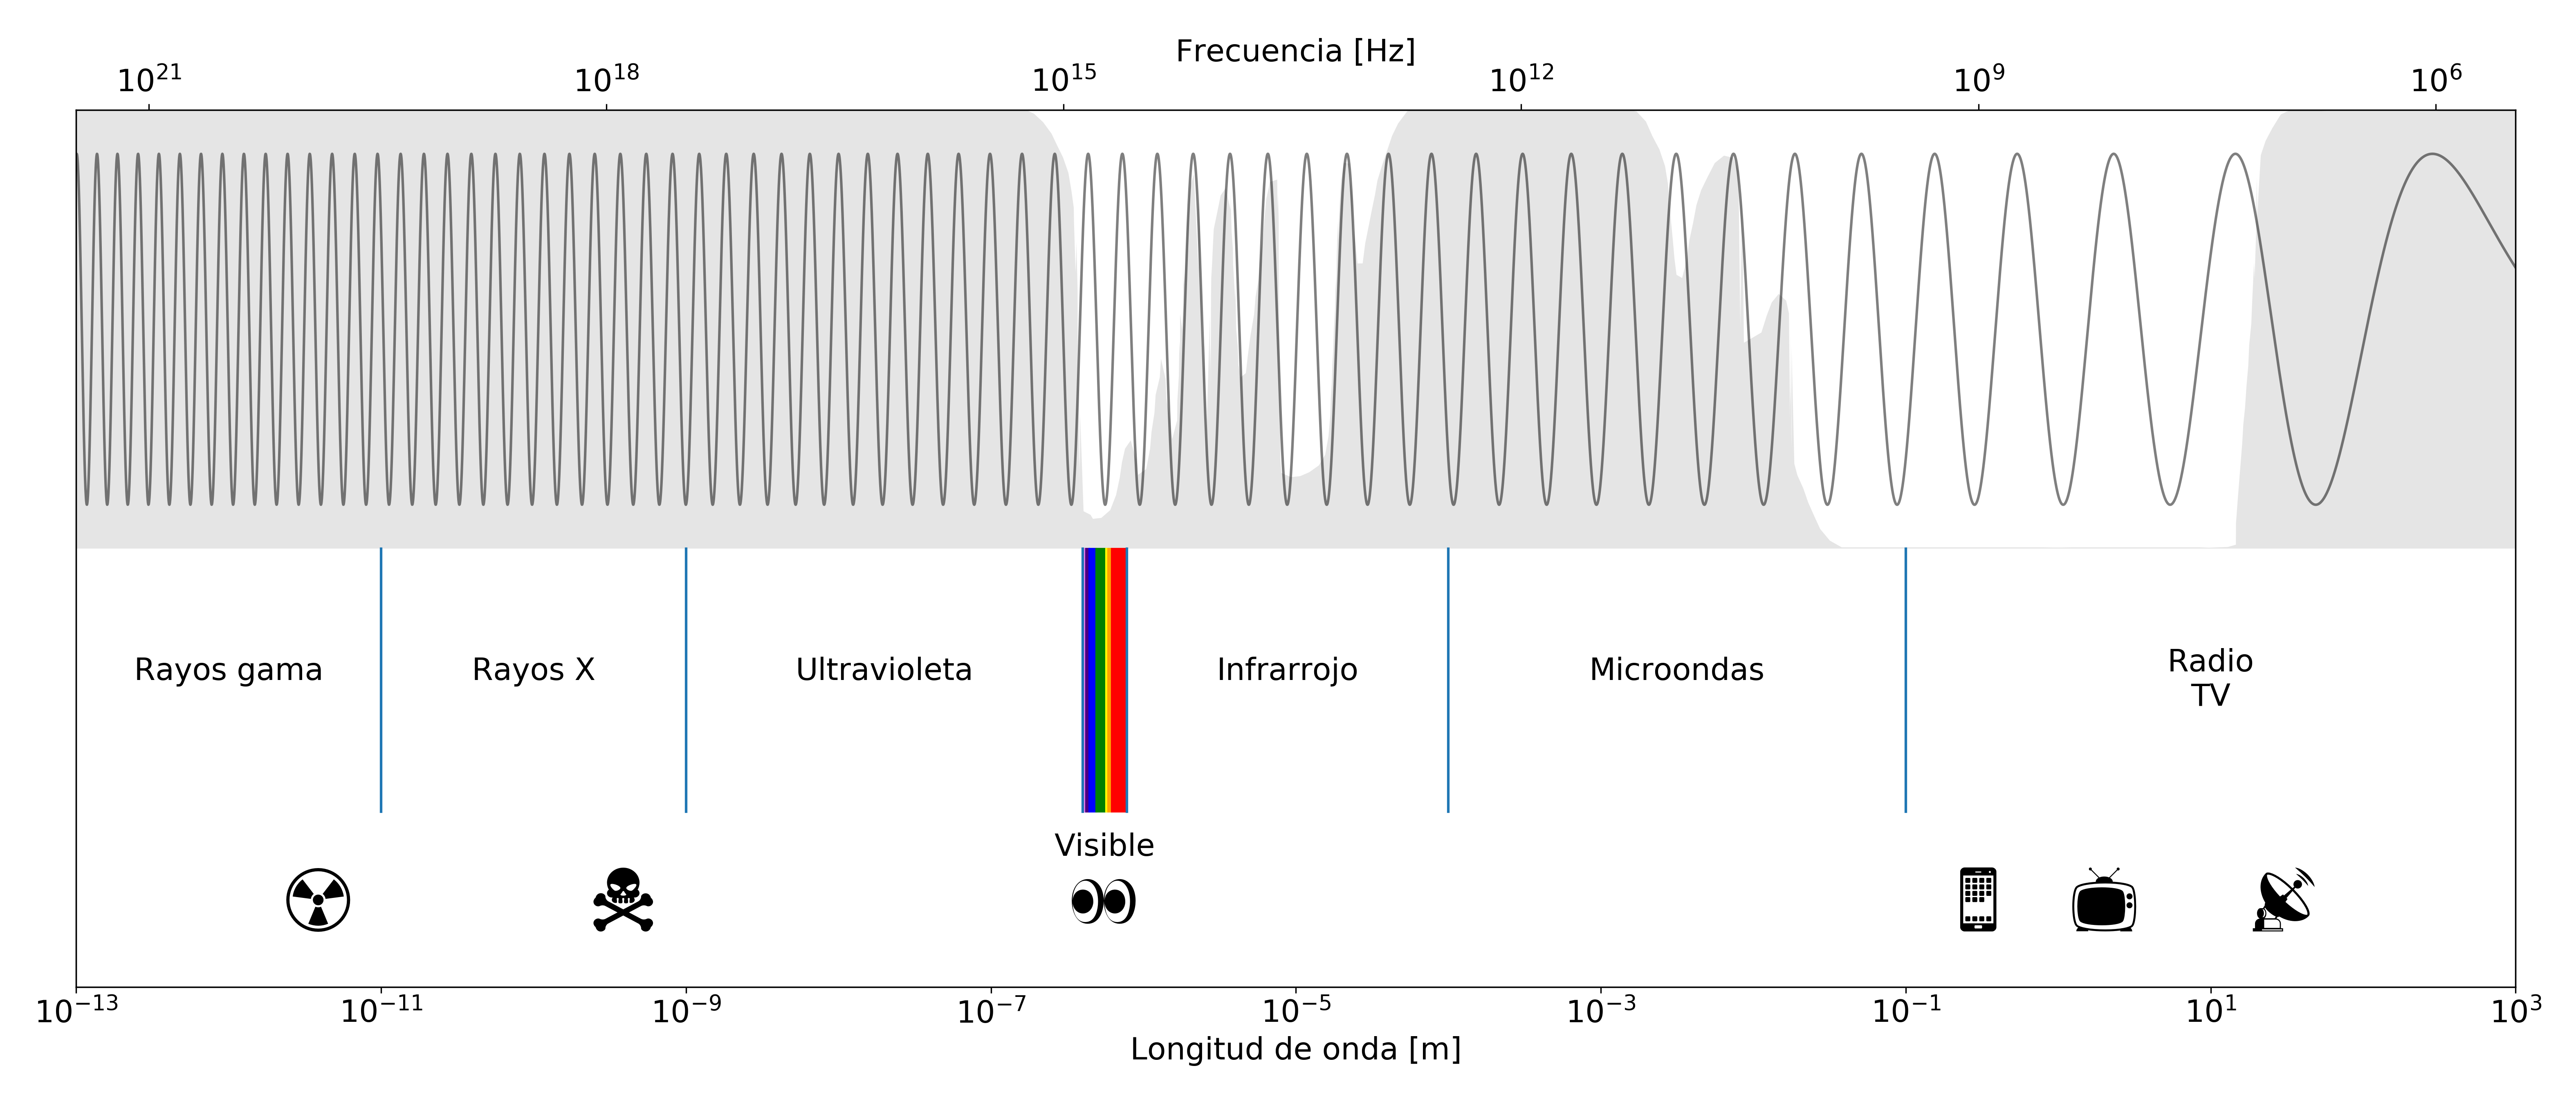
\includegraphics[width=\textwidth]{fig:espectro.png}
%    \caption{Métodos de interpolación.}
%    \label{}
%  \end{figure}
%\end{frame}
%--- Next Frame ---%

%\begin{frame}{}
%  \begin{figure}
%    \centering
%    %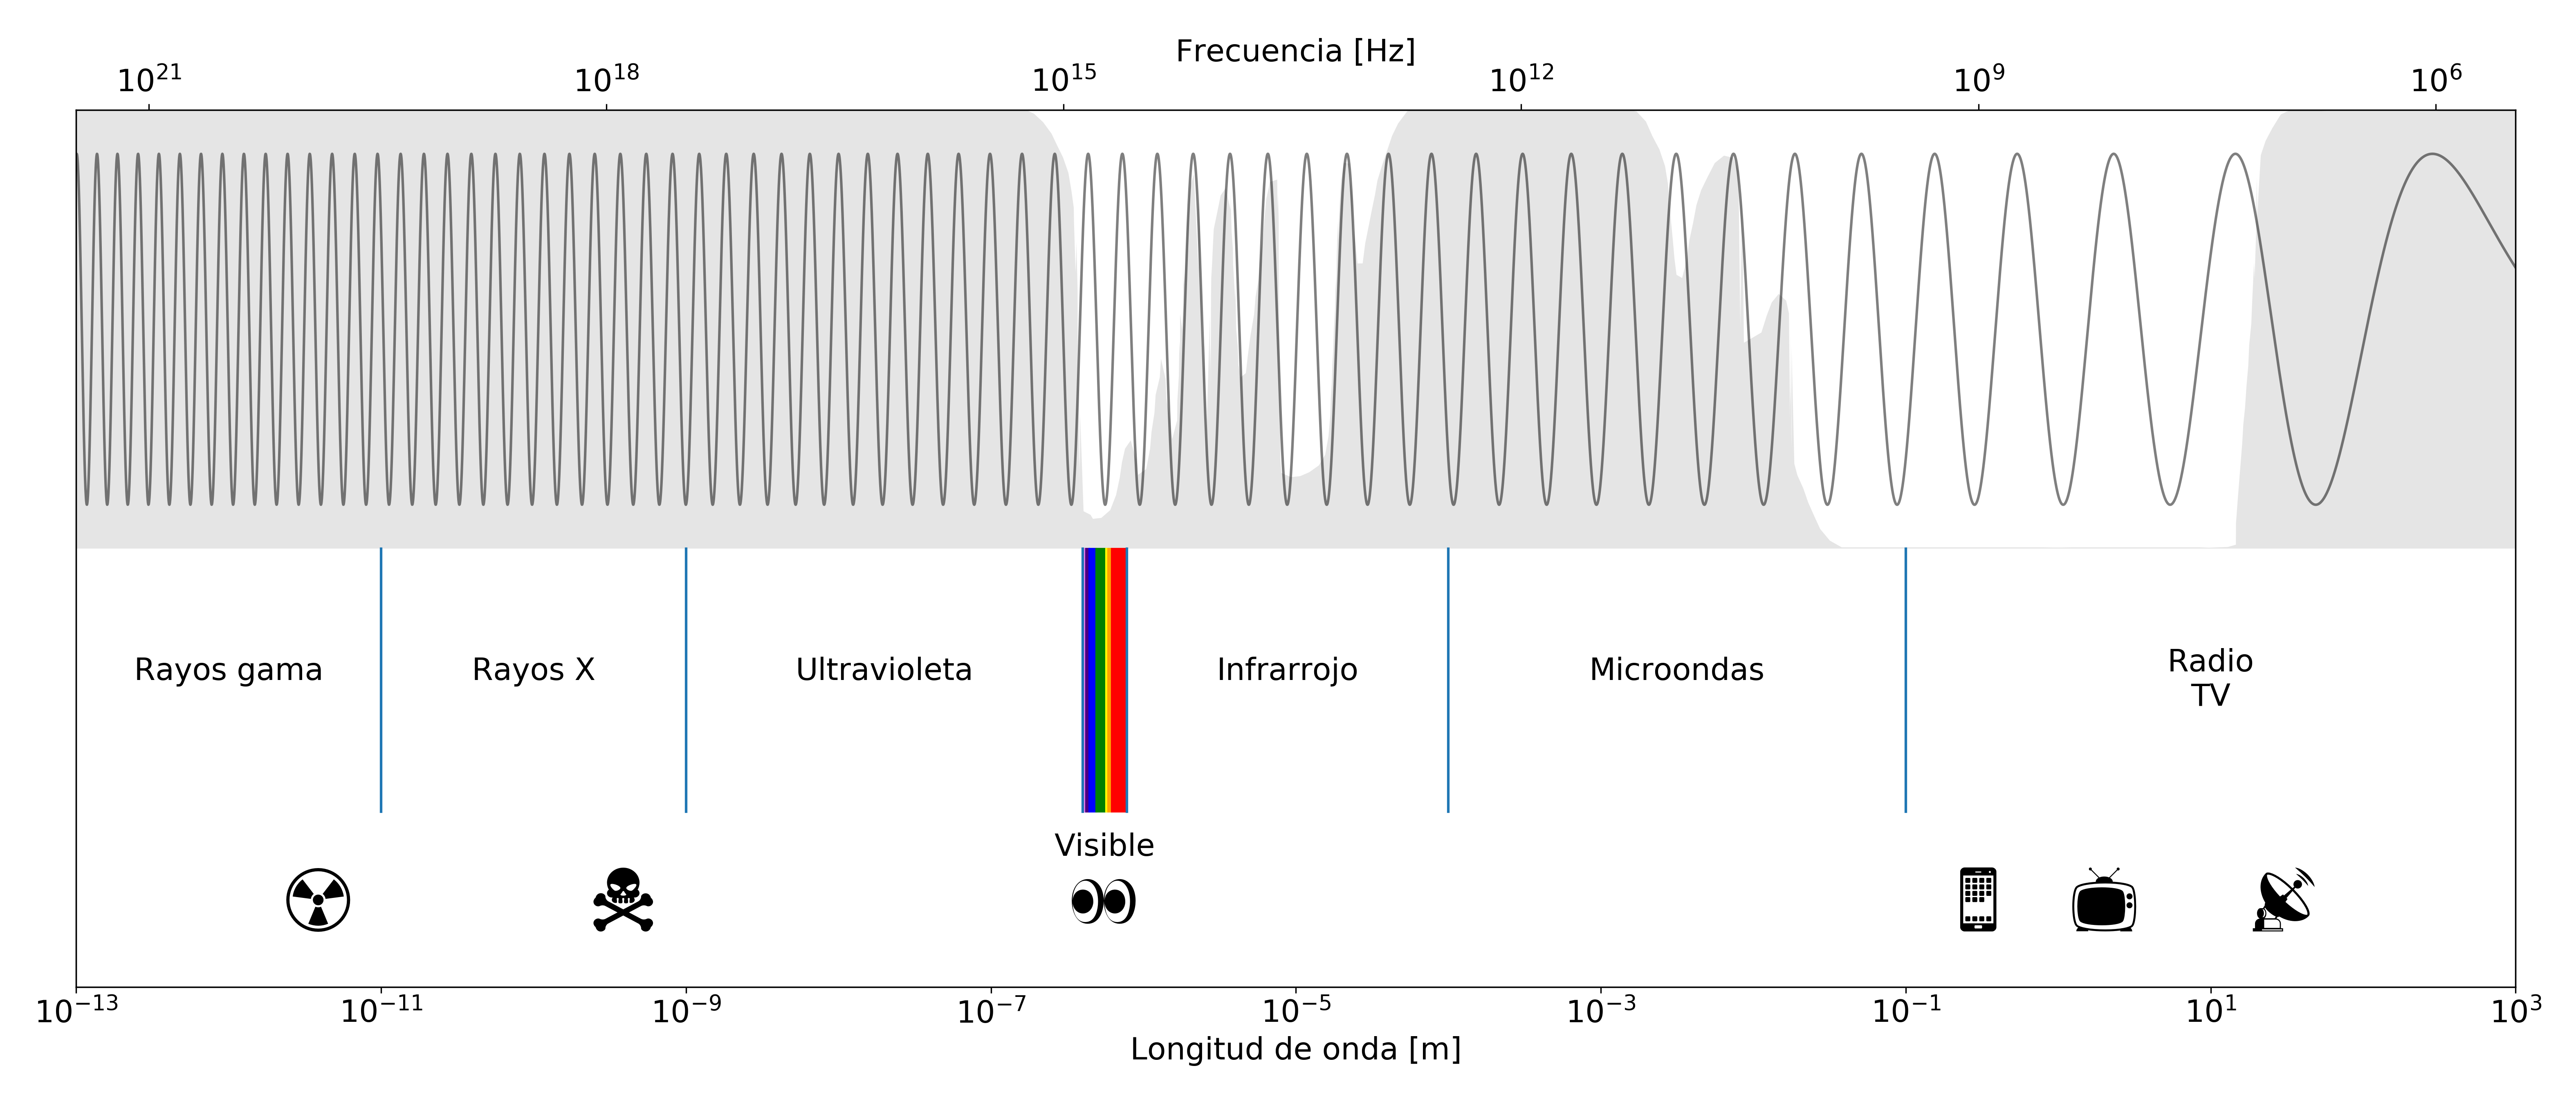
\includegraphics[width=\textwidth]{fig:espectro.png}
%    \caption{Tipos de proyecciones.}
%    \label{}
%  \end{figure}
%\end{frame}
%--- Next Frame ---%



\gracias
%--- Next Frame ---%

\section{Índices espectrales}
\subsection{Análisis espectral}

\begin{frame}{}
  \begin{figure}
    \centering
    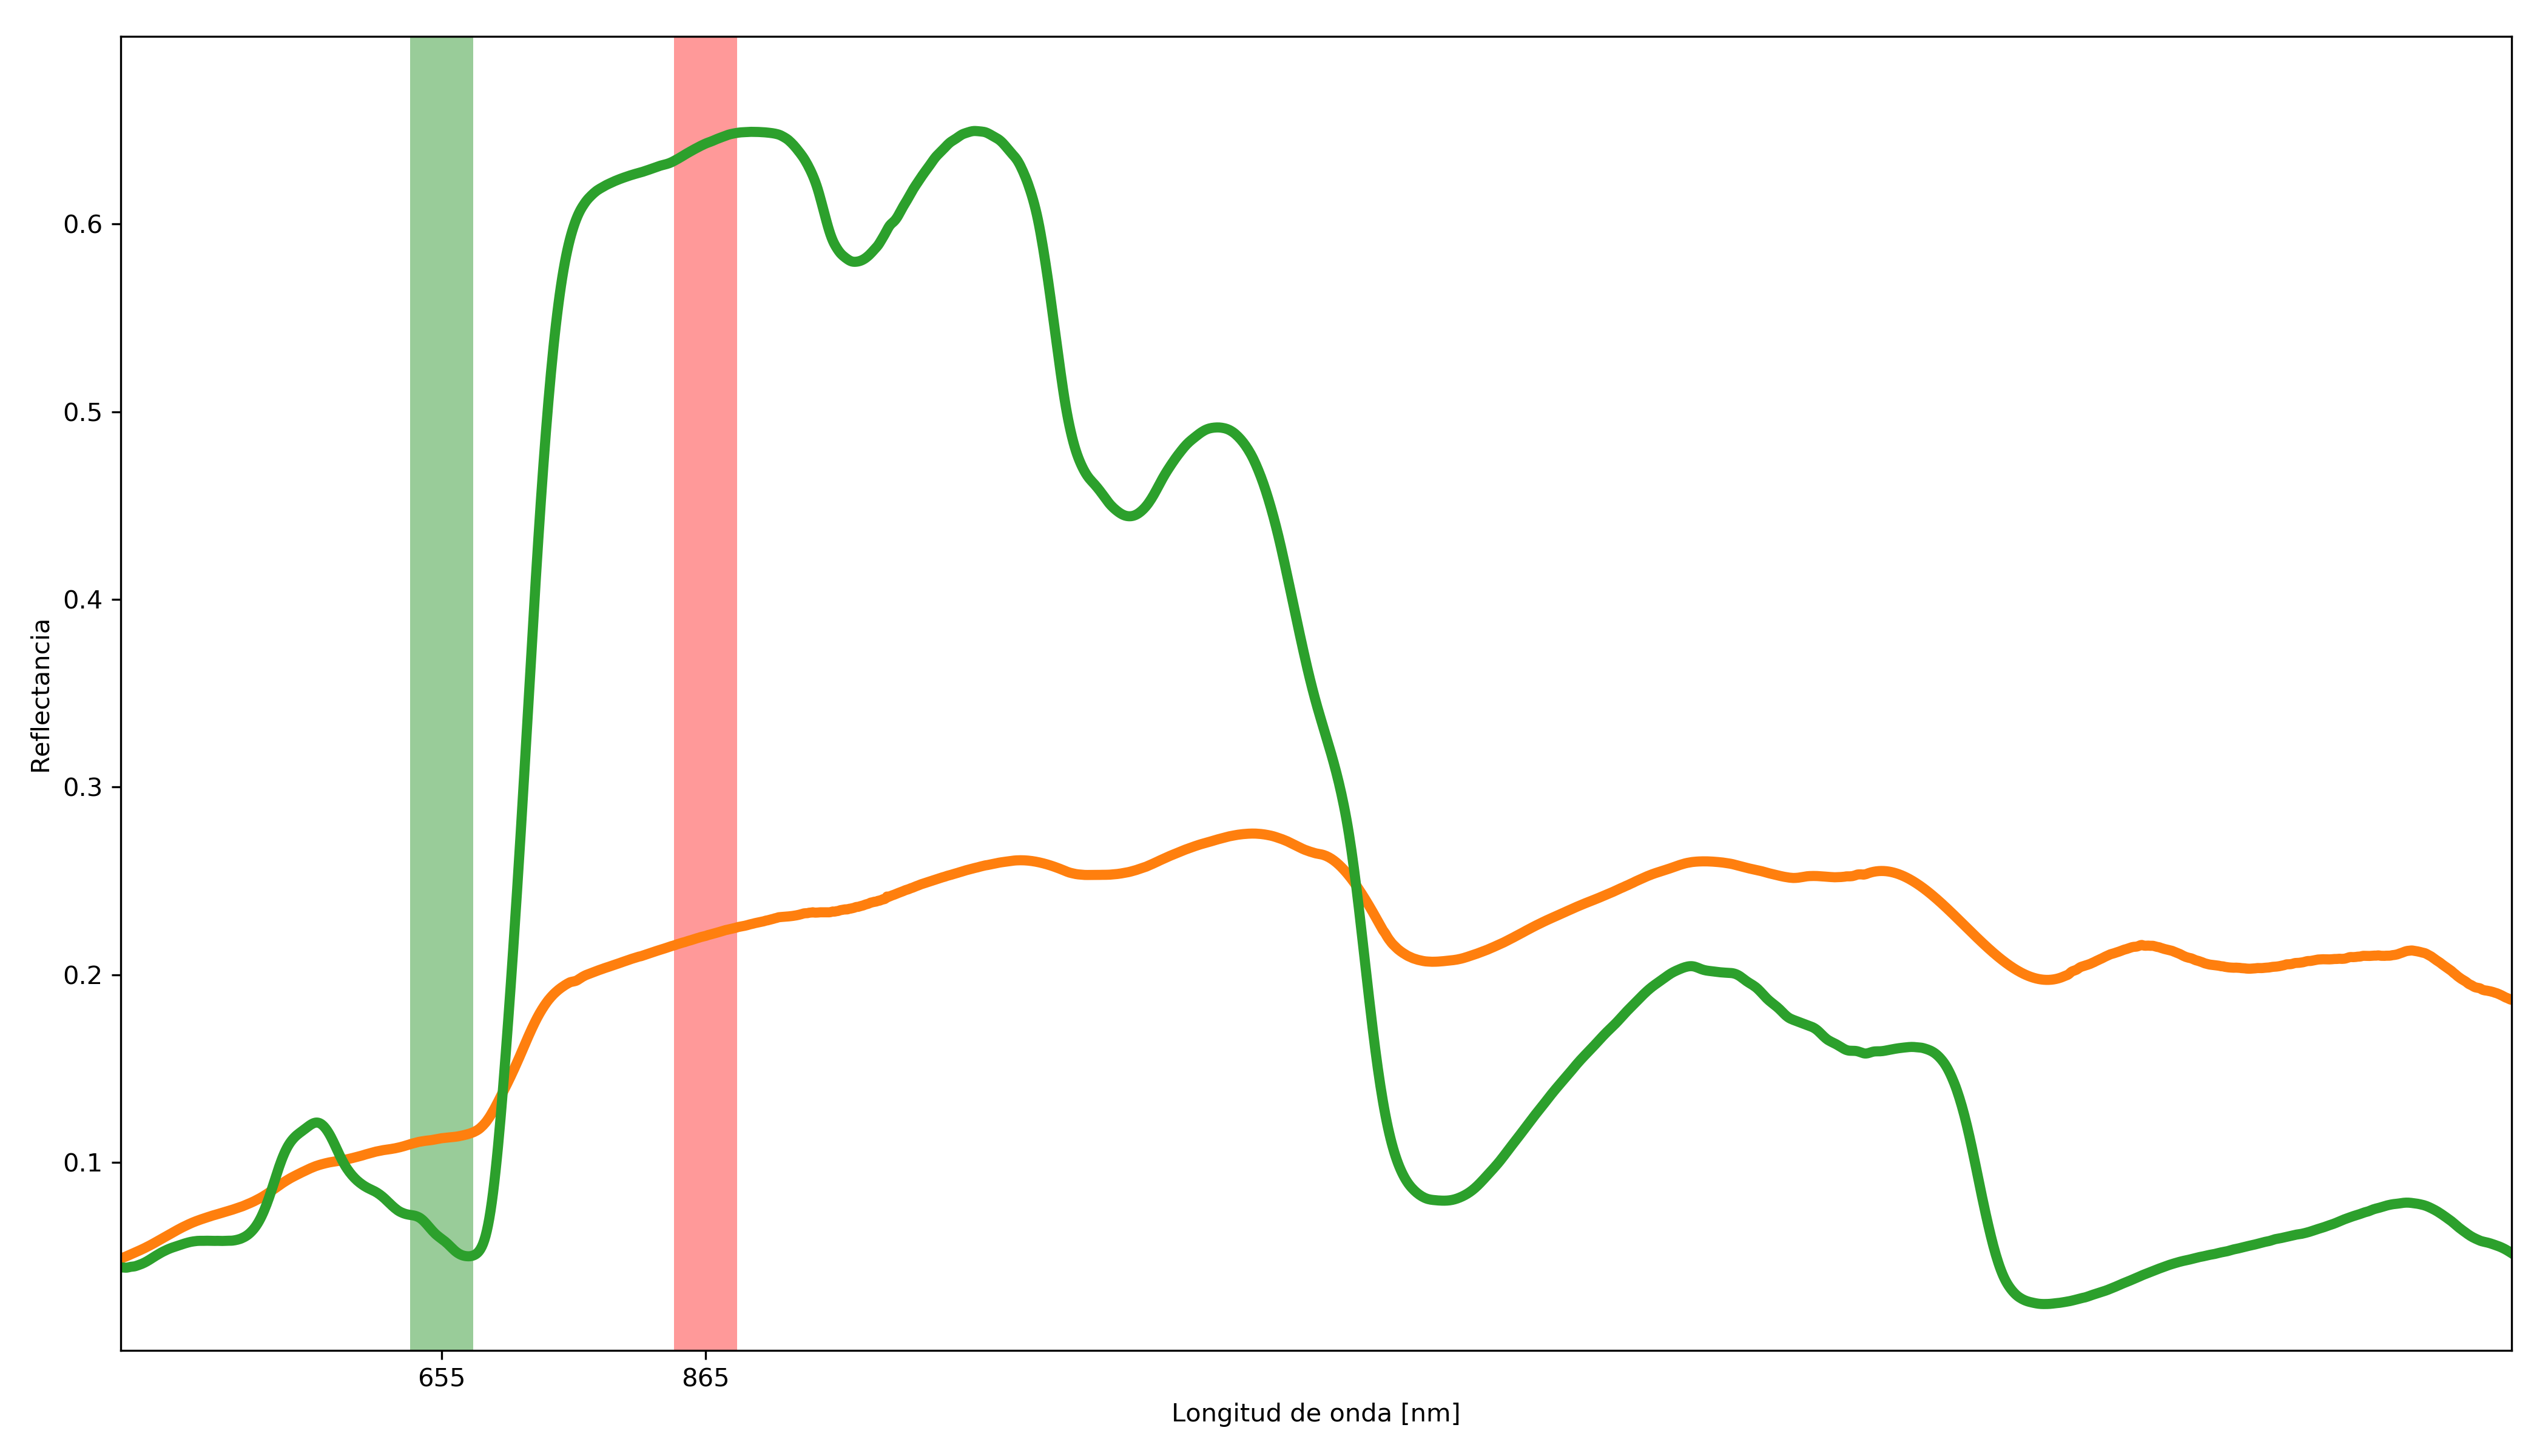
\includegraphics[width=0.8\textwidth]{fig:firmasin.png}
    \caption{Firma espectral del suelo y de la vegetación.}
    \label{}
  \end{figure}
\end{frame}
%--- Next Frame ---%
\subsection{Índices espectrales}

\begin{frame}{}
  \begin{figure}
    \centering
    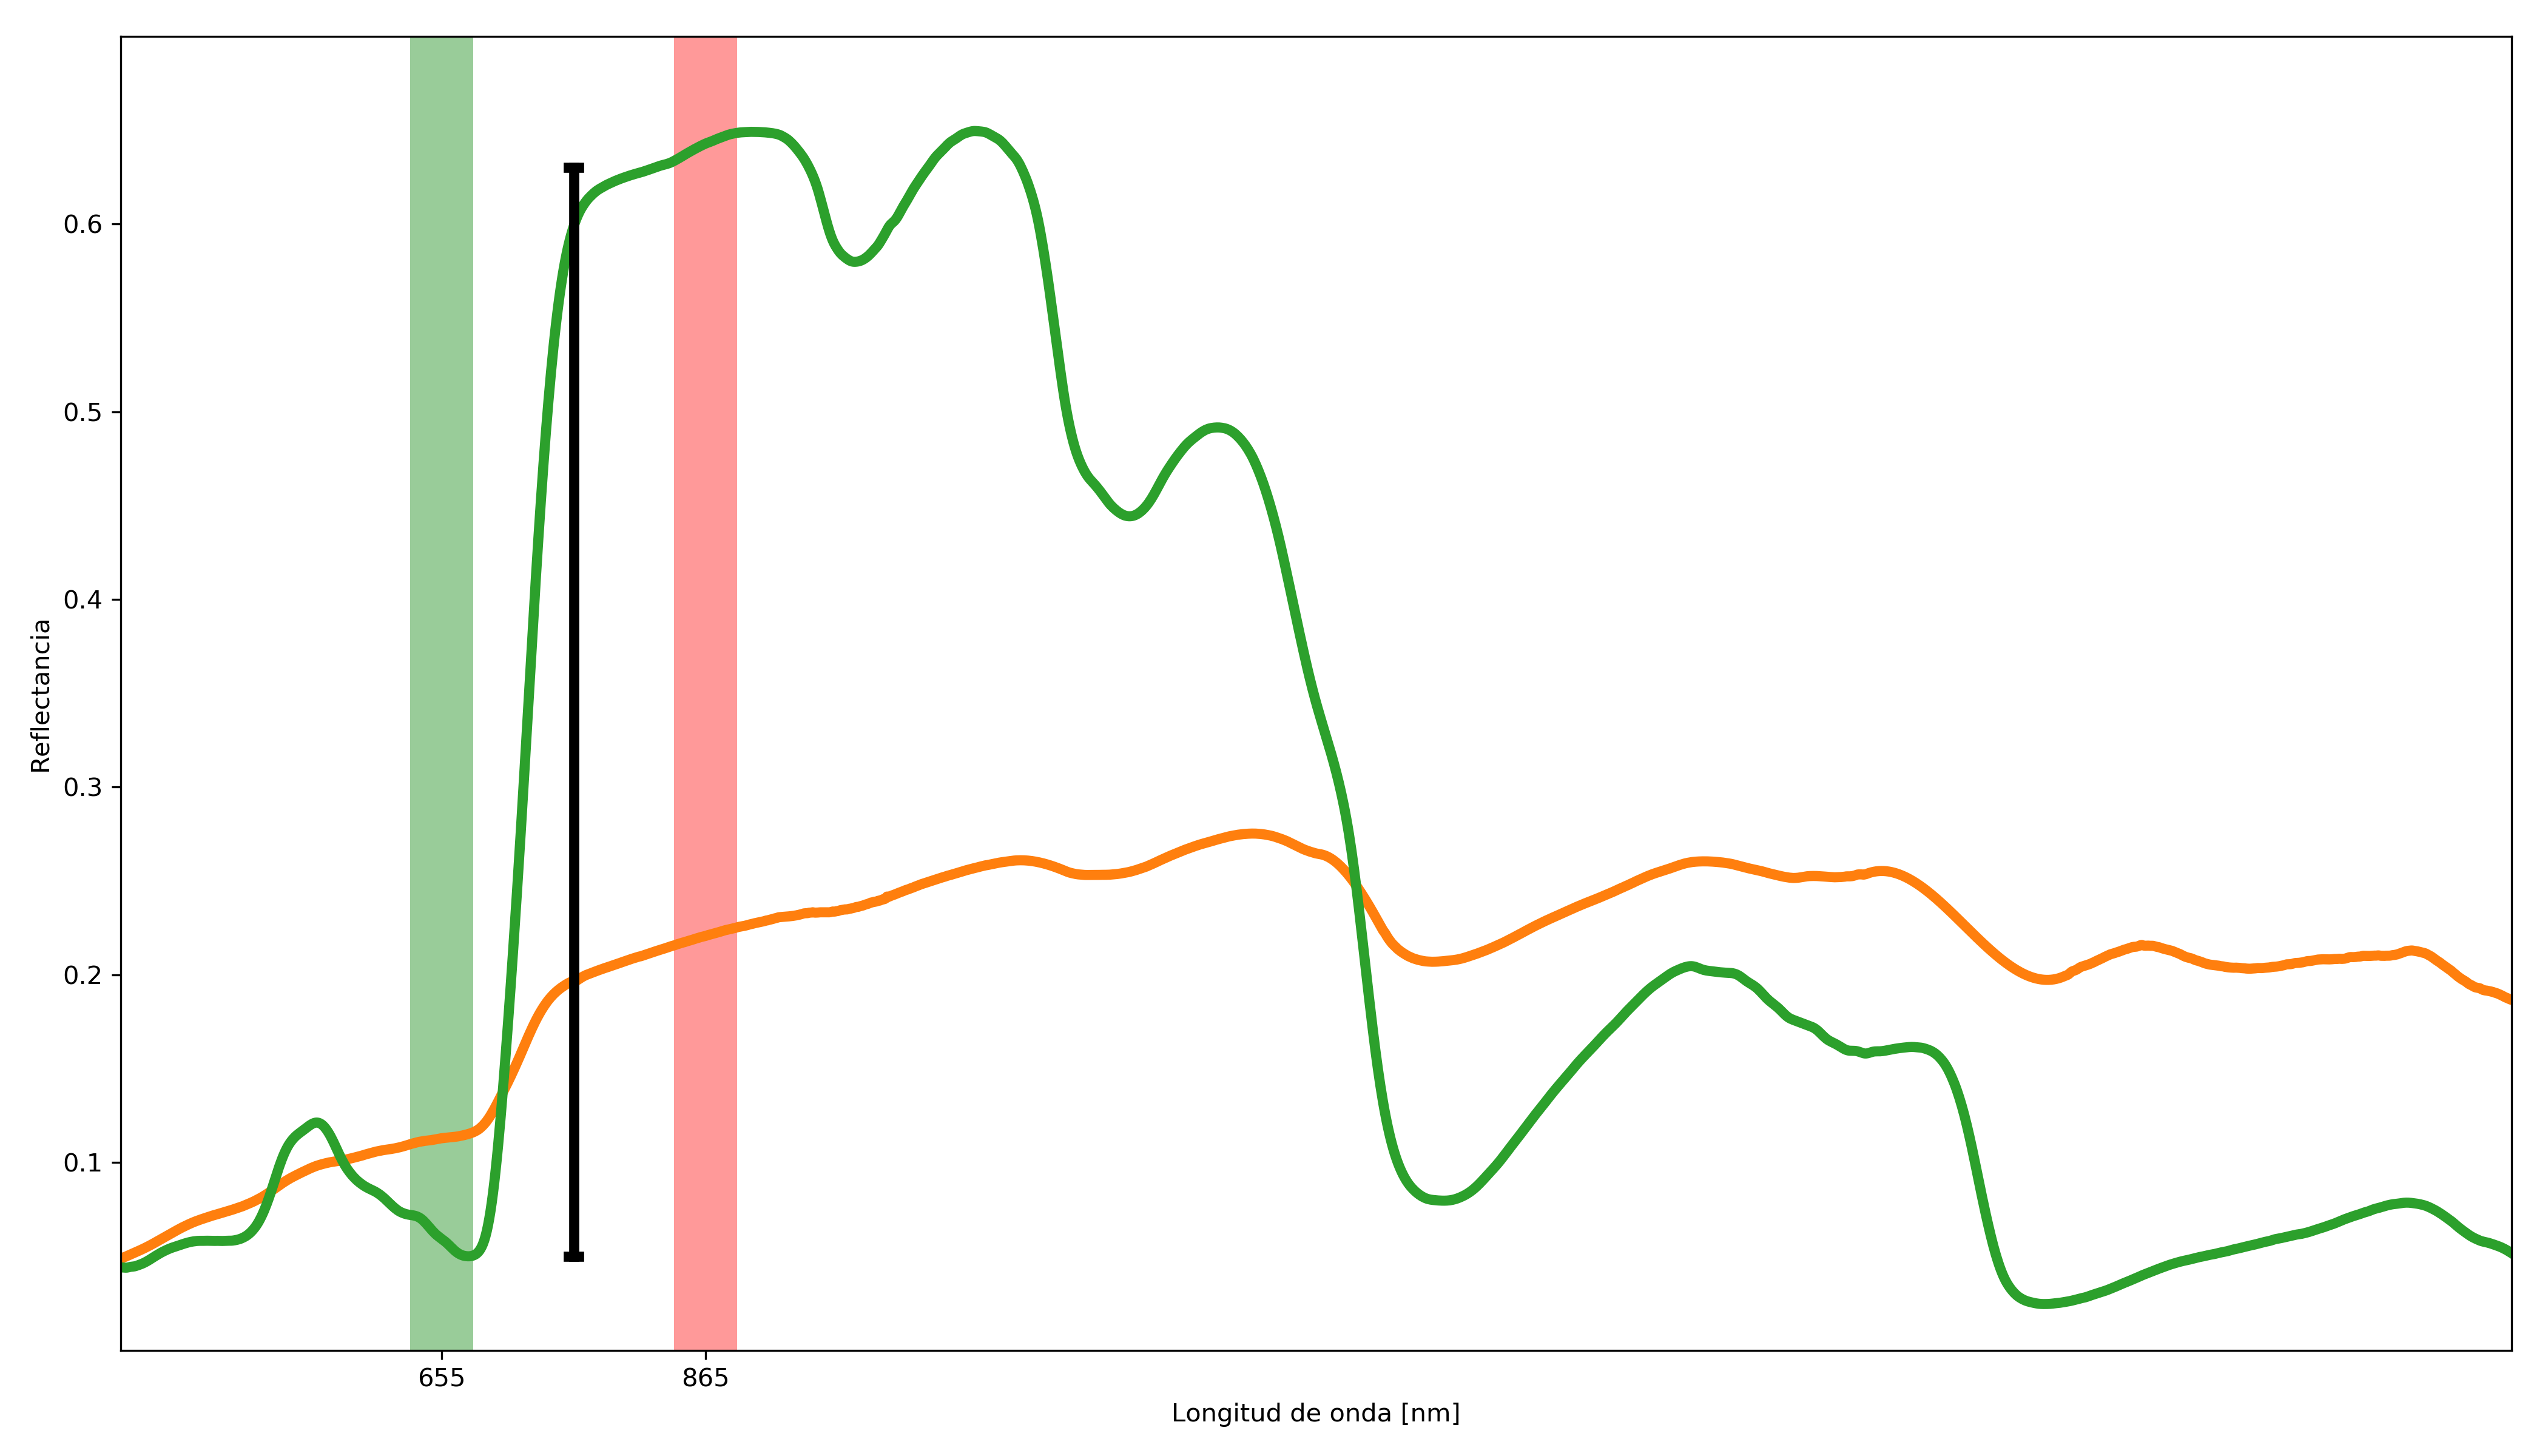
\includegraphics[width=0.8\textwidth]{fig:firmasalto.png}
    \caption{Salto $\rho_{nir}$ - $\rho_{red}$}
    \label{}
  \end{figure}
\end{frame}
%--- Next Frame ---%


\begin{frame}{}
  \begin{figure}
    \centering
    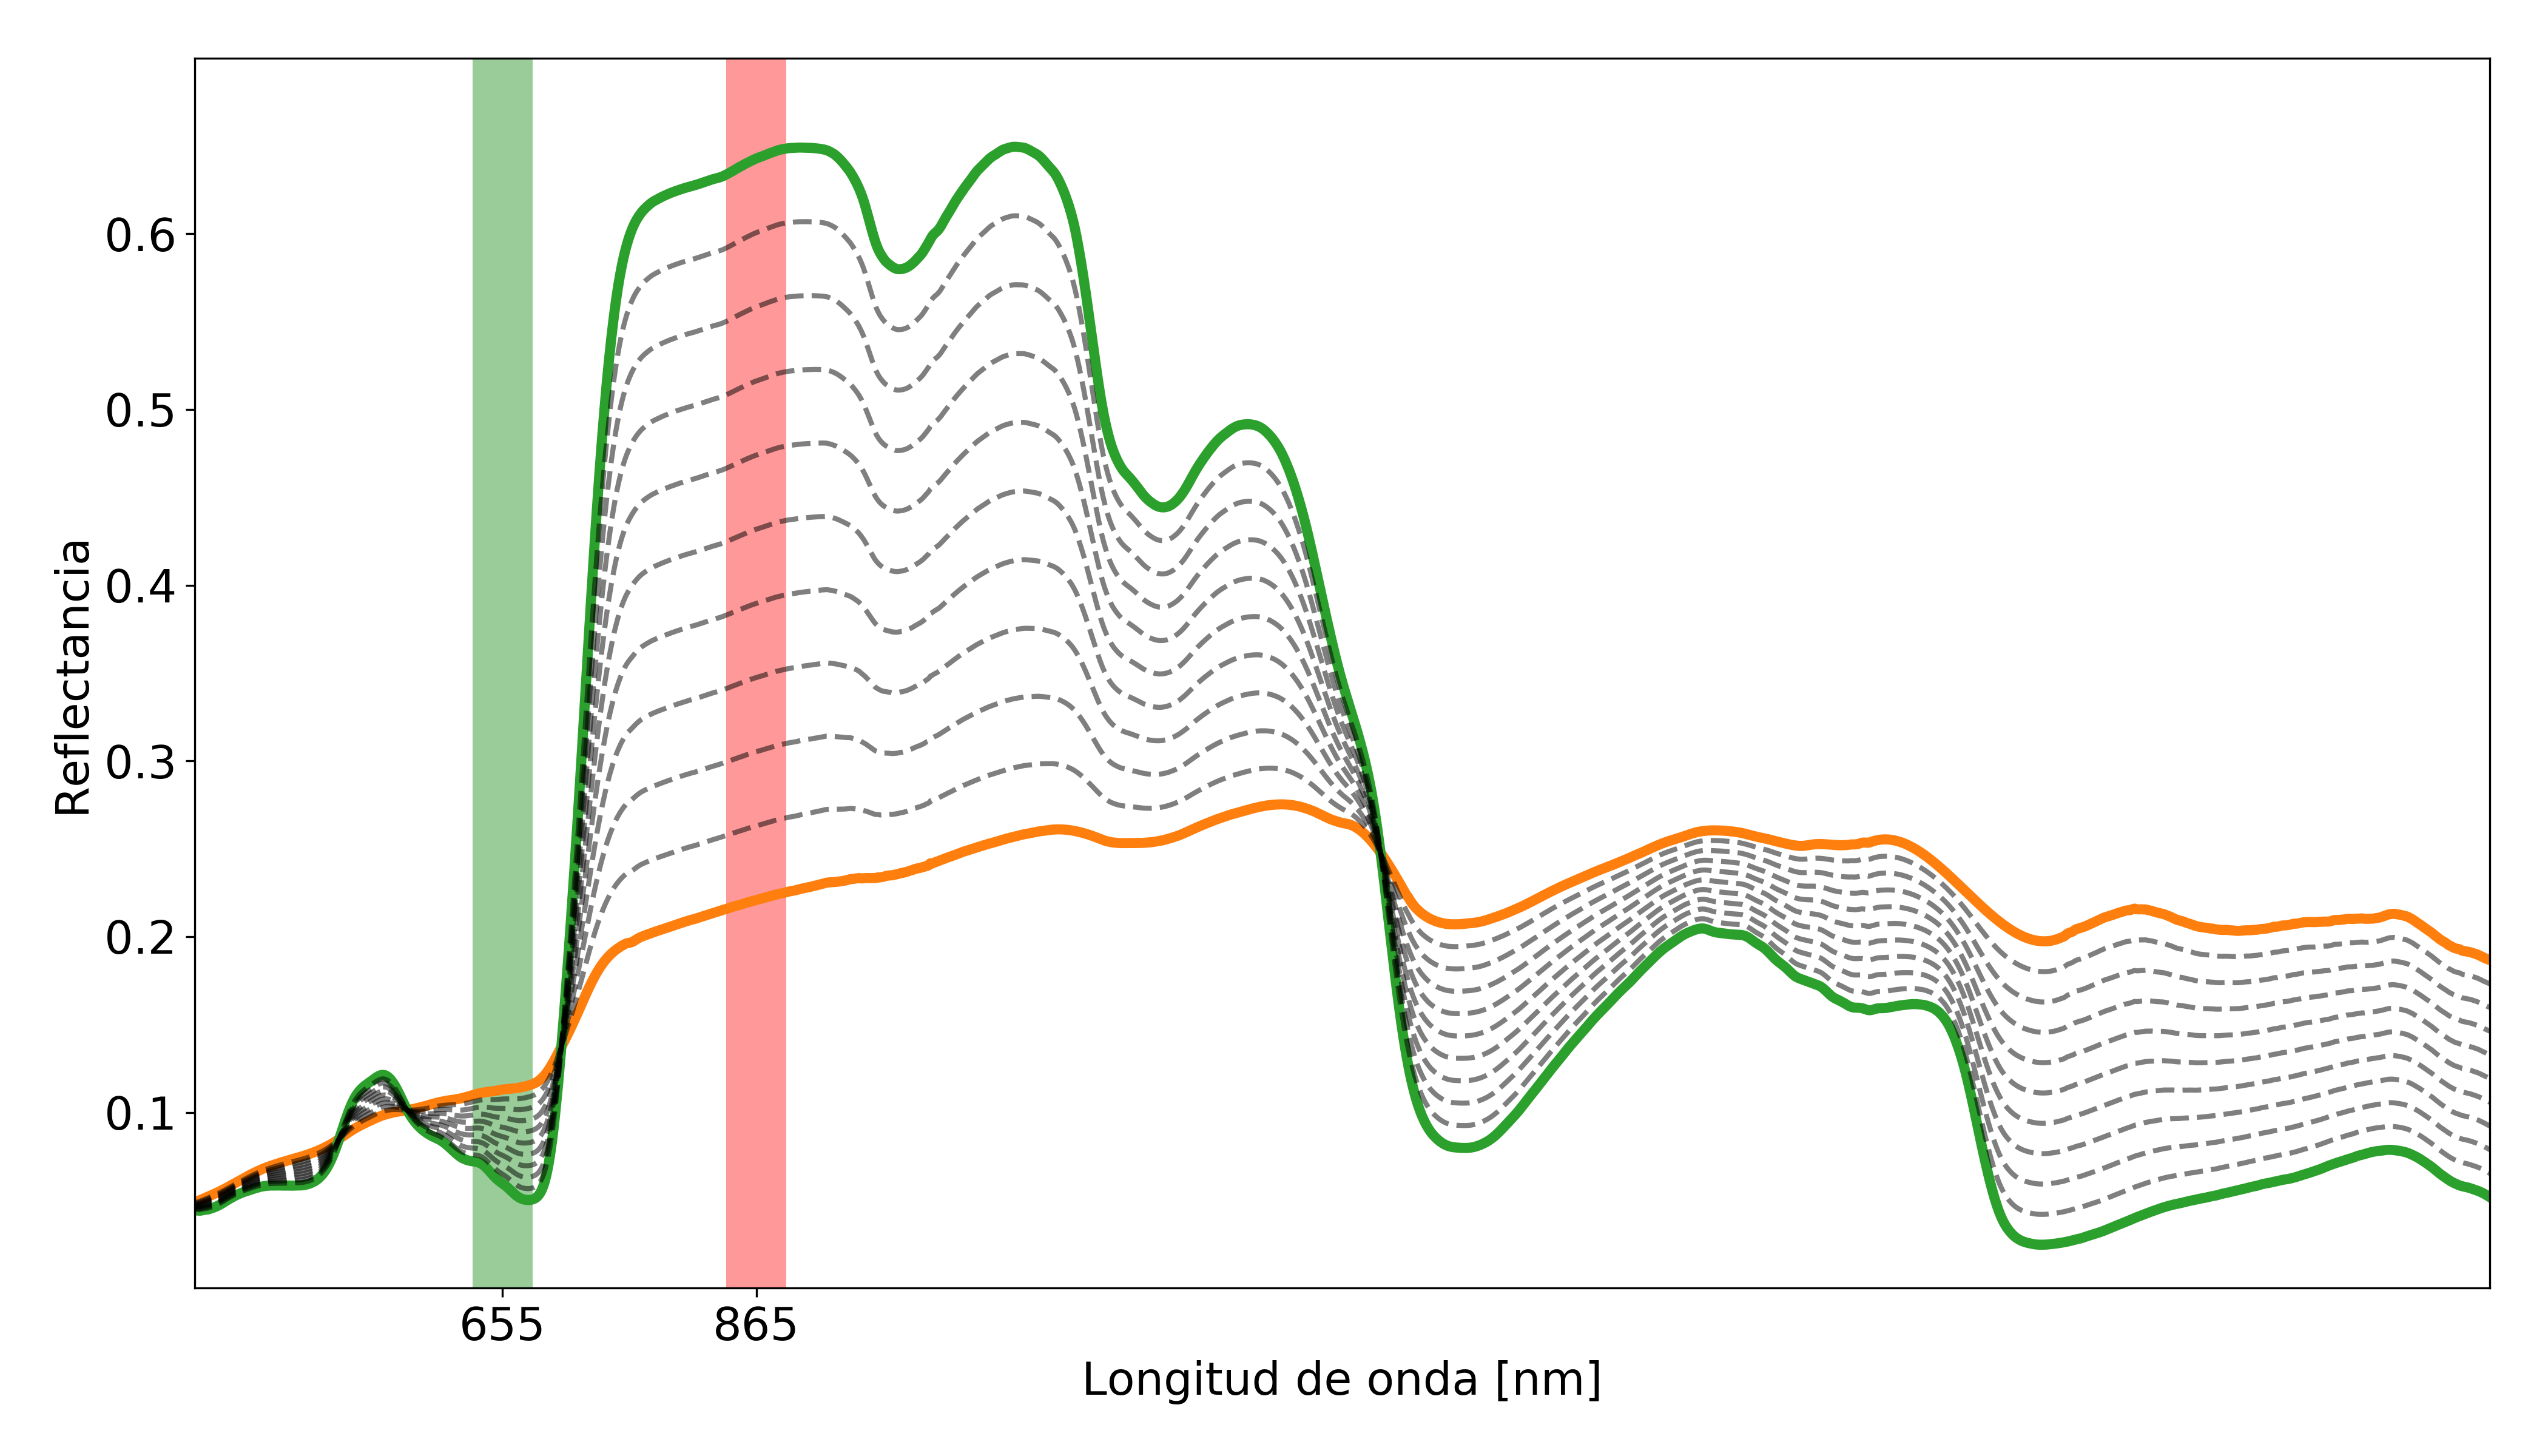
\includegraphics[width=0.8\textwidth]{fig:firmavar.png}
    \caption{Variación de la firma espectral según porcentaje de cobertura de vegetación.}
    \label{}
  \end{figure}
\end{frame}


%--- Next Frame ---%

\begin{frame}{}
  \begin{figure}
    \centering
    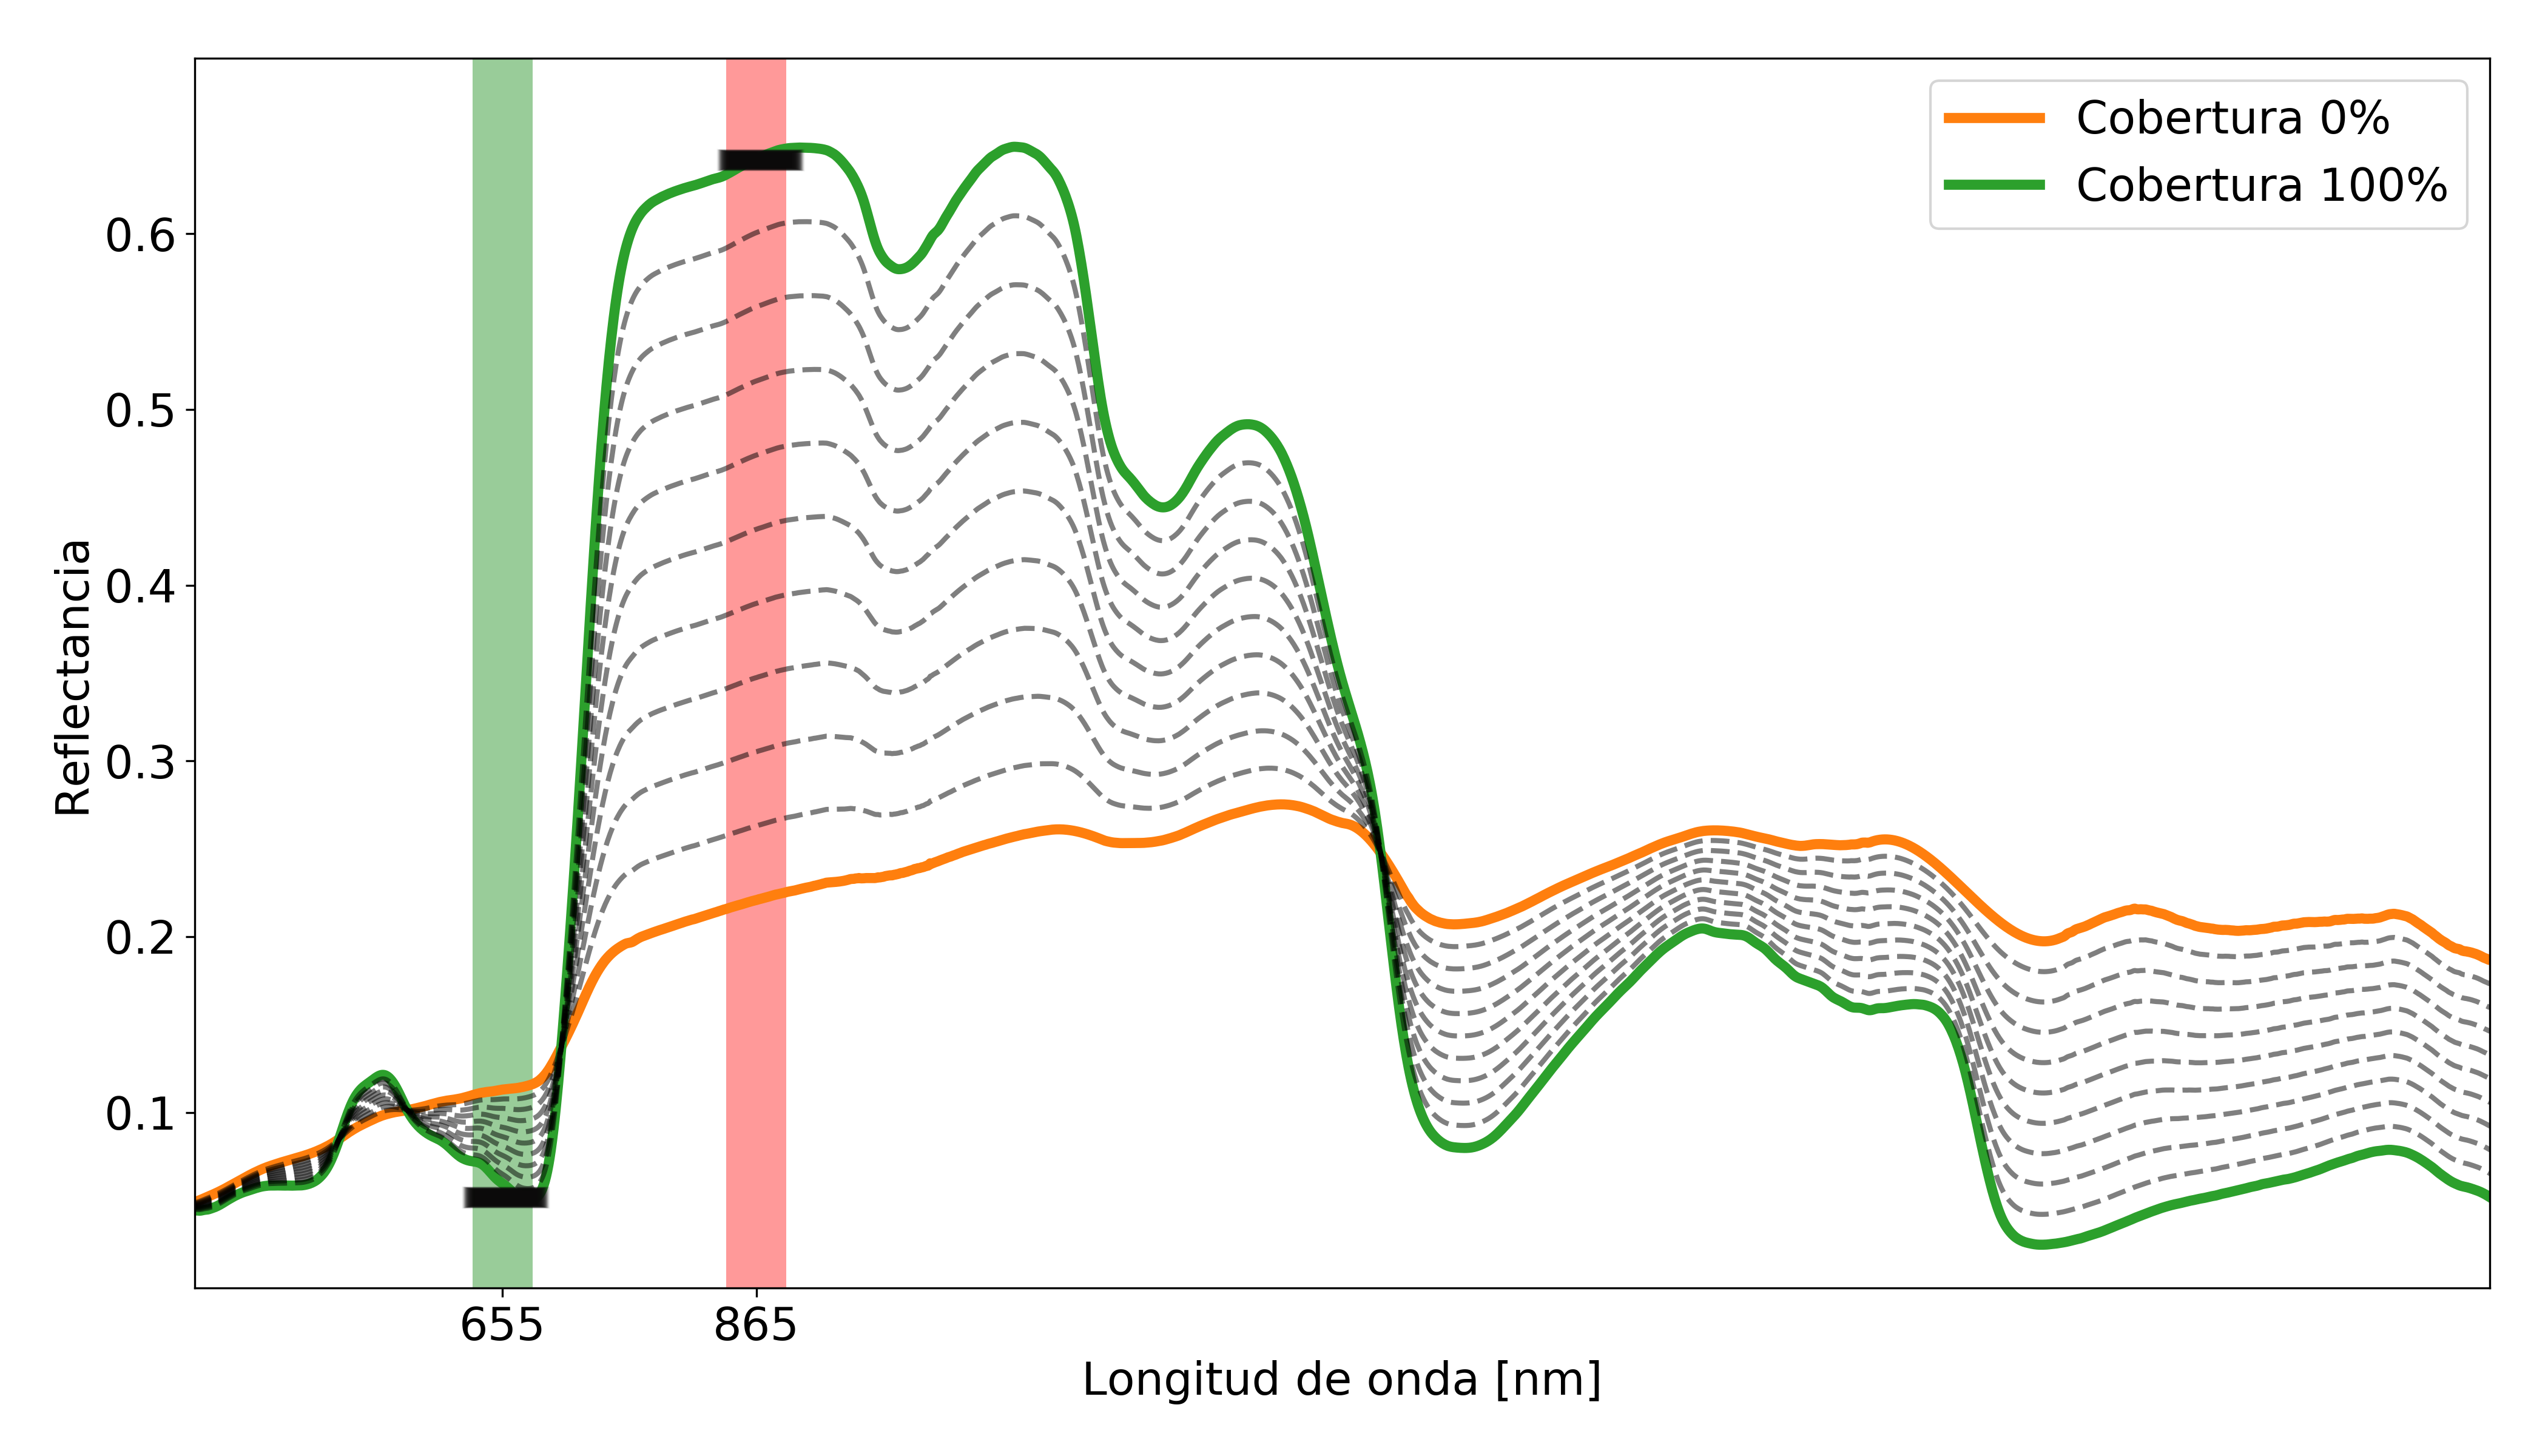
\includegraphics[width=0.8\textwidth]{fig:firmavarsr1.png}
    \caption{Variación de la firma espectral según porcentaje de cobertura de vegetación.}
    \label{}
  \end{figure}
\end{frame}

%--- Next Frame ---%
\begin{frame}
\begin{equation}
    SR = \frac{\rho_{nir}}{\rho_{nir}} = 12.6
  \end{equation}
  \end{frame}
%--- Next Frame ---%
  
\begin{frame}{}
  \begin{figure}
    \centering
    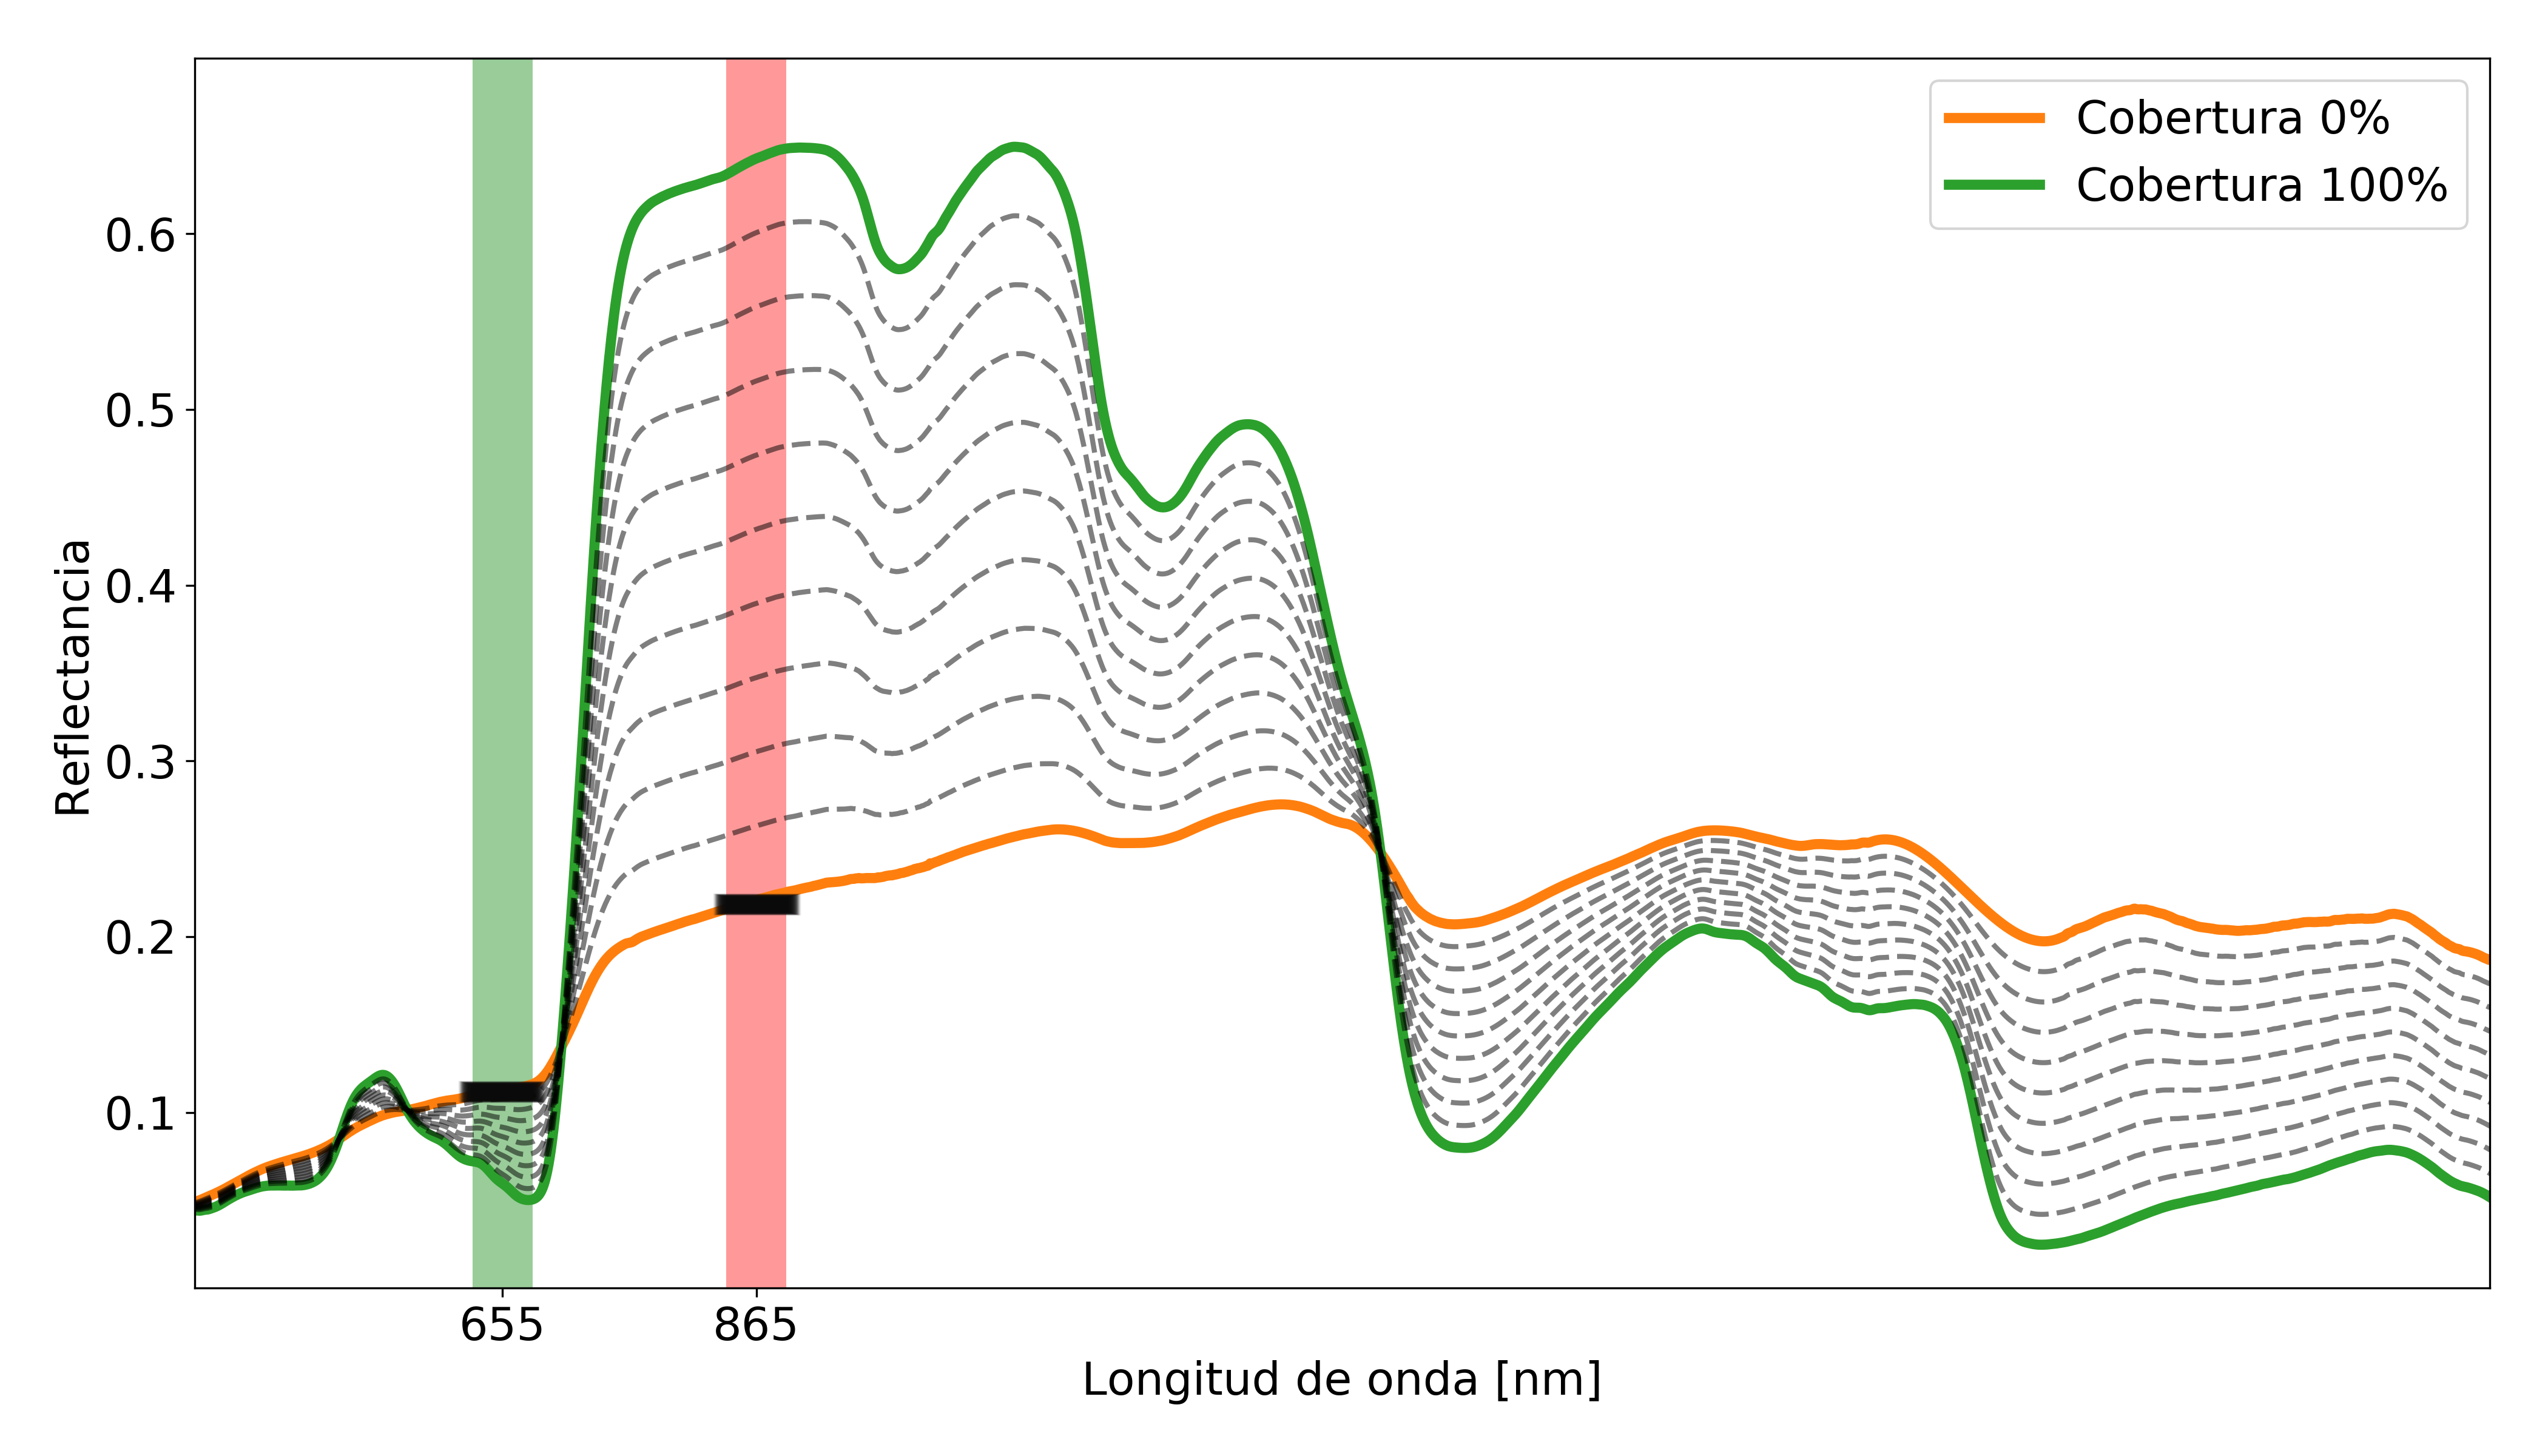
\includegraphics[width=0.8\textwidth]{fig:firmavarsr2.png}
    \caption{Variación de la firma espectral según porcentaje de cobertura de vegetación.}
    \label{}
  \end{figure}
\end{frame}

%--- Next Frame ---%
\begin{frame}
\begin{equation}
    SR = \frac{\rho_{nir}}{\rho_{nir}} = 2.1
  \end{equation}
  \end{frame}
%--- Next Frame ---%

\begin{frame}{}
\begin{block}{Normalized Difference Vegetation Index - NDVI}
  Definimos al NDVI como
  \begin{equation}
    NDVI = \frac{\rho_{nir}-\rho_{red}}{\rho_{nir}+\rho_{red}}
  \end{equation}
  con $\rho_{nir}$, $\rho_{red}$ las reflectancias en el infrarrojo cercano y el rojo, respectivamente.
\end{block}
\end{frame}

%--- Next Frame ---%

\begin{frame}{}
  \begin{figure}
    \centering
    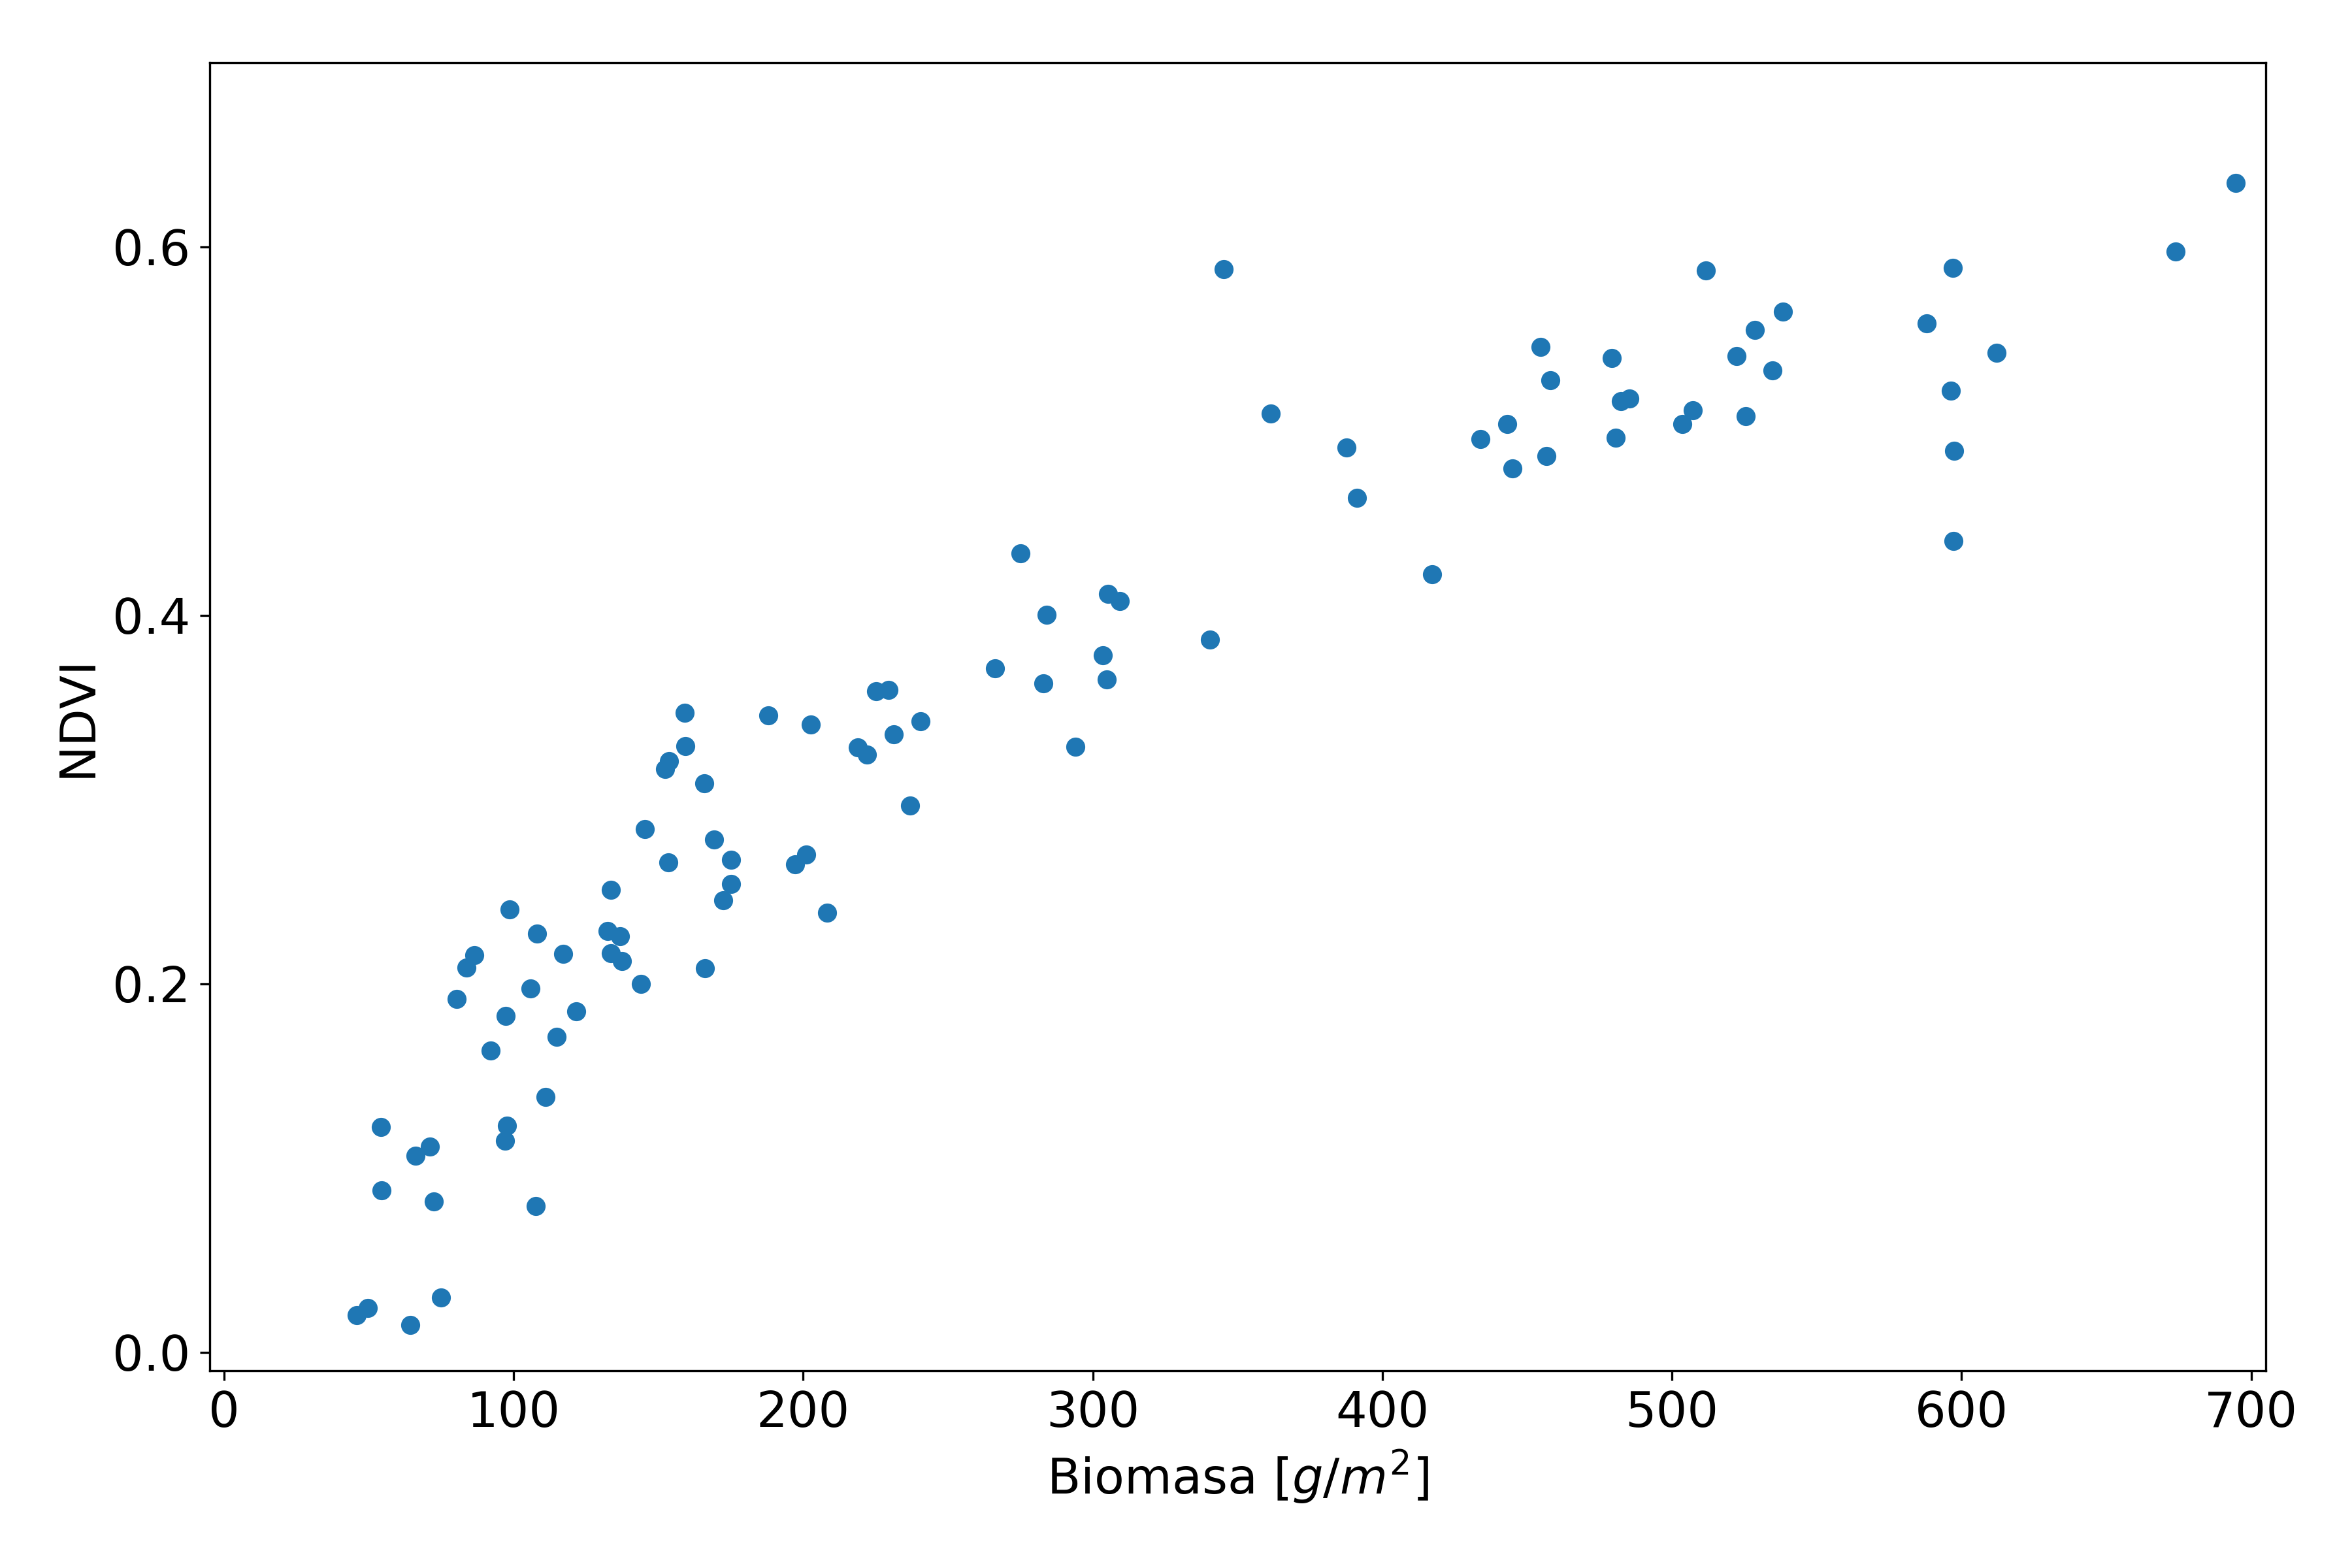
\includegraphics[width=0.7\textwidth]{fig:biomasa.png}
    \caption{Relación entre biomasa y NDVI.}
    \label{}
  \end{figure}
\end{frame}
%--- Next Frame ---%
\begin{frame}
\begin{block}{Observación}
    \begin{itemize}[<+->]
        \item La reflectancia del suelo lo puede afectar.
        \item Satura cuando el canopeo es muy denso.
    \end{itemize}
\end{block}
\end{frame}

%--- Next Frame ---%

\begin{frame}{}
    \begin{block}{Soil Adjusted Vegetation Index - SAVI}
        \begin{equation}
            SAVI = \frac{\rho_n-\rho_r}{\rho_n+\rho_r+L}(1+L)
        \end{equation}
    \end{block}\pause\
    \begin{block}{Observación}
        \begin{itemize}[<+->]
            \item Suele ajustar mejor a las variaciones de reflectancia del
                suelo.
            \item Es difícil conocer el valor de $L$ a priori. \begin{equation}
        L=0.5
    \end{equation}
        \end{itemize}
    \end{block}
\end{frame}

\begin{frame}{}
    \begin{block}{Enhanced Vegetation Index - EVI}
        \begin{equation}
            EVI = G\frac{\rho_n - \rho_r}{\rho_n+C_1\rho_r-C_2\rho_b+L}(1+L)
        \end{equation}
    \end{block}
    donde
    \begin{itemize}
        \item $G  \sim 2.5$
        \item $C1 \sim 6.0$
        \item $C2 \sim 7.5$
        \item $L  \sim 1.0$
    \end{itemize}
\end{frame}

\gracias
%--- Next Frame ---%

\section{Misión SAOCOM y aplicaciones}
\subsection{Misiones SAOCOM}
\begin{frame}{\secname : \subsecname}
  \begin{figure}
    \centering
    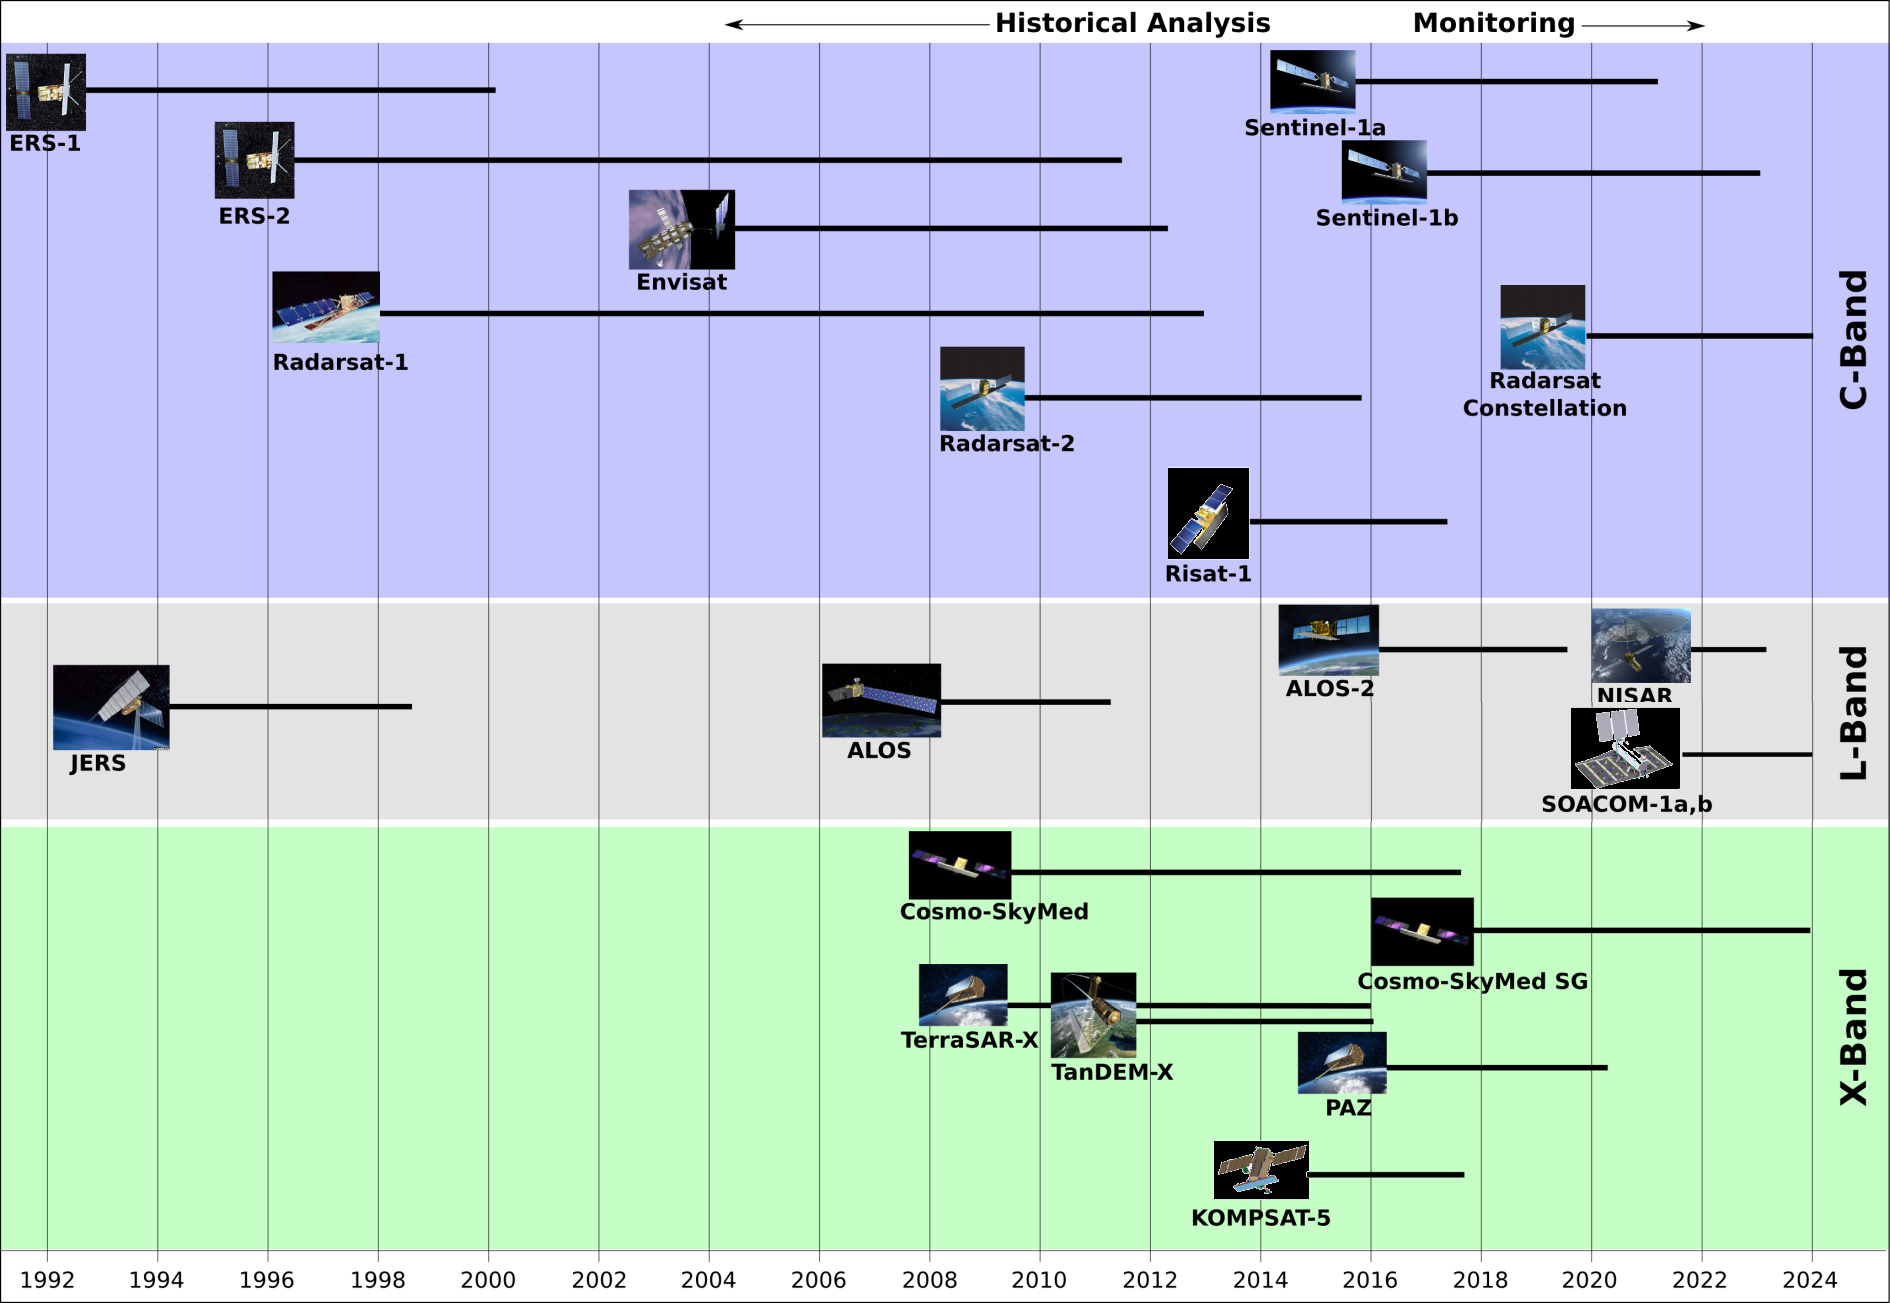
\includegraphics[width=0.7\textwidth]{fig:misiones}
    \caption{Misiones satelitales historicas y actuales.}
    \label{}
  \end{figure}
\end{frame}
%--- Next Frame ---%

\begin{frame}{\secname : \subsecname}
  \begin{figure}
    \centering
    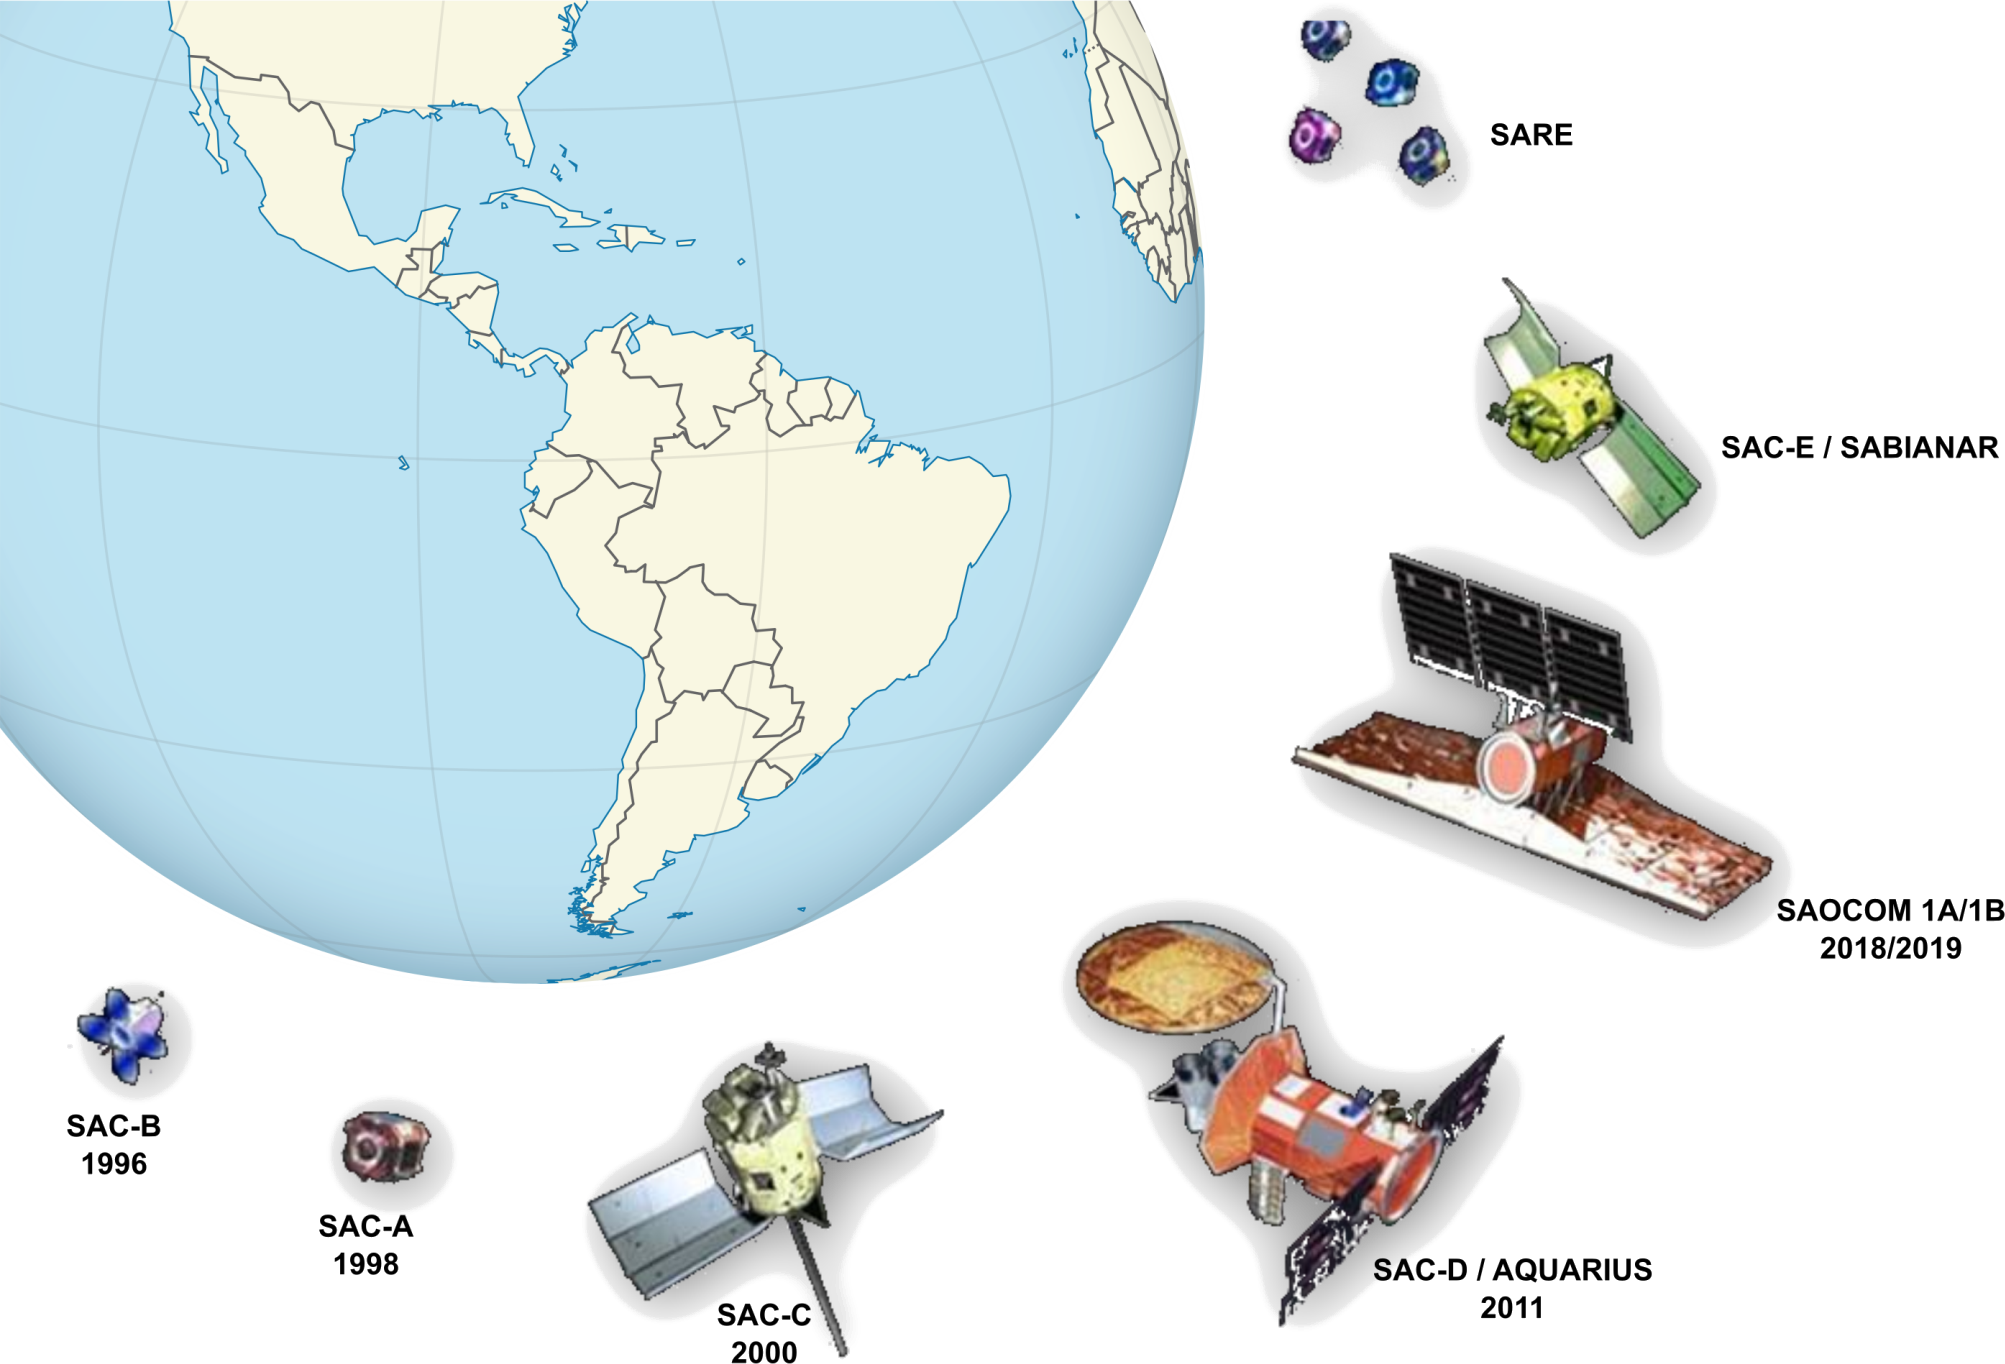
\includegraphics[width=0.65\textwidth]{fig:plan}
    \caption{Satelites del plan espacial nacional.}
    \label{}
  \end{figure}
\end{frame}
%--- Next Frame ---%

\begin{frame}{\secname : \subsecname}
  \begin{columns}
    \begin{column}{0.6\textwidth}
     \begin{block}{Mision SAOCOM}
\begin{itemize}
  \item Dos satélites idénticos
  \item L-Band SAR (1275 Mhz)
  \item Cobertura Global
  \item Mirada a derecha
  \begin{itemize}
    \item Adquisiciones continuas de 10 minutos en visibilidad de una estación
    \item 15 minutos por órbita en promedio
    \item 20 minutos de adquisiciones no continuas en una órbita
  \end{itemize}
  \item Mirada a izquierda
  \begin{itemize}
    \item Hasta 5 minutos
  \end{itemize}
  \item Antena activa de 10m x 3.5m con 140 MTR
\end{itemize}
     \end{block}
    \end{column}
    \begin{column}{0.4\textwidth}  %%<--- here
      \begin{figure}
        \centering
        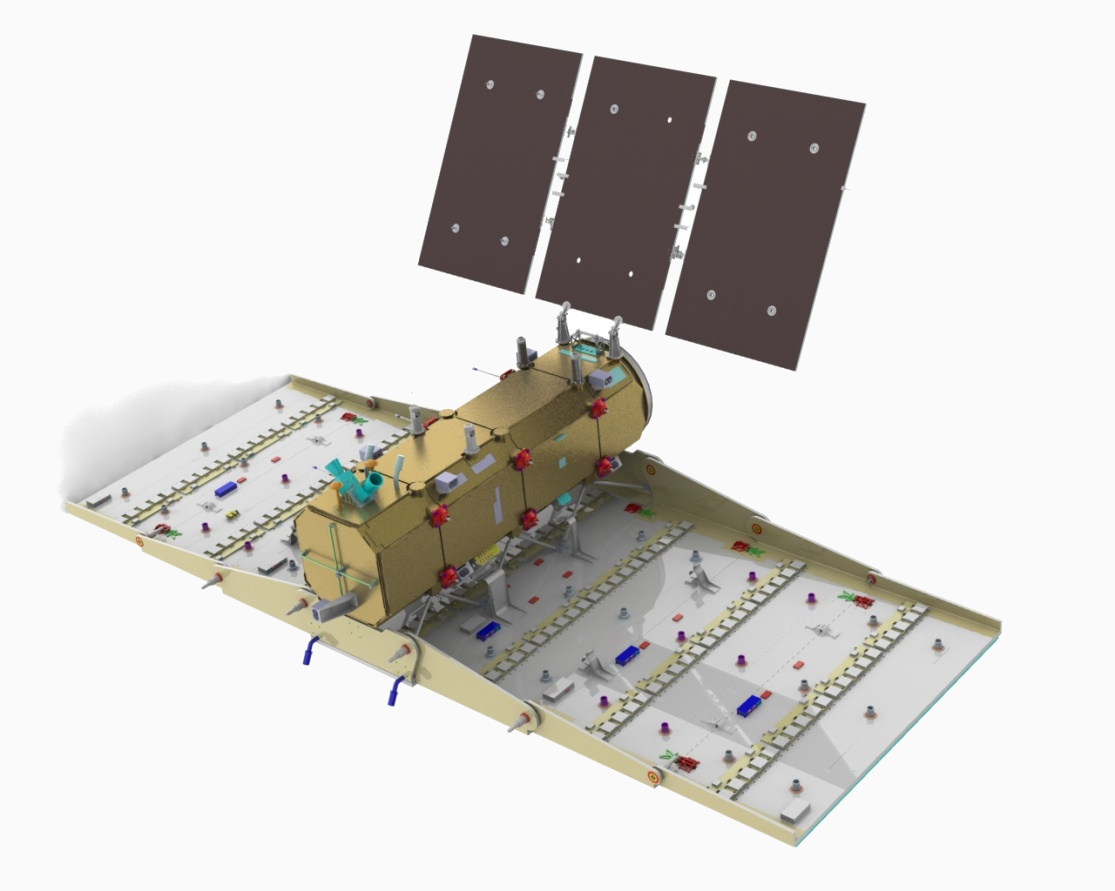
\includegraphics[width=1.1\textwidth]{fig:saocom.jpg}
        \caption*{}
        \label{}
      \end{figure}
    \end{column}
    \end{columns}

\end{frame}
%--- Next Frame ---%

\begin{frame}{\secname : \subsecname}
\begin{itemize}
  \item Órbita polar, heliosincrónica (inclinación 97.89) a 620 km de altura
  \item Cada satélite esta desfasado 180 grados
  \item Hora local de pasada por el Ecuador en forma ascendente : 06:12 am
  \item Duración de la orbita 97,2 minutos
  \item Tiempo de revisita: 16 días (1 satélite) / 8 días (constelación)
  \item Orbitas por ciclo: 237
  \item 23 ciclos por año
\end{itemize}
\end{frame}
%--- Next Frame ---%

\subsection{Aplicaciones SAR}

\begin{frame}{\secname : \subsecname}
  \begin{figure}
    \centering
    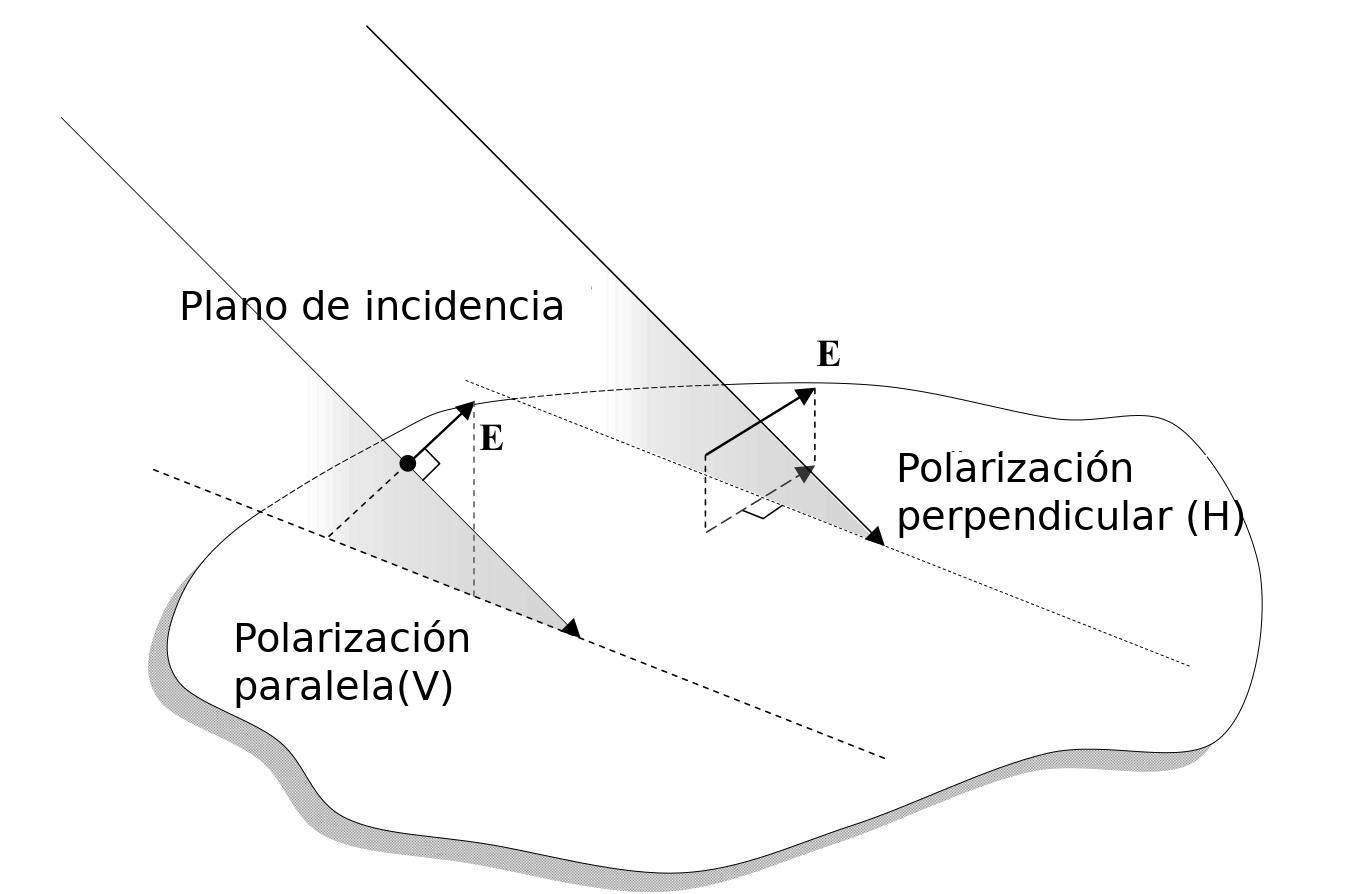
\includegraphics[width=0.6\textwidth]{fig:polarizacion.png}
    \caption{Cálculo de la humedad del suelo.}
    \label{}
  \end{figure}
\end{frame}
%--- Next Frame ---%

\begin{frame}{\secname : \subsecname}
  \begin{figure}
    \centering
    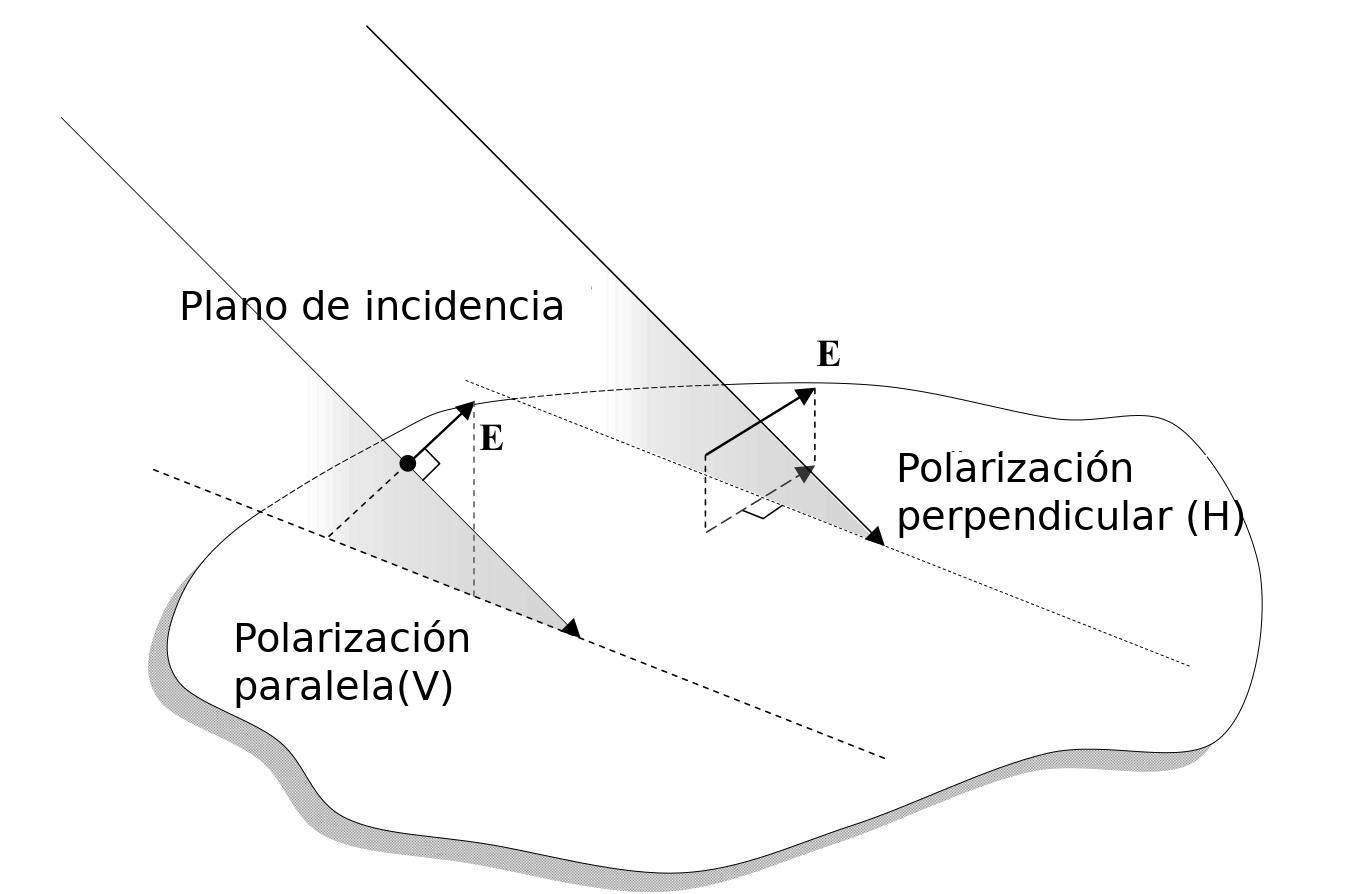
\includegraphics[width=0.6\textwidth]{fig:polarizacion.png}
    \caption{Cálculo de la rugosidad del suelo.}
    \label{}
  \end{figure}
\end{frame}
%--- Next Frame ---%

\begin{frame}{\secname : \subsecname}
  \begin{figure}
    \centering
    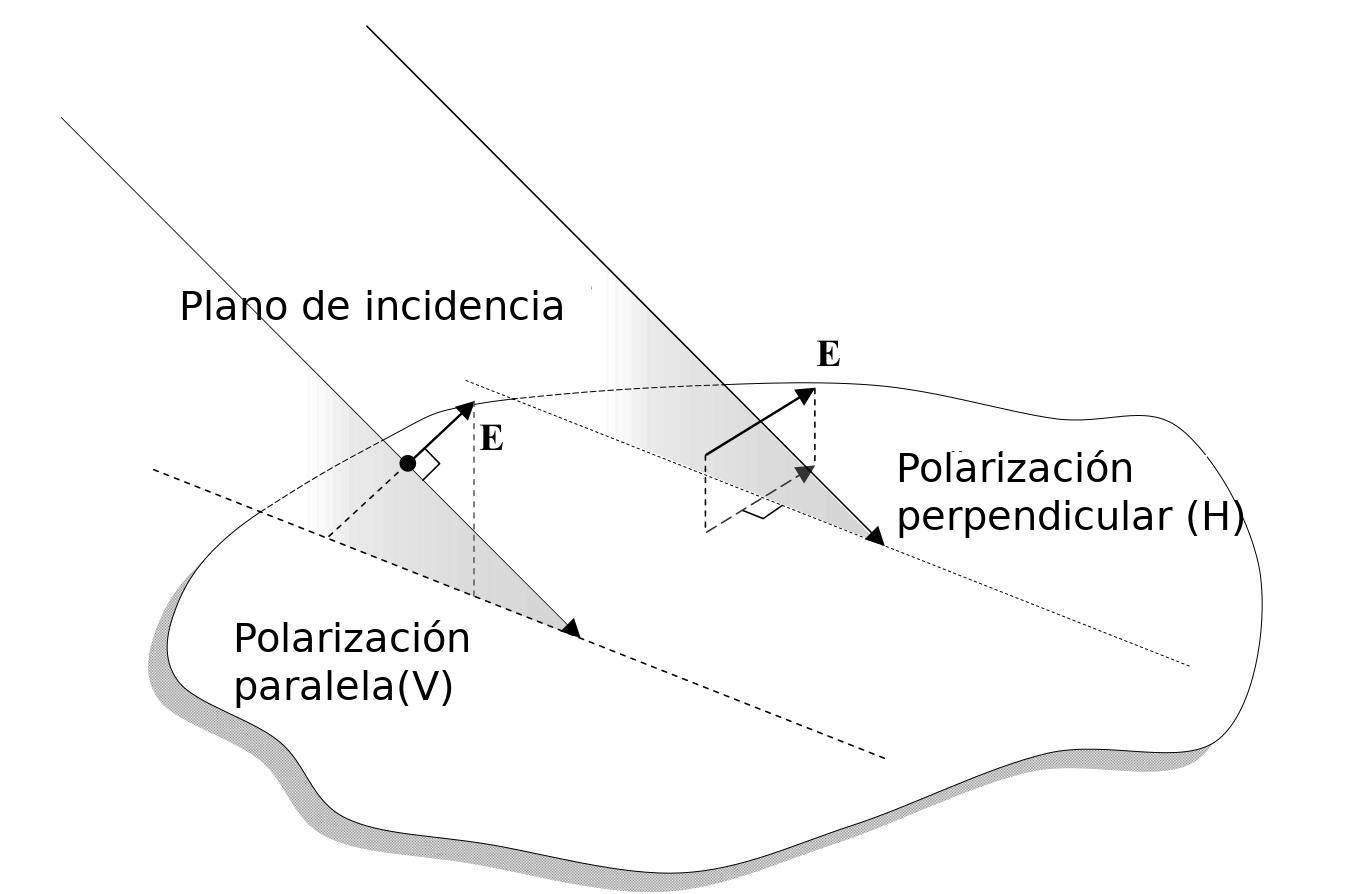
\includegraphics[width=0.6\textwidth]{fig:polarizacion.png}
    \caption{Detección de cuerpos de água.}
    \label{}
  \end{figure}
\end{frame}
%--- Next Frame ---%

\begin{frame}{\secname : \subsecname}
  \begin{figure}
    \centering
    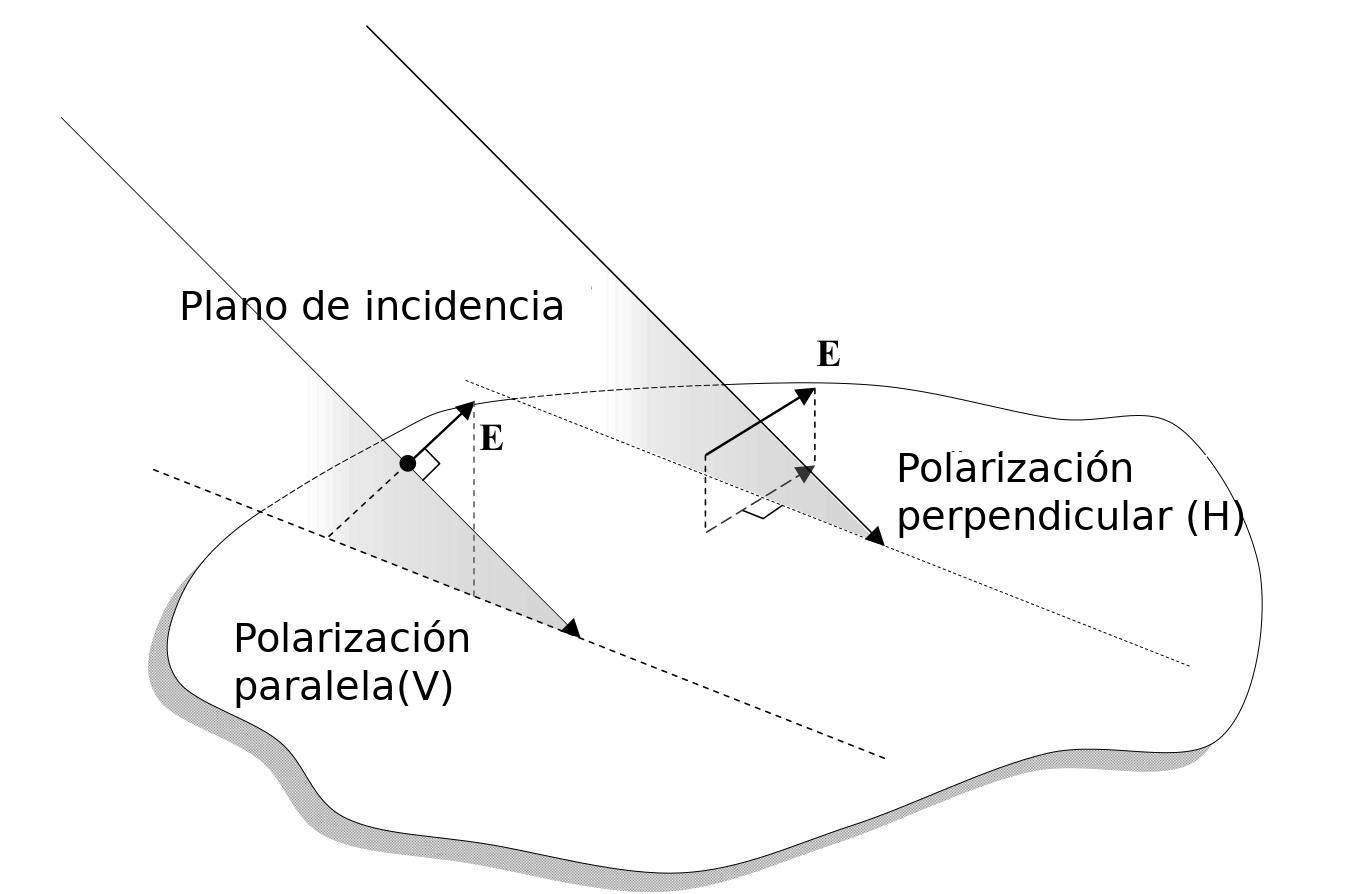
\includegraphics[width=0.6\textwidth]{fig:polarizacion.png}
    \caption{Clasificación de cultivos.}
    \label{}
  \end{figure}
\end{frame}
%--- Next Frame ---%

\begin{frame}{\secname : \subsecname}
  \begin{figure}
    \centering
    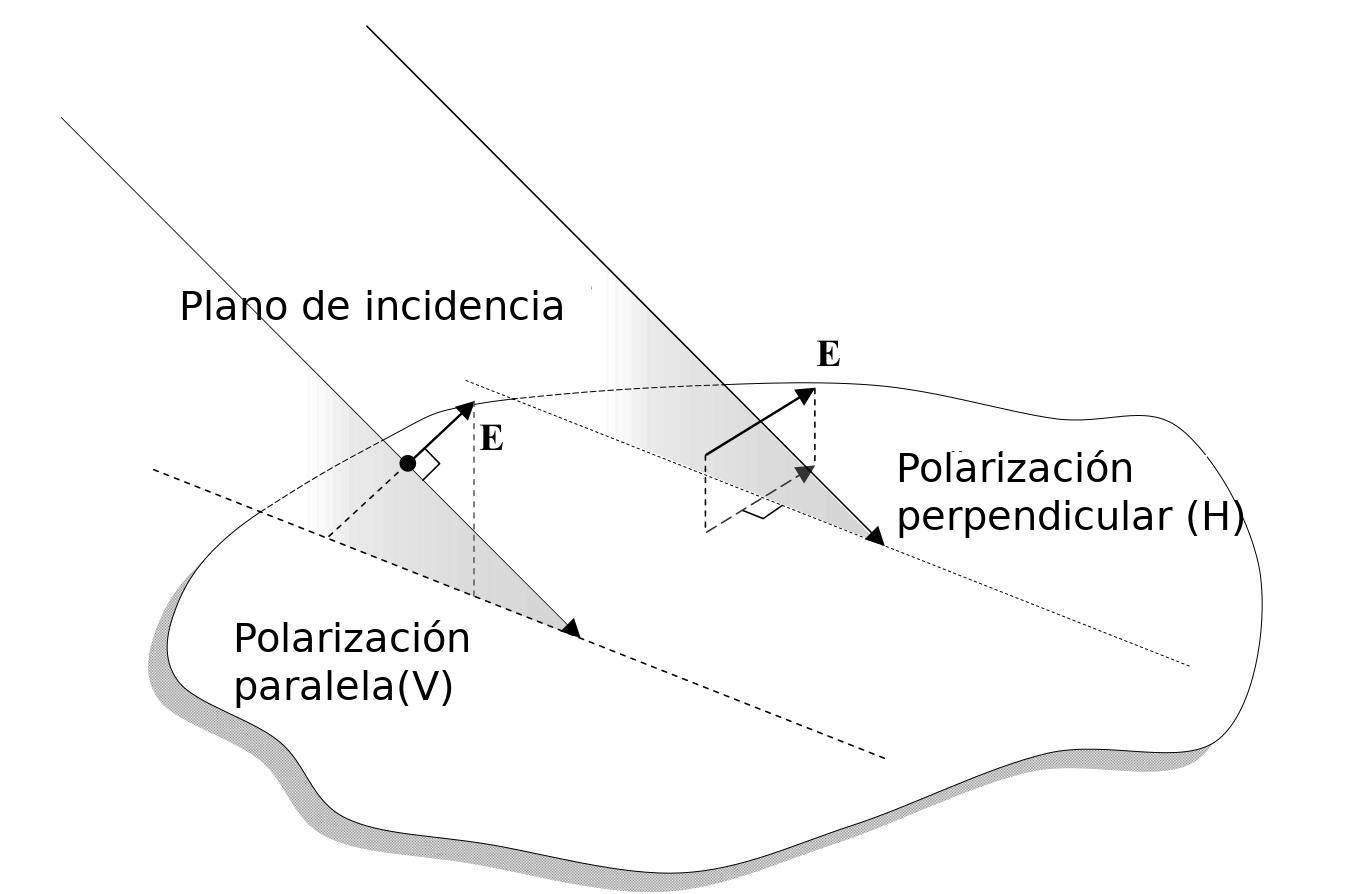
\includegraphics[width=0.6\textwidth]{fig:polarizacion.png}
    \caption{Detección de cambios en ámbitos urbanos.}
    \label{}
  \end{figure}
\end{frame}
%--- Next Frame ---%

\begin{frame}{\secname : \subsecname}
  \begin{figure}
    \centering
    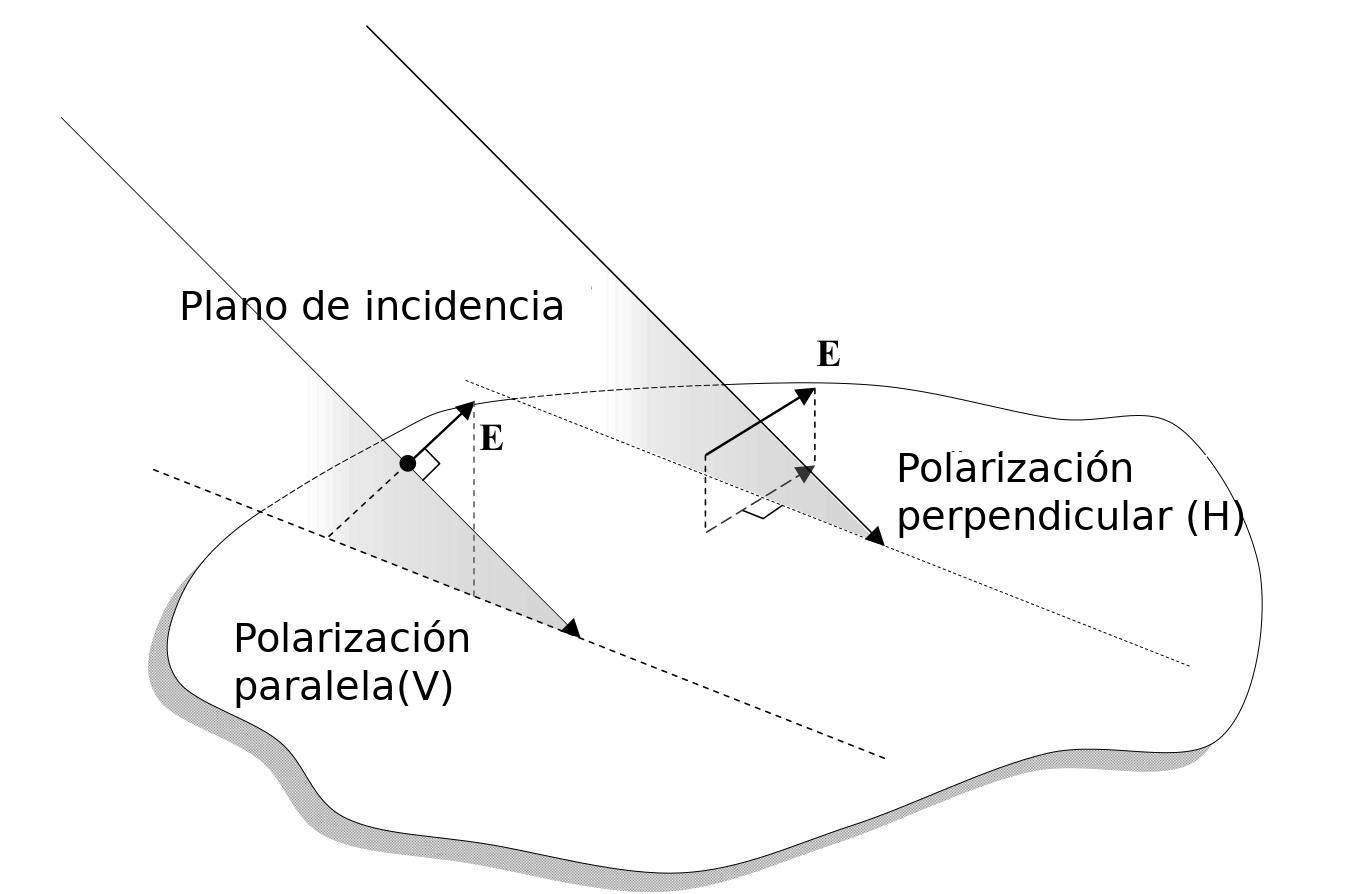
\includegraphics[width=0.6\textwidth]{fig:polarizacion.png}
    \caption{Deformación de la superficie por erupciones volcánicas.}
    \label{}
  \end{figure}
\end{frame}
%--- Next Frame ---%

\begin{frame}{\secname : \subsecname}
  \begin{figure}
    \centering
    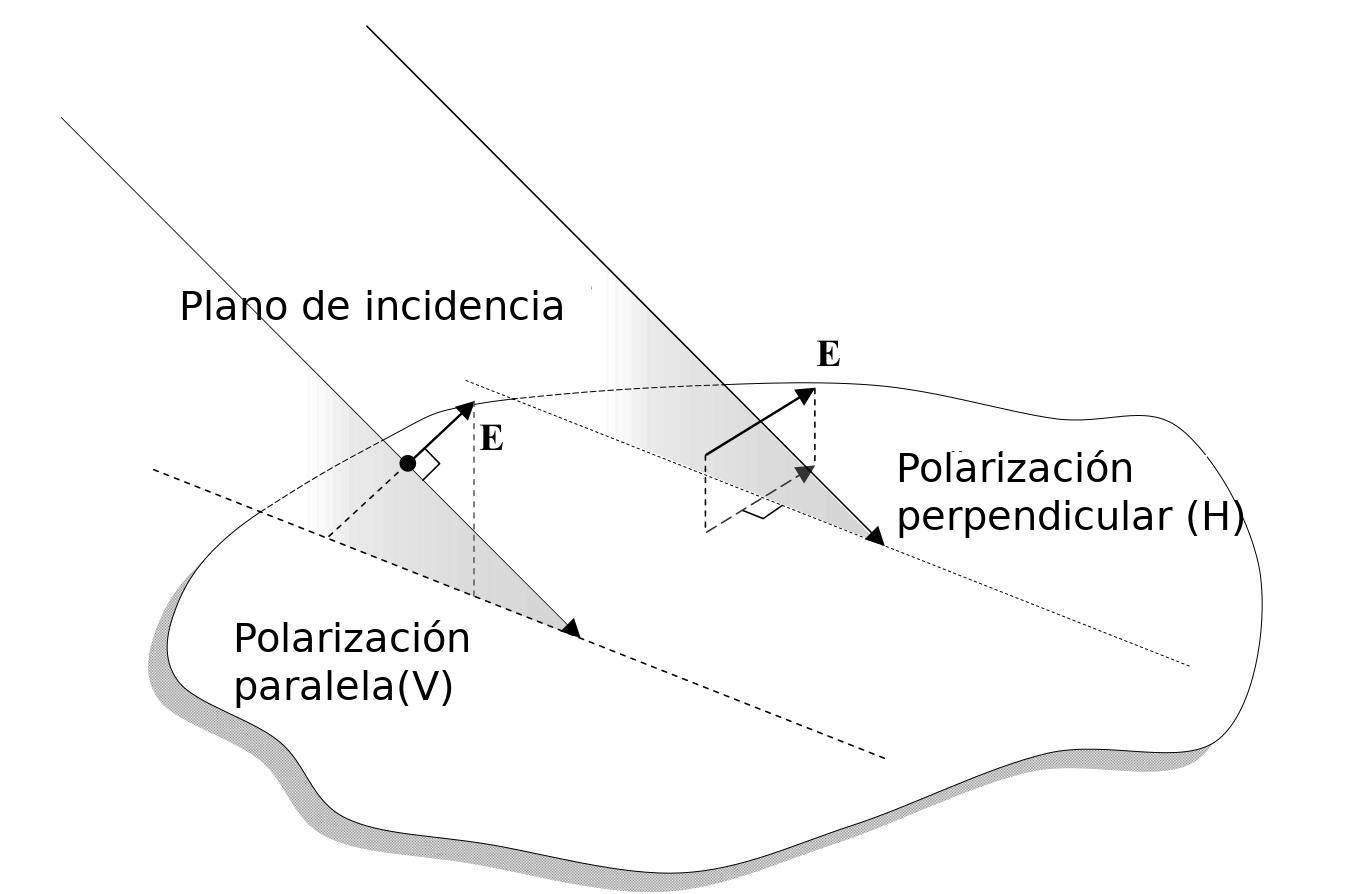
\includegraphics[width=0.6\textwidth]{fig:polarizacion.png}
    \caption{Detección de subsidencia por métodos interferométricos.}
    \label{}
  \end{figure}
\end{frame}
%--- Next Frame ---%

\begin{frame}{\secname : \subsecname}
  \begin{figure}
    \centering
    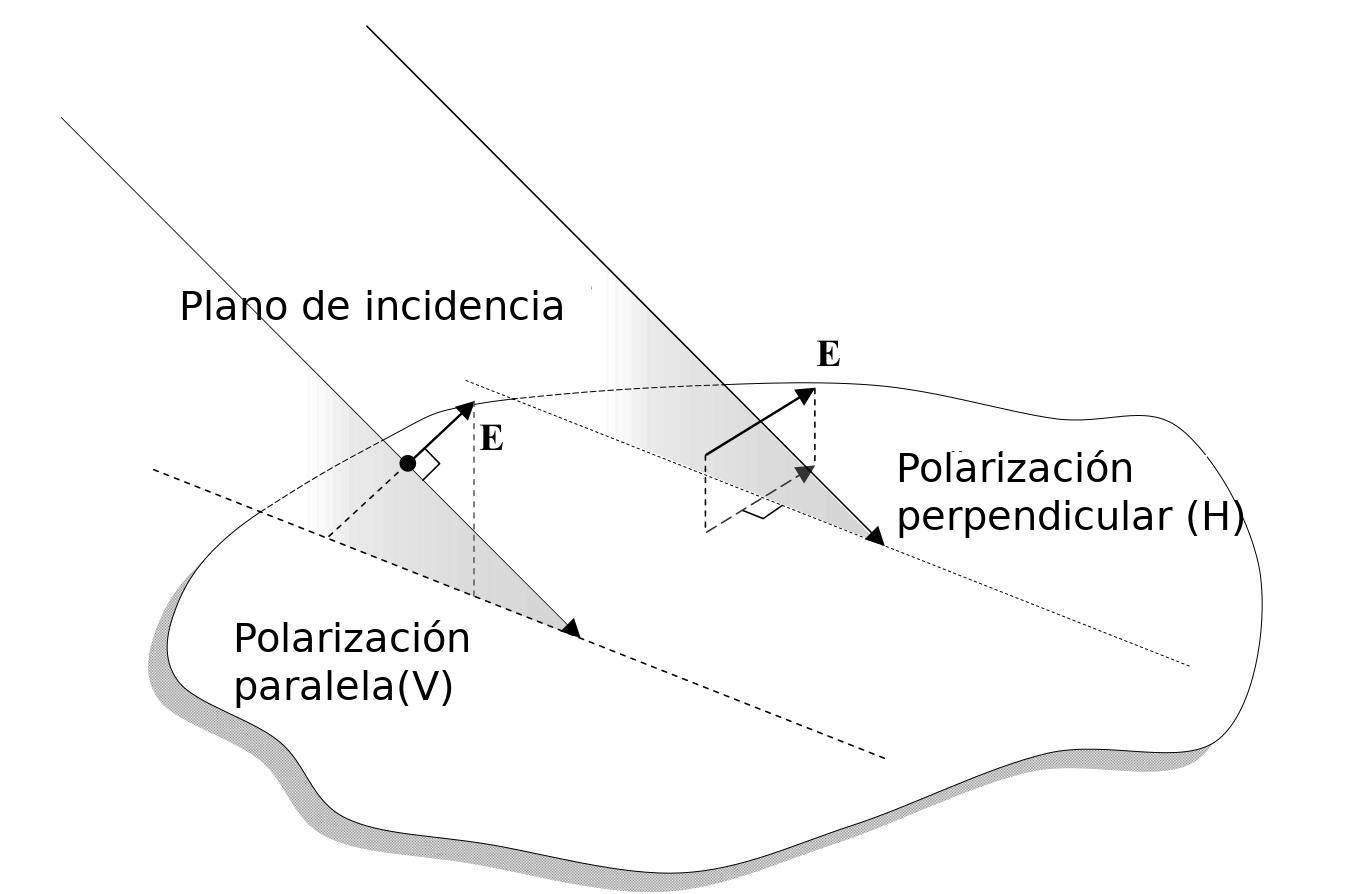
\includegraphics[width=0.6\textwidth]{fig:polarizacion.png}
    \caption{Detección de subsidencia por métodos interferométricos.}
    \label{}
  \end{figure}
\end{frame}
%--- Next Frame ---%


\begin{frame}{\secname : \subsecname}
  \begin{figure}
    \centering
    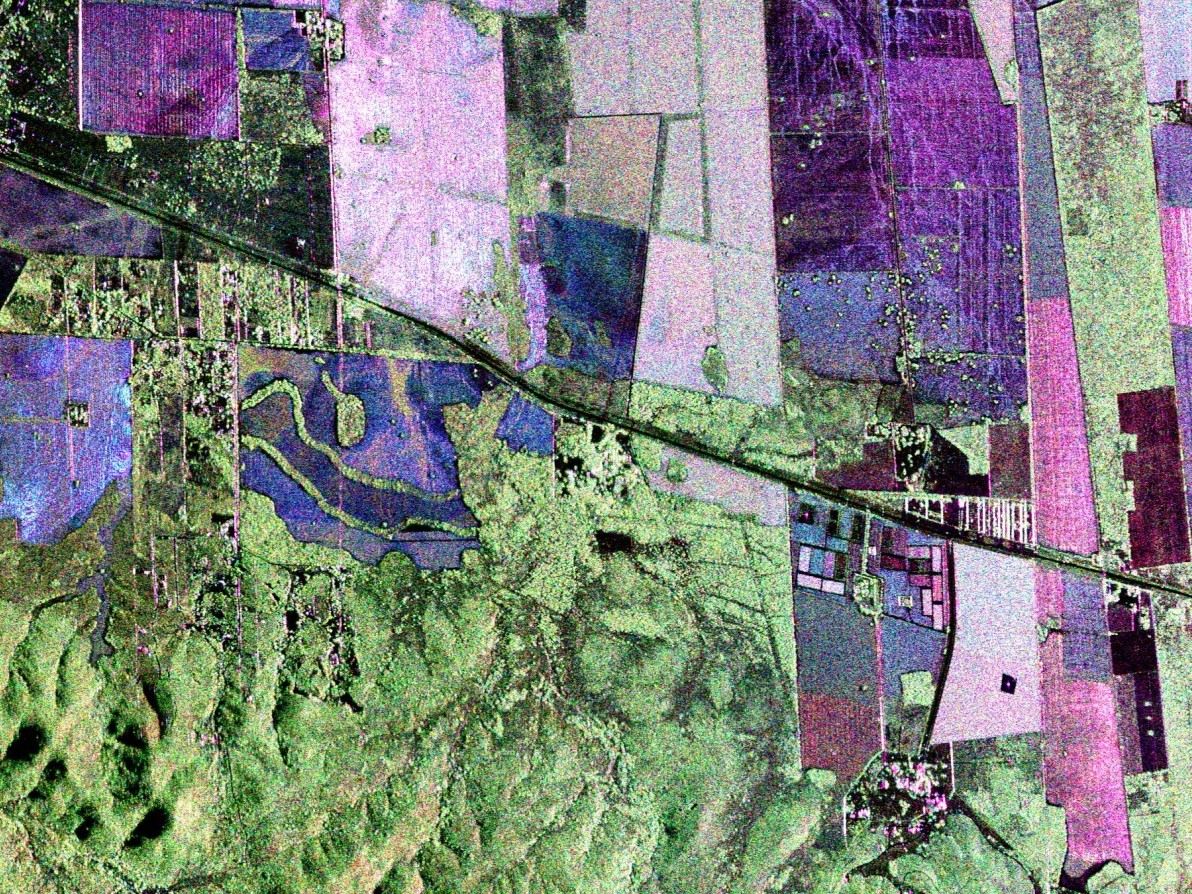
\includegraphics[width=0.5\textwidth]{fig:rgbpauli}
    \caption{Descomposición de Pauli en combinación RGB.}
    \label{}
  \end{figure}
\end{frame}
%--- Next Frame ---%

\begin{frame}{\secname : \subsecname}
Muchas gracias.
\end{frame}
%--- Next Frame ---%


\end{document}
